\documentclass[11pt,a4paper]{article}
%\setlength{\parindent}{4em} % longitud sagnat 1a línia
%\setlength{\parskip}{1em} % espai entre paràgrafs
%\usepackage[font=small,labelfont=bf]{caption} % mida font figures
\usepackage[utf8]{inputenc}
\usepackage[catalan]{babel}
\usepackage{amsmath}
\usepackage{amsfonts}
\usepackage{amssymb}
\usepackage[export]{adjustbox}
\usepackage{tabularx}
\usepackage[table]{xcolor}
\usepackage{float}
\usepackage{url}
\usepackage{hyperref}
\hypersetup{
    colorlinks=true,
    linkcolor=black,
    filecolor=black,      
    urlcolor=blue,
    citecolor=blue,
}
\usepackage{graphicx}
\usepackage{subcaption}
\usepackage{mwe}
\graphicspath{ {images/} }
\usepackage{chapterbib} 
\usepackage{listings}
\lstset{basicstyle=\ttfamily\small,literate={-}{{-\allowbreak}}{1}}
\author{Sergio González Rubio}
\title{testDEX: Un DEX simple en la xarxa Elrond}
\date{today}
%idea: https://tex.stackexchange.com/questions/249415/set-font-size-for-footnotes
\makeatletter
\renewcommand\footnotesize{%
   \@setfontsize\footnotesize\@ixpt{9}%
   \abovedisplayskip 8\p@ \@plus2\p@ \@minus4\p@
   \abovedisplayshortskip \z@ \@plus\p@
   \belowdisplayshortskip 4\p@ \@plus2\p@ \@minus2\p@
   \def\@listi{\leftmargin\leftmargini
               \topsep 4\p@ \@plus2\p@ \@minus2\p@
               \parsep 2\p@ \@plus\p@ \@minus\p@
               \itemsep \parsep}%
   \belowdisplayskip \abovedisplayskip
}
\makeatother

\begin{document}

\begin{titlepage}

\includegraphics[scale=0.2,right,valign=t]{uoc-logo.png}
\vspace*{\fill}
\begin{flushleft}
{\LARGE \textbf{testDEX: Un DEX simple en la xarxa Elrond}}
\end{flushleft}
\begin{flushleft}
\textbf{Sergio González Rubio}\\
Màster universitari de Ciberseguretat i Privadesa\\
Sistemes de blockchain
\end{flushleft}
\begin{flushleft}
\textbf{Consultor}: Josep Lluís de la Rosa Esteva\\
\textbf{Professor}: Victor Garcia Font
\end{flushleft}
\begin{flushleft}
\today
\end{flushleft}
\end{titlepage}


\begin{titlepage}
\vspace*{\fill}
\begin{flushleft}

\includegraphics[scale=1,left]{licencia-cc.png}
Aquesta obra està subjecta a una llicència de\\
Reconeixement-NoComercial-SenseObraDerivada\\
\href{http://creativecommons.org/licenses/by-nc-nd/3.0/es/}{3.0 Espanya de Creative Commons}
\end{flushleft}
\end{titlepage}

\begin{center}
\textbf{FITXA DEL TREBALL FINAL}
\end{center}
\begin{tabularx}{\textwidth}{|X|X|}
\hline 
\textbf{Títol del treball:} &\cellcolor{gray!25} \textit{testDEX: Un DEX simple en la xarxa Elrond} \\ 
\hline 
\textbf{Nom de l'autor:} &\cellcolor{gray!25} \textit{Sergio González Rubio} \\ 
\hline 
\textbf{Nom del consultor/a:} &\cellcolor{gray!25} \textit{Josep Lluís de la Rosa Esteva} \\ 
\hline 
\textbf{Nom del PRA:} &\cellcolor{gray!25} \textit{Victor Garcia Font} \\ 
\hline 
\textbf{Data de lliurament (mm/aaaa):} &\cellcolor{gray!25} \textit{juny/2022} \\ 
\hline 
\textbf{Titulació o programa:} &\cellcolor{gray!25} \textit{Màster universitari de Ciberseguretat i Privadesa} \\ 
\hline 
\textbf{Àrea del treball final:} &\cellcolor{gray!25} \textit{Sistemes de blockchain} \\ 
\hline 
\textbf{Idioma del treball:} &\cellcolor{gray!25} \textit{Català} \\ 
\hline 
\textbf{Paraules clau:} &\cellcolor{gray!25} \textit{Elrond, blockchain, EGLD, smart contract, swap} \\ 
\hline
\end{tabularx} 
\begin{tabularx}{\textwidth}{|X|}
\textbf{Resum del treball:}  \\ 
\hline 
\cellcolor{gray!25} L'adveniment Bitcoin i posteriorment d'Ethereum varen definir les bases de la tecnologia \textit{blockchain}. Cal destacar que han suposat una disrupció tecnològica, econòmica i fins i tot política, despertant un interès acadèmic creixent i nous casos d'ús. En aquest context, es presenten reptes per aconseguir una descentralització plena que sigui capaç de substituir els sistemes centralitzats tradicionals de transaccions electròniques i moviment de capitals. Alt consum d'energia, baixa taxa de transaccions, escalabilitat, seguretat o interoperabilitat són alguns dels reptes plantejats per les tecnologies actuals de \textit{blockchain} que resol Elrond. Aquest treball presenta un exemple d'implementació de \textit{swaps} entre criptovalors amb l'objectiu de comprovar que la proposta de \textit{blockchain} pública d'Elrond ha vençut les limitacions actuals de Bitcoin i Ethereum. \\
\hline 
\textbf{Abstract:}  \\ 
\hline 
\cellcolor{gray!25} The advent of Bitcoin and later of Ethereum described the foundations of blockchain technology. It should be noted that they have led to a technological, economical and even political disruption, arousing growing academic interest and new use cases. In this context, we are being challenged to achieve full decentralization that is capable of replacing traditional centralized systems of electronic transactions and movements of capital. High energy consumption, low transaction rates, scalability, security or interoperability are some challenges of current blockchain technologies that Elrond solves. This paper presents an example of the implementation of swaps between tokens in order to verify that Elrond's public blockchain proposal has overcome the current limitations of Bitcoin and Ethereum. \\
\hline 
\end{tabularx} 
\newpage 


\tableofcontents
\newpage


\listoffigures
\newpage


\section{Introducció}

\subsection{Context i justificació del treball}
\label{sub:context}
El \textit{white paper} de \textbf{Bitcoin} fou presentat l'any 2008 per una o diverses persones ocultes rere el pseudònim de Satoshi Nakamoto \cite{nakamoto2008}. Tot i que existien intents anteriors\footnote{Per exemple el ``\textit{b-money}'' de W. Dai (1998) \cite{dai1998}, el ``\textit{Reusable Proofs of Work}'' de H. Finney (2005) \cite{finney2005} o el ``\textit{Bit gold}'' de N. Szabo (2008) \cite{szabo2008}.}, fou la primera solució ``creïble'' \cite{vuterin2014} que va permetre transferir fons sense la intervenció de terceres parts (cosa que inclou a bancs centrals encarregats d'emetre la moneda). Gràcies a la implementació d'un programari client –lliure i de codi obert– s'estableix una xarxa d'igual a igual (\textit{peer-to-peer}) on es connecten nodes –no controlats– que verifiquen i emmagatzemen en una base de dades pública la comptabilitat dels moviments entre usuaris de la xarxa. Les operacions s'agrupen en blocs, que s'enllacen i xifren per assegurar que no hi hagi modificacions malicioses posteriors. Els càlculs per realitzar el xifratge tenen cert nivell de dificultat i comporten una despesa energètica considerable, per aquest motiu s'incentiva els nodes ``miners'' amb una recompensa quan aconsegueixen crear un nou bloc a la cadena. Per això es coneix aquesta tecnologia com a \textit{blockchain}\footnote{No és l'objectiu del present treball explicar els sistemes de \textit{blockchain}, però una gran exposició gràfica la realitza A. Brownworth \cite{brownworth1,brownworth2}.}. Així mateix, com afirma V. Buterin \cite{vuterin2014}, l'altra gran aportació és la manera com aplica el concepte de \textit{Proof-of-Work} (PoW) perquè els nodes arribin a un consens per validar les transaccions solucionant certs problemes (com, per exemple, el de la doble despesa). Amb PoW es pretén evitar que nodes de la xarxa tinguin comportaments indesitjats. Com ja s'ha remarcat, a Bitcoin els càlculs de xifratge per crear un nou bloc comporten molta feina computacional, però la validació d'un bloc ja creat requereix un esforç molt inferior. Si dos nodes distribueixen simultàniament diferents versions del següent bloc, el que tingui la cadena més llarga serà el que els nodes acceptin com a vàlid i descartaran la resta \cite{nakamoto2008}. Finalment, el protocol de Bitcoin també disposa d'un llenguatge de \textit{scripting}, encara que amb limitacions importants (per exemple, no és Turing complet i no té estat \cite{vuterin2014}). 

El 2014 V. Buterin va presentar el \textit{white paper} d'\textbf{Ethereum} \cite{vuterin2014} (la xarxa es va posar en producció el 30 de juliol de 2015 \cite{tual2015}). Igual que passa amb Bitcoin, s'utilitza el concepte PoW com a mecanisme de consens entre nodes, però s'incorpora un llenguatge anomenat ``Solidity'' (que sí que és Touring complet) per a la creació de ``\textit{smart contracts}'' i d'aplicacions descentralitzades (o ``DApps''). Els contractes intel·ligents són programes desplegats (o guardats) a la cadena de blocs que s'executen automàticament quan es compleixen certes condicions. A més, una DApp és una aplicació que funciona sense la necessitat de servidors centrals (gràcies a la tecnologia descrita). En el moment en què redacto aquestes línies, la versió d'Ethereum 2.0 ``Serenity'' encara no està completament desenvolupada. Aquest nou \textit{fork} ha d'introduir millores com substituir el PoW per \textit{Proof-of-Stake} (PoS), per reduir el consum d'energia, o com aplicar tècniques de \textit{sharding} per augmentar l'eficiència (la versió actual de la xarxa no arriba a suportar les 20 transaccions per segon \cite{mech2018}).

Amb Bitcoin i Ethereum consolidats, ``The Elrond Team'' va publicar el 19 de juny de 2019 el \textit{white paper} d'una nova solució de cadena de blocs pública sota el títol ``\textit{\textbf{Elrond}: A Highly Scalable Public Blockchain via Adaptive State Sharding and Secure Proof of Stake}''. Entre els reptes que plantejaren \cite{elrond2022, elrond2019}:
\begin{itemize}
    \item Descentralització plena.
    \item Seguretat robusta de les transaccions, prevenint qualsevol vector d'atac conegut.
    \item Alta escalabilitat, arribant al nivell de rendiment d'algun dels serveis equiparables amb arquitectura centralitzada.
    \item Eficiència a tots els serveis de xarxa amb el mínim consum energètic i esforç computacional.
    \item Millora de l'emmagatzematge i la sincronització de dades.
    \item Interoperabilitat entre cadenes de blocs des del disseny.
\end{itemize}
Tot i la data de publicació del \textit{white paper}, l'equip d'Elrond assegura que el seu \textit{mainnet} és actiu des de l'any 2018. A més, citen com a aconseguides en la data de redacció del present treball les següents fites \cite{elrond2022, mincul2021}:
\begin{itemize}
    \item Primera arquitectura de \textit{blockchain} en producció amb fragmentació d'estat (\textit{state sharding}).
    \item 1,5k TPS (escalable a més de 100k TPS\footnote{S'han fet proves a la \textit{testnet} amb pics de més de 260k TPS \cite{elrond2022}.}), latència de 6s i cost de \$0,001 per transacció.
    \item Maiar App\footnote{\url{https://maiar.com/}} (moneder mòbil d'Elrond), Elrond Web Wallet\footnote{\url{https://wallet.elrond.com/}} i Maiar DeFi Wallet\footnote{Per aconseguir el \textit{plugin} per al teu navegador: \url{https://getmaiar.com/defi}}.
    \item \textit{Smart Contracts}, \textit{Staking \& Delegation}, \textit{Tokens}.
    \item Maiar DEX\footnote{\url{https://maiar.exchange/}}.
    \item DeFi 2.0: Préstecs, sintètics.
    \item Validat mitjançant múltiples auditories per part de l'empresa Trail of Bits\footnote{\url{https://www.trailofbits.com/}} i d'altres.
\end{itemize}
Referent al darrer punt, he cercat informació sobre quines auditories s'han fet i la informació que he trobat és escassa (pareix que per qüestions de seguretat han estat majoritàriament auditories internes \cite{mincub2019}). Sí que apareix un acord de col·laboració per emprar les eines de l'empresa Runtime Verification\footnote{\url{https://runtimeverification.com/}} i que s'han oferit recompenses a \textit{white-hat hackers} \cite{bounties01, mincub2021}.

Tot i que hi ha altres projectes prometedors com Solana, Avalanche, Tron o Tezos \cite{baro2021}, en la meva opinió, l'evolució d'Elrond des de l'aparició del seu \textit{white paper} dona peu a parar el nostre interès acadèmic en aquest projecte i no en els altres. És per aquest motiu que es proposa desenvolupar un \textbf{DEX} molt simple que permeti fer intercanvis entre diferents criptomonedes emprant el protocol \textbf{\textit{automated market makers}} (AMM) \cite{cryptopedia2021} amb la intenció de \textbf{posar a prova la xarxa d'Elrond}.

\subsection{Objetius del treball}\label{sub:objectius}
A nivell molt genèric, els quatre grans objectius que pretenc assolir són:
\begin{itemize}
    \item L'anàlisi i estudi de la tecnologia de \textit{blockchain} d'Elrond des d'un punt de vista acadèmic.
    \item La definició d'una proposta d'arquitectura per desenvolupar DApps en la xarxa d'Elrond.
    \item El desenvolupament d'un exemple pràctic usant l'arquitectura anterior.
    \item La definició de proves per comprovar característiques de la xarxa d'Elrond.
\end{itemize}

Vull destacar en aquest apartat que no he trobat cap altre treball acadèmic sobre la xarxa d'Elrond en llengua catalana. S'ha de destacar que el contingut de la secció \ref{sec:revelrond} és una tasca de selecció, síntesi i traducció de les fonts citades en les respectives subseccions (bàsicament, \cite{elrond2022} i \cite{elrond2019}). Òbviament, l'autor no va participar en la creació de la xarxa d'Elrond i, per tant, l'autoria del conceptes que s'exposen és de The Elrond Team. 

\subsection{Enfocament i mètode seguit}
Després de revisar ràpidament l'estat de l'art de les tecnologies \textit{blockchain}, ha estat una aposta personal fer servir Elrond. És un projecte novedós i sé que, per aquest motiu, disposaré de menys bibliografia que amb Bitcoin o Ethereum. Aquest darrer fet espero que, més que ser una cosa negativa, em permeti fins i tot trobar nous objectius a mesura que vagi investigant. Així mateix, una bona planificació del projecte és ben necessària, on vull destacar que la fase d'investigació es realitzarà de forma paral·lela a la resta.

Les \textbf{fases} que es desenvoluparan són les següents:
\begin{itemize}
    \item \textbf{Plantejament del problema}: Es duu a terme una entrevista amb Josep Lluís de la Rosa Esteva i es pacta desenvolupar un \textbf{DEX} emprant el protocol AMM amb el propòsit de provar i comprovar algunes de les característiques de la tecnologia d'Elrond. Com s'ha comentat, previ a l'entrevista, va haver-hi una feina d'investigació ràpida sobre l'estat de l'art en els sistemes \textit{blockchain}.
    \item \textbf{Pla de treball}: Es definiran els recursos necessaris per fer el projecte, les tasques a fer i la seva temporalització.
    \item \textbf{Revisió de la tecnologia d'Elrond}: Es descriurà a tall de resum la tecnologia i s'enumeraran els recursos que hi ha disponibles per desenvolupar en aquesta xarxa.
    \item \textbf{testDEX}:
    \begin{itemize}
    	\item \textbf{Anàlisi}: Definició dels requisits i dels models relacionats amb aquests. 
    	\item \textbf{Disseny}: Realització dels models que defineixen el disseny del sistema i l'arquitectura.
    	\item \textbf{Implementació}: Escriptura del codi font.
    	\item \textbf{Posada en producció}: Desplegament en producció del projecte.
    	\item \textbf{Proves}: La fase de proves es durà a terme de forma paral·lela a la implementació i a la de posada en producció. S'han de definir uns criteris de qualitat mínims abans de posar l'aplicatiu en producció (on es continuarà realitzant proves).
    \end{itemize}
    \item \textbf{Redacció de la memòria}: Es farà de forma paral·lela mentre es duen a terme les fases anteriors.
    \item \textbf{Creació del vídeo de la presentació final}: Necessari per defensar el treball.
    \item \textbf{Investigació i formació}: Pel plantejament inicial del treball, es durà a terme a la vegada que es realitzen la resta de fases.
\end{itemize}

\subsection{Planificació del treball}
Els recursos necessaris per desenvolupar el projecte són mínims: Un ordinador personal amb el seu sistema operatiu i un editor de codi (\textit{Visual Studio Code}\footnote{Existeix el \textit{plugin} ``Elrond IDE'': \url{https://marketplace.visualstudio.com/items?itemName=Elrond.vscode-elrond-ide}}). Per altra banda, les tasques a realitzar han estat enumerades en el punt anterior i seran descrites en el seu apartat corresponent. Gràficament en un diagrama de Gantt queden de la següent forma:

\begin{figure}[h]
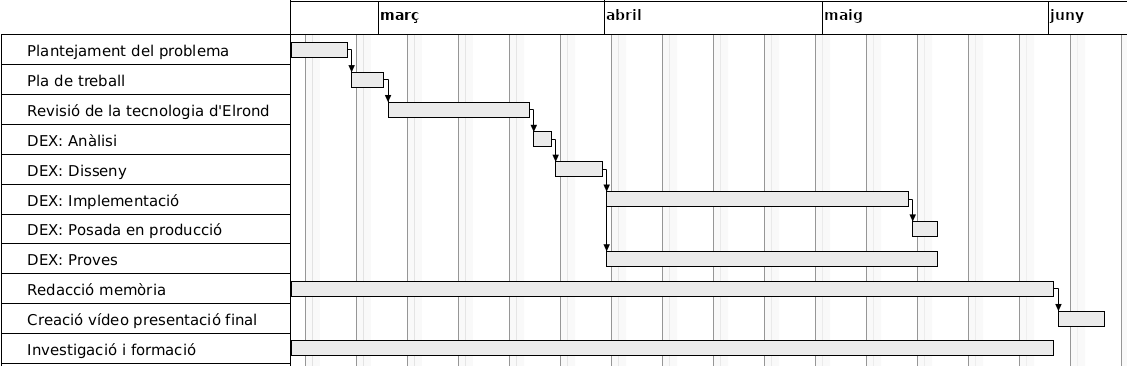
\includegraphics[width=1\textwidth]{gantt.png}
\centering
\caption{Diagrama de Gantt del projecte (creat amb GNOME Planner 0.14.6).}
\end{figure}

La següent figura presenta la temporalització de les fases del projecte, s'ha de considerar que un dia de feina correspon a una jornada de quatre hores:
\begin{figure}[h]
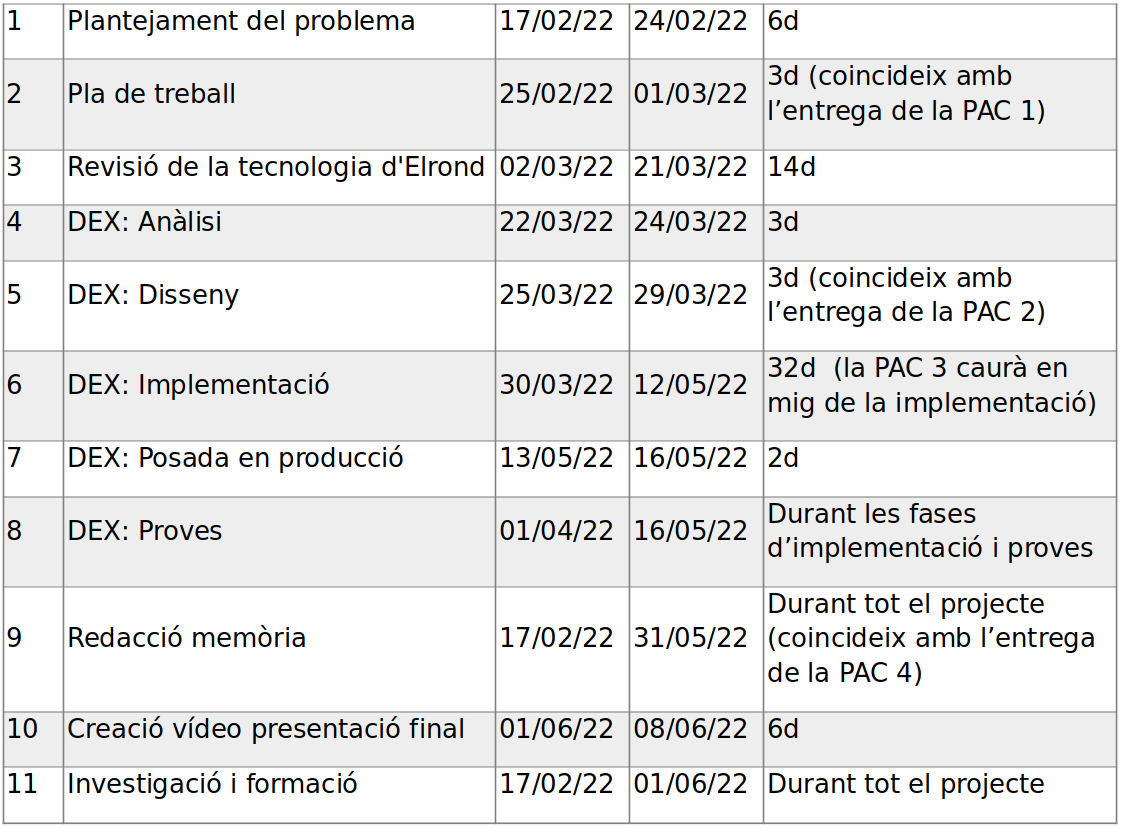
\includegraphics[width=0.85\textwidth]{gantttemp.png}
\centering
\caption{Temporalització del projecte.}
\end{figure} 

\subsection{Breu sumari de productes obtinguts}
El present treball bàsicament aporta:
\begin{itemize}
\item Un \textbf{revisió teòrica de la tecnologia} d'Elrond.
\item Un \textbf{exemple pràctic d'arquitectura} per a aplicacions descentralitzades emprant aquesta tecnologia amb testDEX.
\item Un \textbf{\textit{script} en Python per testejar el rendiment} de la xarxa.
\end{itemize}

\subsection{Breu descripció dels altres capítols de la memòria}
En la secció \ref{sec:revelrond} ``Revisió de la tecnologia d'Elrond'' es descriuen els conceptes generals d'Elrond, el funcionament bàsic de la seva tecnologia i els productes de l'empresa disponibles. La \ref{sec:testdex} ``testDEX'' presenta les fases del desenvolupament de l'aplicació de mostra que aplica els conceptes teòrics exposats. En la secció \ref{sec:con} ``Conclusions'' es revisa de forma crítica el resultat del present treball. La \ref{sec:glo} és un compendi d'acrònims i termes destacables d'aquesta memòria. El \ref{sec:bib} enumera la bibliografia emprada. Finalment, en el \ref{sec:ann} ``Annexos'' apareix un petit manual d'usuari de la DApp ``testDEX''.

\clearpage

\section{Revisió de la tecnologia d'Elrond}\label{sec:revelrond}

\subsection{Visió general de l'arquitectura}
Elrond és una cadena de blocs\footnote{En el present treball empraré indistintament ``\textit{blockchain}'' i ``cadena de blocs'' (traducció del terme proposada pel Termcat).} pública i d'alt rendiment. Altres punts a destacar són \cite{elrond2022, elrond2022-2}:
\begin{enumerate}
  \item \textbf{Entitats (usuaris i nodes)}: Els usuaris despleguen transaccions a la xarxa, en forma de transferència de valor o executant un \textit{smart contract}. Per altra banda, els nodes són dispositius en la xarxa que executen el programari d'Elrond i processen les transaccions.
  \item \textbf{\textit{Validadors}}: Nodes de la xarxa Elrond amb almenys 2500 EGLD en \textit{staking} (o bloquejats\footnote{El Termcat encara no ha traduït el terme, és una traducció pròpia que penso que fa entendre el concepte.}) que processen les transaccions i asseguren la xarxa per la seva participació en el mecanisme de consens per validar els blocs (seran recompensats amb les tarifes –\textit{fees}– de les transaccions).
  \item \textbf{\textit{Shards\footnote{No hi ha entrada al Termcat pel terme ``shard'', jo l'he traduït per ``fragment'' (empraré ambdues paraules indistintament en el present treball).}}}: Particions de la xarxa d'Elrond que permeten escalar-la. La feina de cada \textit{shard} és gestionar una part de l'estat i processar paral·lelament la corresponent part de la transacció.
  \item \textbf{\textit{Adaptive State Sharding}}: Divisió i unió dinàmica de \textit{shards} segons el nombre de validadors disponible i càrrega de la xarxa. S'aplica a tots els nivells (transacció, dades i xarxa) de forma adaptativa.
  \item \textbf{\textit{Secure Proof of Stake}}: Els blocs són validats per consens entre els validadors del grup de consens (valgui la redundància), que és completat en dues passes de comunicació emprant una modificació de les signatures múltiples de Boneh-Lynn-Shacham (BLS) \cite{Boneh2004}. El grup de consens és seleccionat aleatòriament i només és possible conèixer la seva composició amb una ronda d'antelació.
  \item \textbf{Alta resiliència}: Capacitat de recuperar-se d'atacs maliciosos pel canvi de nodes entre els \textit{shards} (en cada ``època'' un terç dels nodes seran reubicats per prevenir connivències entre els mateixos).
  \item \textbf{Font d'aleatorietat segura}: Utilitzant la signatura BLS, cosa que la fa no esbiaixada i impredictible.
  \item \textbf{Elrond WASM VM}: Màquina virtual específica que permet executar contractes intel·ligents escrits en qualsevol llenguatge de programació que es permeti compilar amb  \textit{WebAssembly}\footnote{\url{https://webassembly.org/}}.
  \item \textbf{Contractes intel·ligents}: Que s'executaran emprant l'\textit{Adaptative State Sharding}. Elrond recomana que siguin escrits en Rust però, com s'ha dit en el punt anterior, es poden utilitzar altres llenguatges. Una característica única, comparant per exemple amb Ethereum, és que es poden modificar els \textit{smart contracts} després de ser desplegats \cite{cwirko01} (per exemple per corregir errors).
  \item \textbf{Execució ràpida de transaccions \textit{cross-shard}}: Gestionada de forma nadiua a nivell de protocol fent servir un algorisme d'expedició (\textit{dispatching}) i un algorisme d'encaminament.
   \item \textbf{\textit{Metachain}}: Cadena de blocs que s'executa en un \textit{shard} especial. El seu rol principal no és processar transaccions sinó que  és notificar i autenticar les capçaleres dels blocs processats.
   \item \textbf{Elrond Gold (EGLD)}: Criptovalor (\textit{token}) nadiu de la xarxa Elrond que serveix de mitjà de pagament per a les transaccions. Ajuda en el desplegament de DApps, en l'execució de contractes intel·ligents i també s'empra com a mecanisme de pagament de recompenses per als validadors. 
\end{enumerate}

\subsection{Entitats}
\label{sub:entitat}
Bàsicament, en la xarxa Elrond hi ha dos tipus d'entitats: usuaris i nodes \cite{elrond2022}. Un \textbf{usuari} és qualsevol ens que gestioni un dels \textbf{comptes} –o més– de la xarxa Elrond. Un parell de \textbf{claus criptogràfiques} (una pública i una privada) li permetran enviar \textbf{transaccions signades} fent servir la xarxa. Els comptes tenen associat una quantitat d'EGLD que es coneix com a \textbf{balanç} i a més tenen un espai d'emmagatzematge per a valors arbitraris (com per exemple informació sobre \textbf{\textit{tokens} creats pels usuaris}). Els comptes s'identifiquen de forma unívoca per una \textbf{adreça} que coincideix amb la clau pública de l'usuari (32 bytes fent servir la representació Bech32). Normalment, els usuaris gestionen els seus parells de claus emprant unes aplicacions informàtiques que s'anomenen \textbf{carteres} (o \textit{wallets})\footnote{En el present treball empraré els termes ``cartera'' o ``moneder'' indistintament per referir-me al concepte de ``\textit{wallet}''.}.

Per altra banda, els \textbf{nodes} són dispositius connectats a la xarxa d'Elrond que realitzen les operacions sol·licitades pels seus usuaris. Els nodes poden ser passius (\textit{observers}) o actius (\textit{validators} i \textit{fishermen}). Els validadors s'encarreguen del consens, d'afegir blocs i mantenir l'estat, essent premiats per la seva contribució. Els \textbf{validadors} són identificats de forma única per una clau pública BLS de 96 bytes. Per garantir el correcte funcionament dels nodes, els validadors han de tenir en \textit{staking} com a mínim 2500 EGLD. Sense bloquejar aquesta quantitat d'EGLD, els nodes poden fer d'\textbf{observadors} (però no rebran cap recompensa). Aquests darrers són membres passius de la xarxa que poden actuar com a interfície de lectura i retransmissió. Poden ser complets (\textit{full)}, mantenint tota la història de la cadena de blocs, o lleugers (\textit{light}), mantenint només 2 èpoques de l'historial de la cadena de blocs. Finalment, trobem els \textbf{pescadors} (\textit{fishermen}). La seva tasca és verificar la validesa dels blocs després d'haver estat proposats, detectant així actors maliciosos \cite{elrond2022-2}. Rebran també una recompensa i aquest rol pot ser exercit per observadors o validadors que no formin part de la ronda de consens en curs.\footnote{No es diu explícitament en la bibliografia però investigant pels grups de Telegram d'Elrond (concretament en \url{https://t.me/ElrondValidators}) vaig descobrir que el concepte de ``\textit{fisherman}'' encara no està implementat.}

\subsection{Cronologia}
En la xarxa d'Elrond el temps s'organitza en \textbf{èpoques} (\textit{epochs}) que es subdivideixen en \textbf{rondes} (\textit{rounds}) \cite{elrond2022}. La primera ronda de la primera època (\textit{genesis round}) és especial i serveix per inicialitzar la xarxa.

Una \textbf{època} és una seqüència de rondes consecutives en què la configuració de la xarxa no canvia. El nombre de rondes en una època es calcula perquè aquesta darrera duri 24 hores (això està definit en la configuració actual i és modificable). Quan hi ha un canvi d'època s'aprofita per adaptar la topologia de la xarxa segons el nombre de validadors disponibles i càrrega de treball. En aquest precís moment també s'aprofita per acomplir amb altres tasques per tancar l'època anterior (com calcular les recompenses per als validadors).

Com es pot intuir, les \textbf{rondes} tindran una durada fixa que (actualment és configurada en 5 segons). Per l'arquitectura en \textit{shards} de la xarxa, en cada ronda només es podrà afegir un bloc a la cadena de blocs del \textit{shard}. Òbviament, si no s'arriba a consens o quan el líder del grup de consens designat és fora de línia i no pot proposar un bloc, pot haver-hi rondes en què no s'afegeixi cap bloc a la \textit{blockchain}.

S'ha de remarcar que els sistemes que implementen PoS solen dividir el temps de forma similar \cite{elrond2019}.

\subsection{\textit{Secure Proof of Stake}}
El funcionament \textit{Secure Proof of Stake} (SPoS) d'Elrond es pot desgranar en les següents passes \cite{elrond2022,elrond2019}: 
\begin{enumerate}
    \item La font d'aleatorietat per seleccionar els validadors per al consens es calcula a partir del bloc anterior, que és signat pel líder de consens –també conegut com a proposador de blocs o \textit{block proposer}– de la ronda que acaba. Això implica que aquesta font d'aleatorietat no podrà ser coneguda amb més d'una ronda d'antelació.
    \item Se selecciona el grup de consens, compost per validadors i un únic \textit{block proposer}. Una vegada coneguda la font d'aleatorietat, el procediment de tria del grup és determinista (triga menys de 100 ms\footnote{El SPoS d'Elrond es basa en la premissa que un actor malèvol només té el temps que dura una ronda per adaptar-se i intentar influir en el bloc que es proposarà.}). S'ha de considerar que per triar els nodes es té en compte la quantitat d'EGLD en \textit{staking} i una qualificació individual –revisada al final de cada època– que es basa en el comportament passat. Per exemple, es davallarà la seva puntuació si no proposa el bloc perquè és fora de línia, es detecta una activitat maliciosa, etc. Aquesta ``meritocràcia'' anima els propietaris dels nodes a tenir-los en bon funcionament. 
    \item  El líder de consens (o validació) produeix el  bloc per a la nova ronda. Si, pel motiu que sigui, no s'ha creat un bloc en una finestra de temps s'utilitzarà la font d'aleatorietat de l'últim bloc per seleccionar un nou grup de consens.
    \item El líder de consens\footnote{Per aclarir del tot aquest punt, en la bibliografia emprada, líder de consens, líder de validació i proposador de bloc (\textit{block proposer}) fan referència al mateix concepte.} envia el bloc que acaba de proposar als validadors.
    \item  Aquests darrers components del grup validen i també signen el bloc rebut, basant-se en una modificació de \textit{Practical Byzantine Fault Tolerance} (pBFT).
    \item Els validadors trameten les signatures al \textit{block proposer}.
    \item El proposador agrega les signatures i distribueix el bloc.
    \item El \textit{hash} del bloc, la signatura, les proves d'inclusió i el nombre de \textit{shard} són enviats a la \textit{Metachain}. 
\end{enumerate}

Aquestes passes es poden veure resumides en la Fig. \ref{fig:SPoS}.

\begin{figure}[h]
  \centering
  \begin{minipage}[b]{0.65\textwidth}
    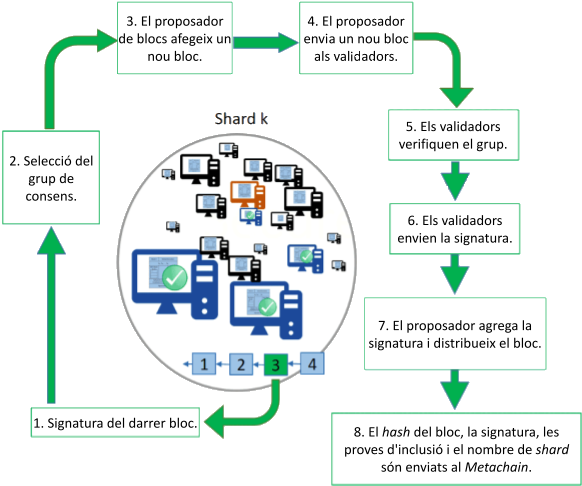
\includegraphics[width=\textwidth]{SPoS01.png}
    \caption{\textit{Secure Proof of Stake}. (Font: Modificació d'imatge dins l'apartat corresponent a SPoS a \cite{elrond2022}).}
    \label{fig:SPoS}
  \end{minipage}
  \hfill
  \begin{minipage}[b]{0.33\textwidth}
    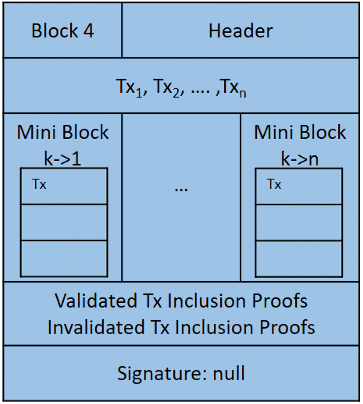
\includegraphics[width=\textwidth]{SPoS02.png}
    \caption{Estructura d'un bloc en la xarxa Elrond. (Font: Imatge dins l'apartat corresponent a SPoS a \cite{elrond2022}).}
  \end{minipage}
\end{figure}

\subsection{\textit{Adaptive State Sharding}}
El \textit{sharding} va sorgir originàriament en el camp de les bases de dades com un mètode per distribuir les dades entre múltiples màquines amb l'objectiu de suportar alt rendiment amb grans volums d'informació \cite{mongodb2021}. Elrond empra aquesta tècnica d'escalat horitzontal per particionar tant la xarxa com l'estat i processament de les transaccions amb la finalitat que diferents nodes desenvolupin la seva tasca en paral·lel (amb el consegüent augment de l'eficiència). S'ha de destacar també que s'empren els tres tipus principals de \textit{sharding} \cite{elrond2022}:

\begin{itemize}
	\item \textbf{\textit{Network sharding}}\footnote{Aquest concepte es podria traduir al català com ``fragmentació de la xarxa'' però he preferit deixar el terme anglès. El mateix passa amb \textit{transaction sharding} i \textit{state sharding}, que es podrien traduir respectivament per ``fragmentació de les transaccions'' i ``fragmentació de l'estat''.}: Gestiona com els nodes es distribueixen i agrupen entre els diferents \textit{shards}. S'ha de tenir en compte que les comunicacions dins del \textit{shard} són més ràpides que fer una propagació (\textit{broadcast}) dels missatges a tota la xarxa. Un punt molt important a destacar és que si un atacant arriba a controlar un \textit{shard} enter suposaria un greu problema de seguretat. 
	\item \textbf{\textit{Transaction sharding}}: S'ocupa la forma en què les transaccions s'assignen als \textit{shards} encarregats del seu processament. Les transaccions són assignades a un \textit{shard} de forma determinista emprant les adreces de les transaccions.
	\item \textbf{\textit{State sharding}}: Cada \textit{shard} només manté una part de l'estat. Els dos mètodes anteriors, si no es combinessin amb aquest, haurien d'emmagatzemar una còpia entera de tot l'estat. Així, si els comptes implicats en una transacció resideixen en \textit{shards} diferents, l'execució de la transacció implicaria l'intercanvi de missatges entre nodes per modificar els respectius estats. Com ja s'ha dit, per augmentar la tolerància a atacs maliciosos, quan acaba una època es redistribueixen entre els diferents \textit{shards} un subconjunt dels nodes.
\end{itemize}

Com a resultat d'aquesta fusió s'aconsegueix \cite{elrond2022}:
\begin{itemize}
	\item \textbf{Escalabilitat sense afectar a la disponibilitat}: En la Fig. \ref{fig:sharding01a} podem observar la xarxa amb només un \textit{shard}. Les figures \ref{fig:sharding01b} i \ref{fig:sharding01c} mostren una arquitectura amb dos i tres \textit{shards}\footnote{En \cite{elrond2019} es pot trobar una funció en pseudocodi amb la que calcular el nombre òptim de \textit{shards}.}. Sense entrar en detall, es pot veure que augmentant o disminuint el nombre de \textit{shards} –gràcies a la forma en què s'assignen les adreces al seu fragment– s'evita temps d'inactivitat per qüestions de configuració.
	\item \textbf{Expedició (\textit{dispatching}) ràpida i traçabilitat}: La Fig. \ref{fig:sharding01c} mostra com es calcula el \textit{shard} de destí de forma determinista (les adreces de color blau aniran al 0, les verdes a l'1 i les grogues al 2).
	\item \textbf{Eficiènia i adaptabilitat}: El sistema permet processar transaccions en paral·lel i adaptar-se a la càrrega de treball i/o estat de la xarxa. Però s'ha de destacar que la distribució dels \textit{shards} hauria de ser tan equilibrada com fos possible. Si ens fixem en la Fig. \ref{fig:sharding01c} veiem que no és equilibrada (ja que el nombre de \textit{shards} no és una potència de 2).
\end{itemize}

\begin{figure}[h]
        \centering
        \begin{subfigure}[b]{0.4\textwidth}
            \centering
            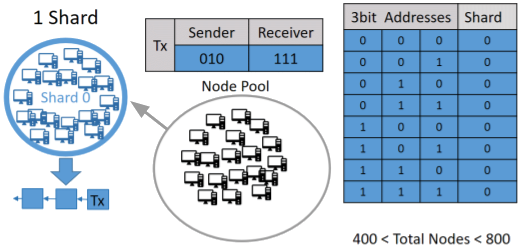
\includegraphics[width=\textwidth]{sharding01.png}
            \caption[1 \textit{shard}]%
            {{\small 1 \textit{shard}}}   
            \label{fig:sharding01a}
        \end{subfigure}
        \hfill
        \begin{subfigure}[b]{0.4\textwidth}  
            \centering 
            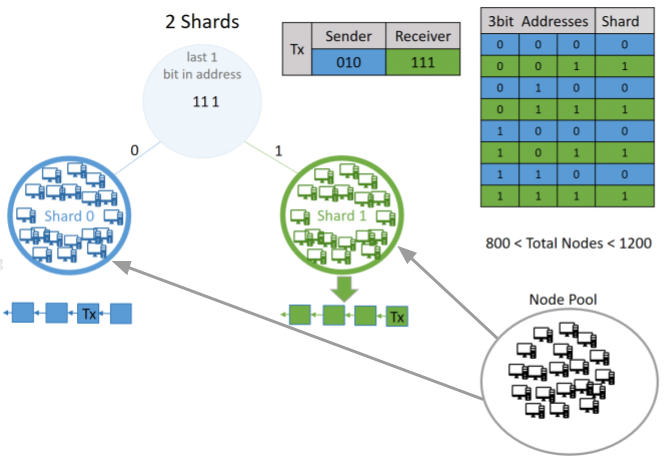
\includegraphics[width=\textwidth]{sharding02.png}
            \caption[2 \textit{shards}]%
            {{\small 2 \textit{shards}}}    
            \label{fig:sharding01b}
        \end{subfigure}
        \vskip\baselineskip
        \begin{subfigure}[b]{0.55\textwidth}   
            \centering 
            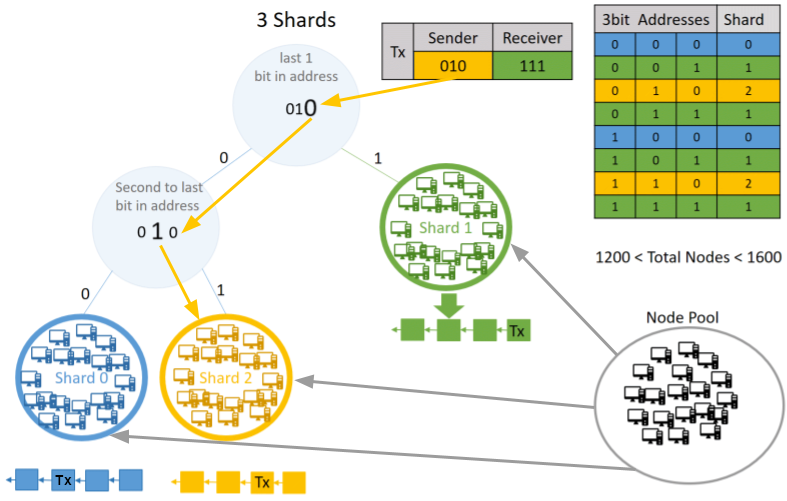
\includegraphics[width=\textwidth]{sharding03.png}
            \caption[3 \textit{shards}]%
            {{\small 3 \textit{shards}}}    
            \label{fig:sharding01c}
        \end{subfigure}
        \hfill
        \caption[La xarxa d'Elrond configurada amb un (a), dos (b) i tres (c) \textit{shards}.]
        {\small La xarxa d'Elrond configurada amb un (a), dos (b) i tres (c) \textit{shards}. (Font: Modificació d'imatge dins l'apartat \textit{Adaptive State Sharding} a \cite{elrond2022}).} 
        \label{fig:shardingtodo}
\end{figure}

Una altra cosa a destacar és que els nodes guarden una \textbf{còpia de l'estat dels seus germans (redundància)} per aportar \textbf{tolerància a fallades} (Fig. \ref{fig:shardred}).

Finalment, s'ha de remarcar el fet que els \textbf{nodes es barregin entre \textit{shards} al final de cada època} per evitar la connivència entre nodes maliciosos. Això no es fa amb tots els nodes sinó que només es redistribuirà –de forma determinista i uniforme– un nombre controlat de validadors (aquesta tasca la realitza la \textit{metachain} emprant una font d'aleatorietat procedent del bloc anterior de la metacadena). Es fa així, i no reorganitzant tots els nodes, per maximitzar la seguretat amb la mínima introducció de latències en el sistema. Els nodes triats es col·locaran als seus nous \textit{shards} en una llista d'espera durant tota l'època actual fent la resincronització amb el nou fragment. Després el node es pot convertir en un validador elegible i unir-se al \textit{shard} efectivament.\footnote{Aquest paràgraf és un resum molt breu. Per referències més detallades consultar \cite{elrond2019}.}

\begin{figure}[h]
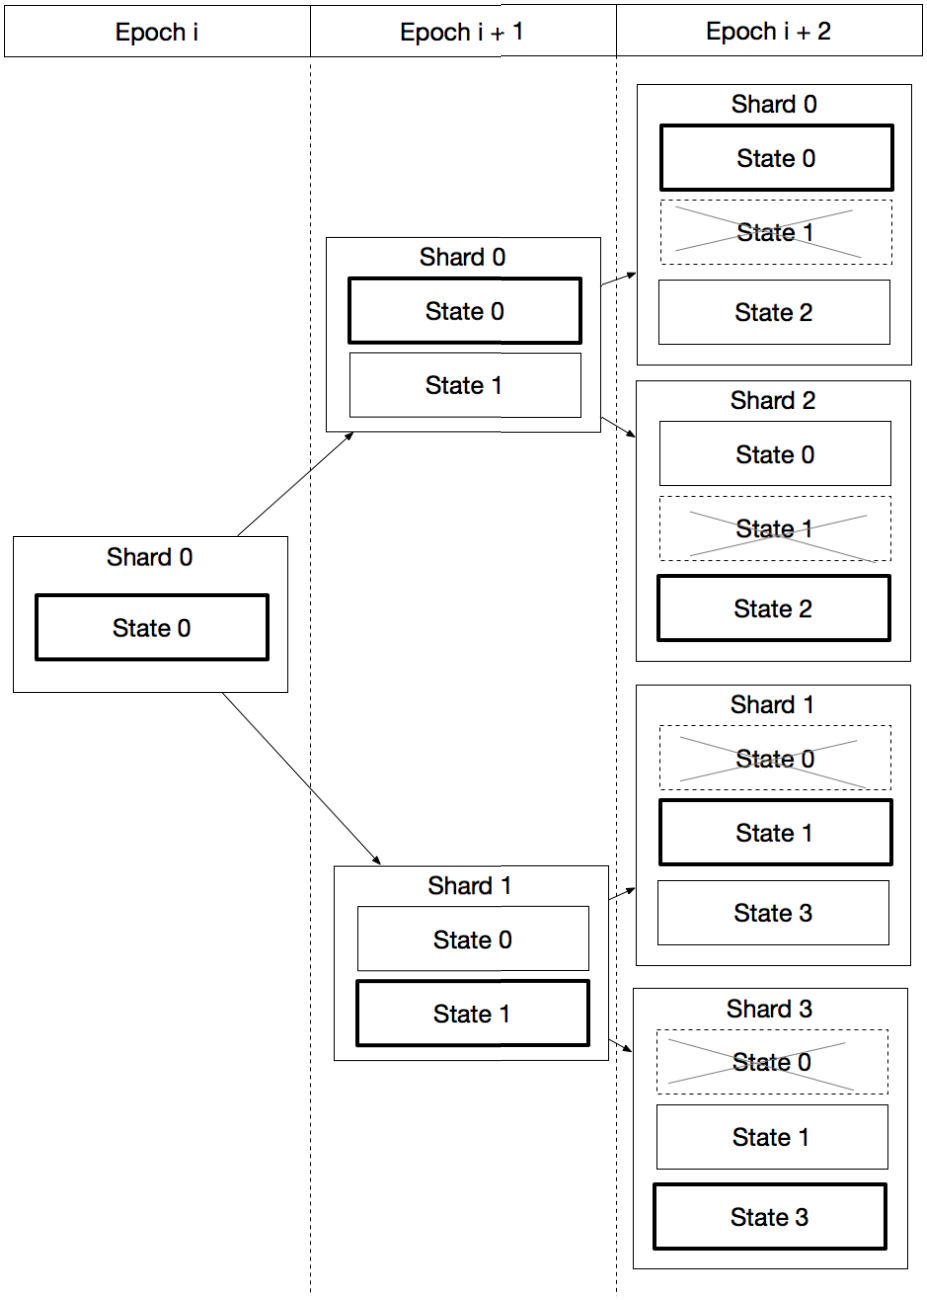
\includegraphics[width=0.4\textwidth]{shardred.png}
\centering
\caption{Redundància als \textit{shards} entre èpoques. (Font: Captura de \cite{elrond2019}).}
\label{fig:shardred}
\end{figure}

\subsection{Transaccions entre \textit{shards}}\label{sec:transshards}
Com a exemple de com s'executen les transaccions entre diferents \textit{shards} i com es comuniquen amb la \textit{metachain}, emprarem una \textbf{arquitectura amb només dos \textit{shards}}. Imaginem que un usuari des del seu \textit{wallet} amb una adreça dins del \textit{shard} 0 envia EGLD a l'adreça d'altre \textit{wallet} que es troba en el \textit{shard} 1 (Fig. \ref{fig:shardingtrans}). L'estructura dels blocs estarà formada per \cite{elrond2019}:
\begin{itemize}
	\item \textbf{Capçalera} (\textit{header}): Conté la informació referent al bloc (\textit{nonce}, \textit{round}, \textit{proposer}, \textit{validators}, \textit{timestamps}, etc.).
	\item \textbf{Llista de miniblocs}: Per a cada \textit{shard} hi haurà un minibloc que contindrà transaccions a executar. 	S'ha de destacar que un minibloc és la unitat atòmica de processament, això significa que o es processen totes les transaccions del minibloc o no es processa cap (en aquest darrer cas, es posposarà l'execució al següent \textit{round}). Dins d'un mateix bloc, poden aparèixer diversos miniblocs amb el mateix emissor i receptor (no hi ha cap limitació). Per exemple, en aquest cas simple amb només dos \textit{shards}, un bloc en el \textit{shard} 0 contindrà bàsicament tres tipus de miniblocs:
	\begin{itemize}
		\item Minibloc 0: Conté les transaccions on les adreces del remitent i del destinatari són al \textit{shard} 0. 
		\item Minibloc 1: Conté les transaccions on les adreces del remitent són al \textit{shard} 0 i les del destinatari al \textit{shard} 1.
		\item Minibloc 2: Conté les transaccions on les adreces del remitent són al \textit{shard} 1 i les del destinatari al \textit{shard} 0.
	\end{itemize}
\end{itemize}

\begin{figure}[h]
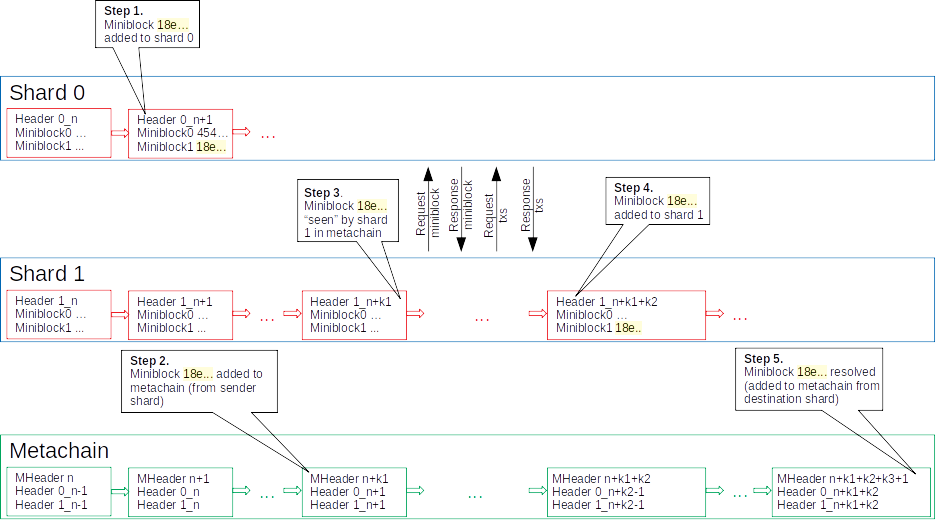
\includegraphics[width=0.9\textwidth]{shardtrans.png}
\centering
\caption{Exemple d'execució de transacció entre dos \textit{shards}. (Font: Fig. 4 de \cite{elrond2019}).}
\label{fig:shardingtrans}
\end{figure}

Observem en la \textbf{Fig. \ref{fig:shardingtrans}} un exemple de transacció asíncrona amb dos \textit{shards} implicats. Després d'arribar la transacció al \textit{shard} 0 (\textbf{\textit{step} 1}), la capçalera del bloc i els miniblocs s'envien a la \textit{metachain}. Aquesta darrera dona fe\footnote{``Donar fe'' o ``autenticar'' són les traduccions al català que he trobat més adients pel verb anglès ``to notarize''. El verb ``notarizar'' existeix en espanyol, però no existeix ``notaritzar'' en català. En qualsevol cas, empraré aquest darrer terme en algunes ocasions entre cometes per no generar confusions.} d'aquest bloc del \textit{shard} 0 creant un nou bloc a la metacadena que conté la següent informació sobre tots els miniblocs: identificador del \textit{shard} remitent, identificador del \textit{shard} receptor i \textit{hash} del minibloc (\textbf{\textit{step} 2}). El \textit{shard} 1 veu el minibloc a la \textit{metachain} i obté el seu \textit{hash} del metabloc (\textbf{\textit{step} 3}), per després demanar el minibloc al \textit{shard} 0 i executar-lo altra vegada (\textbf{\textit{step} 4}). Finalment, el \textit{shard} 1 envia el resultat a la \textit{metachain} que valida la transacció creuada (\textbf{\textit{step} 5}). En aquest punt la transacció ja es pot considerar finalitzada.

\subsection{\textit{La màquina virtual d'Elrond}}
La màquina virtual d'Elrond executa WebAssembly (Wasm)\footnote{\url{https://webassembly.org/}}, un llenguatge de baix nivell amb format binari compacte anomenat \textit{bytecode} \cite{mozilla2021}. El fet que executi Wasm implica que es puguin escriure contractes intel·ligents en qualsevol llenguatge que sigui possible compilar cap a \textit{bytecode} (C, C++, C\#, Rust, Go, TypeScript, etc.). Tot i això, Elrond recomana als desenvolupadors que emprin Rust i els hi faciliten un \textit{framework}\footnote{\url{https://github.com/ElrondNetwork/elrond-wasm-rs}} per a aquest llenguatge, així com un \textit{plugin} per a l'IDE de Microsoft Visual Studio Code\footnote{\scriptsize\url{https://marketplace.visualstudio.com/items?itemName=Elrond.vscode-elrond-ide}}. Entre les característiques a destacar de la màquina virtual d'Elrond \cite{elrond2022,mincub2020}:
\begin{itemize}
	\item \textbf{Sense estat}: Això significa que, quan un \textit{smart contract} sigui executat, es guardarà la informació en una estructura de dades transitòria, en lloc d'escriure directament en l'estat. Quan acabi l'execució, si aquesta és exitosa, l'API aplicarà els canvis a l'emmagatzematge i/o a la cadena de blocs. 
	\item \textbf{Execució fora de procés}: La màquina virtual serà executada en un procés independent i el node en si mateix en un altre, tot i que compartiran informació a través de canonades (\textit{pipes}) anònimes a memòria principal.  A més, el \textit{bytecode} s'executarà en un entorn aïllat i la memòria del procés de la màquina virtual serà inaccessible.
	\item \textbf{Motor d'execució ràpida}: Com a motor d'execució s'empra una versió modificada per Elrond de Wasmer\footnote{\url{https://wasmer.io/}}, una implementació de Wasm\footnote{Realitzada per Wasmer Inc. Aquesta empresa també ha creat un gestor de paquets que permet els desenvolupadors compartir mòduls empaquetats de codi Wasm.} de codi obert escrita en Rust per entorns servidor. Per les característiques de Wasmer, l'execució dels contractes intel·ligents es fa a una velocitat gairebé nadiua.
	\item \textbf{Trucades asíncrones entre contractes}: Els contractes intel·ligents poden executar trucades entre ells fent servir l'API de la màquina virtual. Com hem vist, la xarxa d'Elrond es fragmenta adaptativament, el que pot fer que es truqui a un \textit{smart contract} que es trobi en un altre \textit{shard}. En aquest cas l'execució serà asíncrona. Si ambdós estan en el mateix fragment, l'execució serà síncrona. Tot això es fa de forma transparent per al desenvolupador.
\end{itemize}

En el cas general, els contractes intel·ligents seran compilats generant un arxiu WASM que serà desplegat en alguna de les xarxes d'Elrond. 

\subsection{Execució de contractes intel·ligents en l'arquitectura amb \textit{shards}}

Altre punt important a destacar és l'execució dels \textit{smart contracts} en aquesta arquitectura fragmentada. Elrond ho solventa amb una solució amb execució asíncrona entre els \textit{shards} \cite{elrond2019}. 

El procés comença quan l'usuari crea una transacció per executar un contracte intel·ligent. Si el contracte intel·ligent no és ubicat en el mateix \textit{shard}, el cost de la transacció es lleva del compte del remitent i s'afegeix a un minibloc –segons correspongui a l'adreça del receptor– del seu \textit{shard}. La transacció és ``notaritzada'' per la \textit{metachain} i després processada pel \textit{shard} de destí. Al fragment de destí, la transacció es tracta com una invocació del mètode del contracte intel·ligent, ja que és on es troba (l'adreça de destí és la del \textit{smart contract}). Per a la trucada del contracte intel·ligent, es crea un compte temporal que suplanta el compte del remitent, amb el saldo del valor de la transacció i es crida el contracte intel·ligent. Després de l'execució, el contracte intel·ligent pot retornar resultats que afecten diversos comptes en diferents \textit{shards}. Els resultats que afecten els comptes del \textit{shard} del contracte intel·ligent s'executen a la mateixa ronda, en cas contrari es crearan transaccions \textit{Smart Contract Result} (SCR). En aquest darrer cas, es creen miniblocs SCR per a cada \textit{shard} de destí que posteriorment són ``notaritzats'' per la \textit{metachain} (de la mateixa manera que hem vist a la secció \ref{sec:transshards} per a les transaccions entre \textit{shards}). Finalment, són processats pels \textit{shards} respectius (on resideixen els comptes de destí). En el cas que un contracte intel·ligent truqui dinàmicament a un altre que es trobi en un \textit{shard} diferent, aquesta trucada es desaria com a resultat intermedi i es tractaria de la mateixa manera que per als comptes. Aquesta solució necessitarà \textbf{almenys 5 rondes per completar-se}, però té els avantatges de què \textbf{no es necessita cap bloqueig ni moure estats entre \textit{shards}}.

\subsection{Xarxes Elrond disponibles}\label{sub:xarxes}
En Elrond tenim tres xarxes disponibles:
\begin{itemize}
\item \textbf{\textit{Mainnet}}: És la xarxa en producció d'Elrond. És a dir, es fan transaccions reals amb  el pertinent cost econòmic. En el moment de redactar la present secció, té més de 3000 nodes validadors distribuïts en 3 \textit{shards} i en una \textit{metachain}.
\item \textbf{\textit{Devnet}}: És una xarxa pública de proves mantinguda per la comunitat d'Elrond on qualsevol desenvolupador pot provar els seus contractes intel·ligents i DApps en un entorn real. Té uns 300 nodes validadors distribuïts en 3 \textit{shards} i en una \textit{metachain}. \textbf{En el present treball empraré aquesta xarxa}, en detriment de \textit{testnet}, per tenir més estabilitat.
\item \textbf{\textit{Testnet}}: També pública i mantinguda per la comunitat d'Elrond, però s'empra per fer proves de futures millores i rendiment \cite{mincub2019-2} (això implica que el \textit{blockchain} es pot reiniciar\footnote{En el grup de Telegram ``\textit{Elrond Validators Announcements}'' (\url{https://t.me/ElrondValidatorsAnn}) es va anunciar que es faria una ronda de gènisi per la \textit{devnet} (reinici) per a dia 29 de març de 2022.}). Té uns 2000 nodes repartits en 3 \textit{shards} i en una \textit{metachain}.
\end{itemize}

\begin{figure}[!htb]
\begin{subfigure}[b]{0.32\textwidth}
  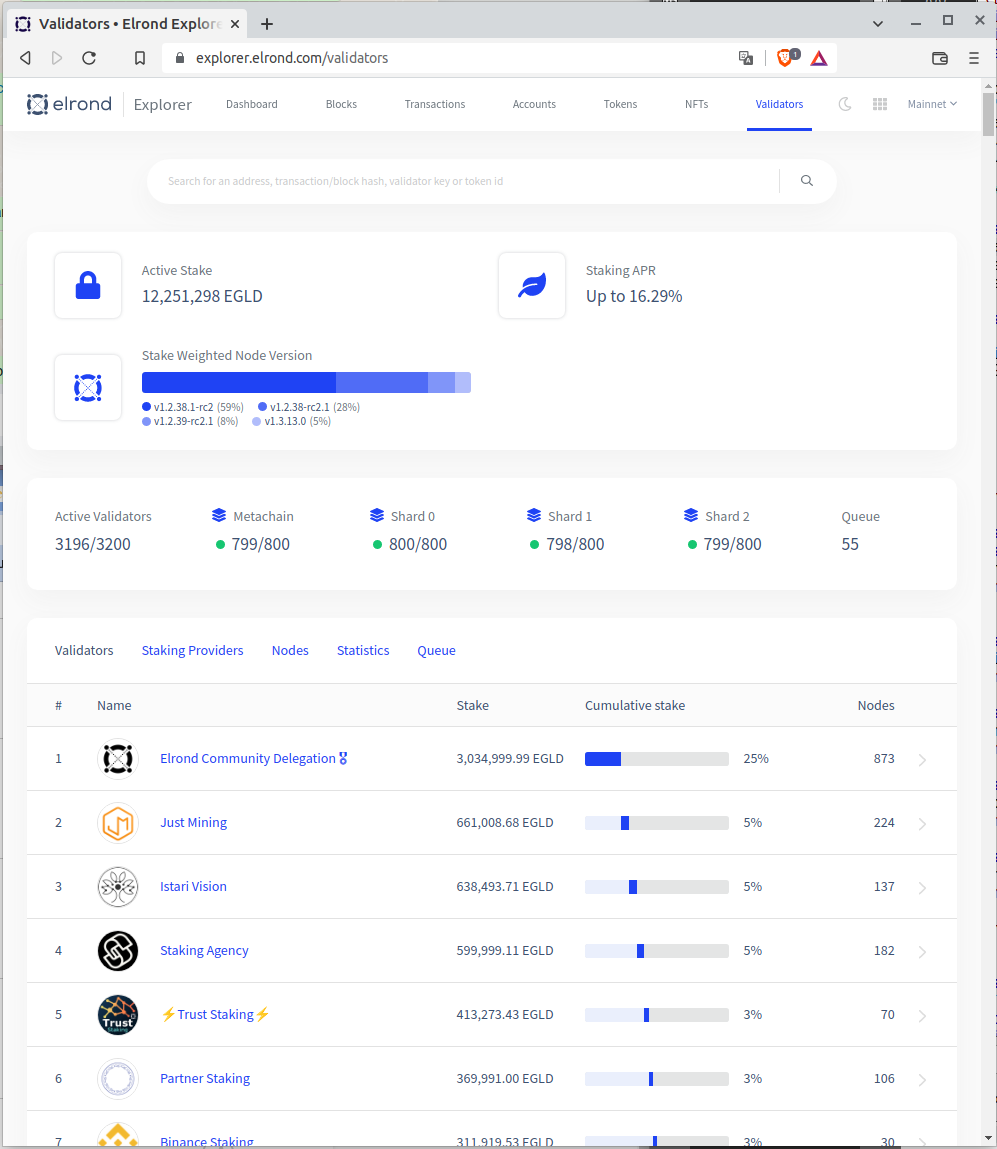
\includegraphics[width=\linewidth]{mainnet.png}
  \caption{\textit{Mainnet}: \scriptsize\url{https://explorer.elrond.com/validators}}\label{fig:mainnet}
\end{subfigure}\hfill
\begin{subfigure}[b]{0.32\textwidth}
  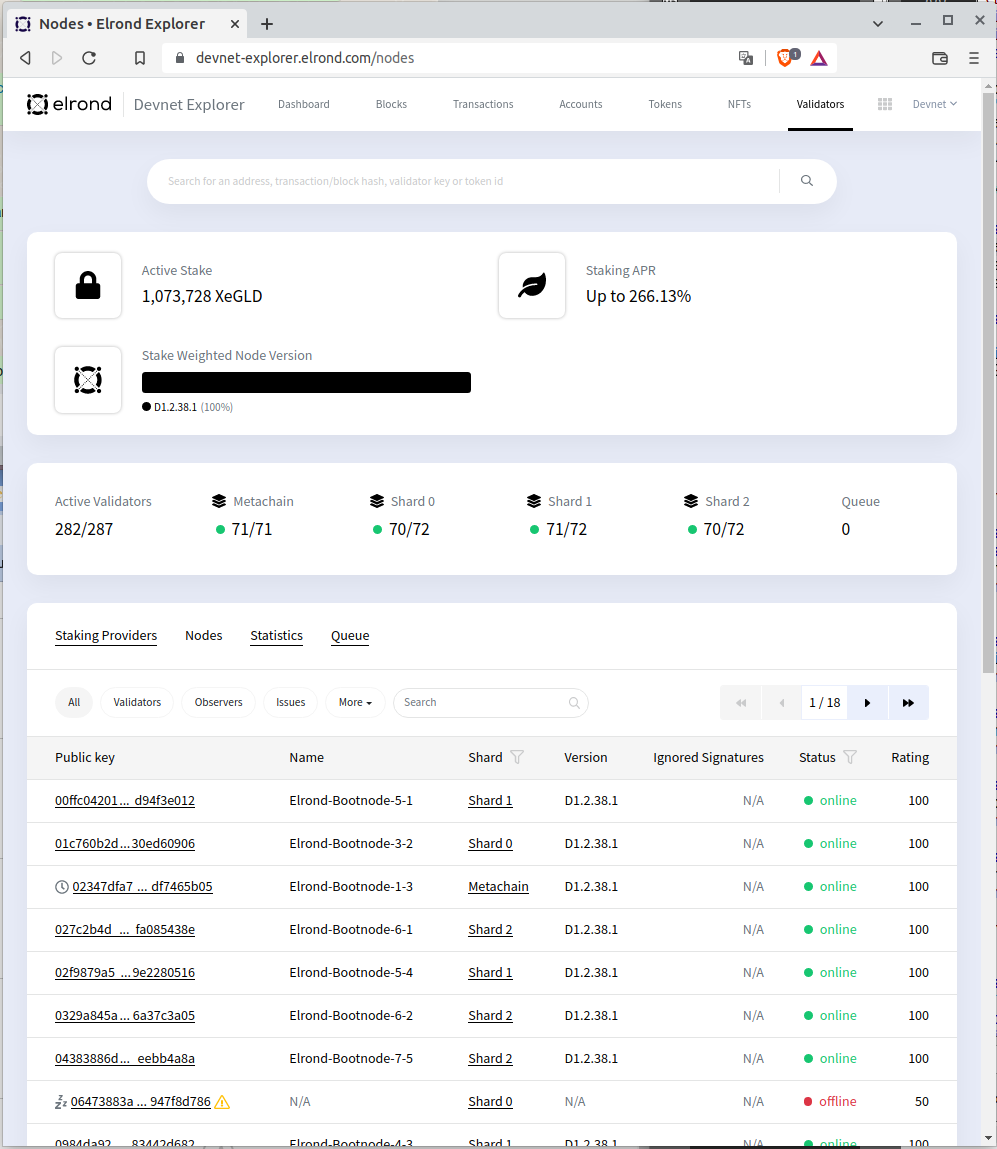
\includegraphics[width=\linewidth]{devnet.png}
  \caption{\textit{Devnet}: \scriptsize\url{https://devnet-explorer.elrond.com/nodes}}\label{fig:devnet}
\end{subfigure}\hfill
\begin{subfigure}[b]{0.32\textwidth}
  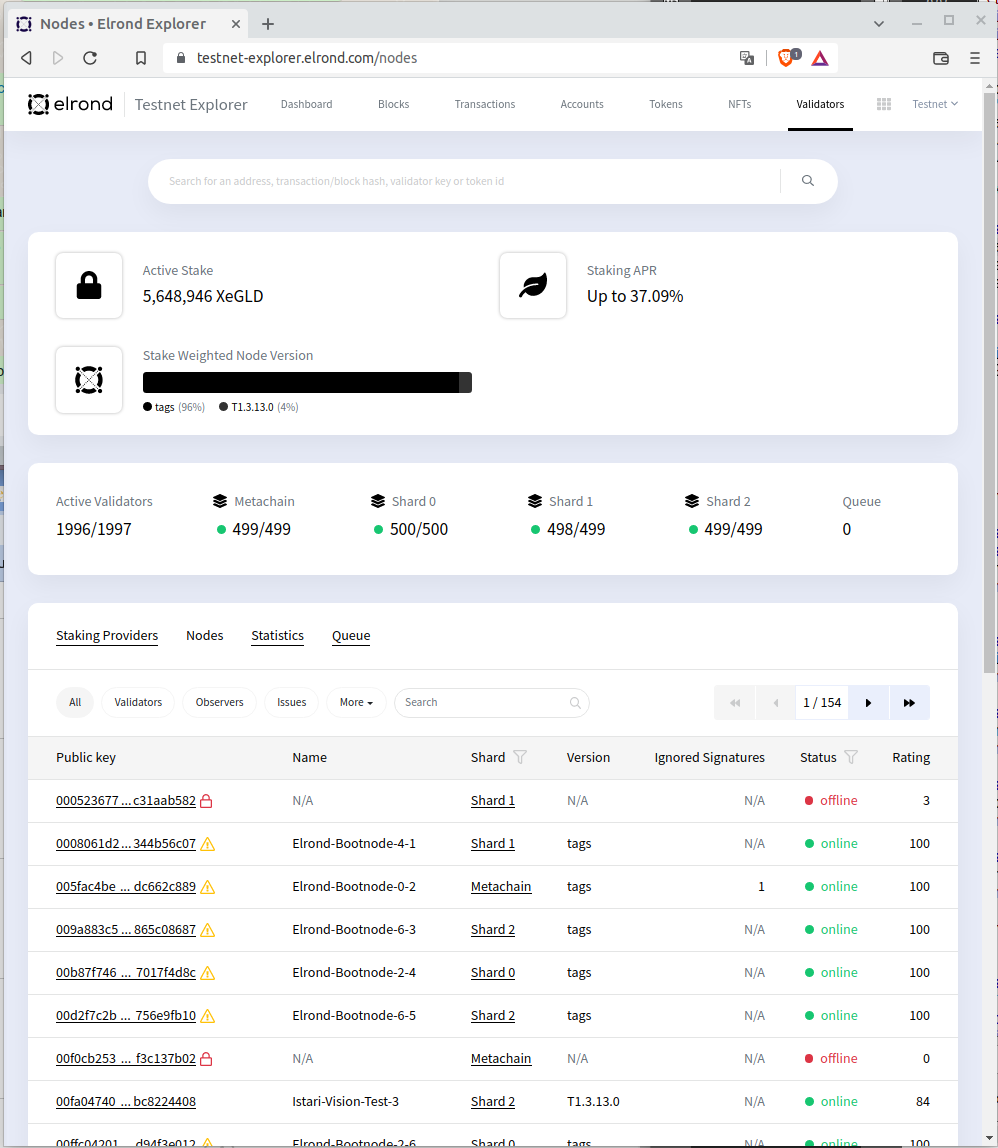
\includegraphics[width=\linewidth]{testnet.png}
  \caption{\textit{Testnet}: \scriptsize\url{https://testnet-explorer.elrond.com/nodes}}\label{fig:testnet}
\end{subfigure}\hfill
\caption{Exploradors de les xarxes disponibles a Elrond.}\label{fig:nets}
\end{figure}

\subsection{Muntar un node validador}
Com ja s'ha deixat entreveure, la \textbf{xarxa d'Elrond} és composta pels seus nodes i per la interconnectivitat entre ells. Com s'ha dit en la secció \ref{sub:entitat}, per \textbf{node} s'entendrà qualsevol instància del programari de codi obert desenvolupat per Elrond per a aquesta tasca \footnote{Programari disponible a: \url{https://github.com/ElrondNetwork/elrond-go}.}. A més a més, qualsevol persona o entitat responsable de la gestió d'un o més d'aquests nodes es coneix com a ``\textbf{operador de nodes}''. Com també s'ha vist, la xarxa és dissenyada per ser segura i per poder balancejar la seva càrrega. Així, quan un nou node s'uneix a la xarxa aporta més seguretat i eficiència. I la xarxa premiarà els nodes per la seva aportació, creant-se així una espècie de simbiosi.

\textbf{Elrond és una xarxa descentralitzada de \textit{blockchain}}, és a dir, nodes de procedència desconeguda s'uneixen per crear seqüencialment blocs amb una cadència determinada. Els blocs contenen operacions que es realitzaren a petició dels usuaris de la xarxa pagant unes taxes (\textit{fees}) per l'execució d'aquestes. Entre les operacions es troben la transferència de \textit{tokens} entre comptes o l'execució de contractes intel·ligents (totes les operacions prenen la forma de transaccions). Per tant, es defineix així un llibre de comptabilitat distribuït que no depèn de cap entitat central. 

Els nodes que estan autoritzats a prendre part en l'algorisme de consens s'anomenen \textbf{validadors}. Com que són els que veritablement produeixen i validen blocs, són els únics nodes recompensats amb EGLD per la seva contribució. Com ja vàrem dir en la secció \ref{sub:entitat}, per assegurar el bon comportament dels validadors han de tenir bloquejats 2500 EGLD (\textit{stake}). Els nodes sense \textit{stake} s'anomenen \textbf{observadors} (no participen en el consens i no guanyen recompenses). Si el validador no funciona correctament (desconnexions de la xarxa en mig del procés de consens, accions malicioses, etc.) serà ``multat'' perdent EGLD (\textit{stake slashing}) o fins i tot, en casos greus, se li llevarà l'estatus de validador (el node passarà a l'estat ``\textit{jailed}'' i no es triarà per al consens si no paga una multa de 2,5 EGLD).  Si això succeeix també davallarà la seva qualificació (\textit{rating score}). Com que aquesta puntuació defineix la fiabilitat del validador, serà considerada per l'algorisme de selecció de nodes per triar el grup de consens. Així, s'afavoreix l'elecció de nodes amb qualificacions altes, també se'ls hi premiarà amb més EGLD. 

Els requisits mínims del sistema són:
\begin{itemize}
\item 4 CPU dedicades (Intel/AMD amb \textit{flags} SSE4.1 i SSE4.2 activats).
\item 8 GB de RAM.
\item Disc dur SSD amb 200 GB d'espai lliure.
\item Connexió a Internet de 100 Mbit/s sempre activa (mínim 4 TB/mes).
\item Sistema operatiu Linux\footnote{Es recomana Ubuntu 20.04.}/MacOS.
\end{itemize}

Com podem observar, són característiques d'un PC/Mac convencional en l'actualitat (i no d'ordinadors amb potents targetes gràfiques dedicades com passa amb el PoW de Bitcoin). No és l'objectiu del present treball, però guies com-es-fa\footnote{Traducció del Termcat del terme ``\textit{howto}''.} per instal·lar el programari per muntar un node validador en la xarxa Elrond es poden trobar a \cite{elrond2022} o \cite{penalver2019}.\footnote{Aquesta secció torna a ser una síntesi de l'apartat ``\textit{Validators}'' de \cite{elrond2022}.}

\subsection{Carteres}
Com ja s'ha comentat en la secció \ref{sub:context} existeixen diferents carteres que es poden fer servir per enviar, rebre i emmagatzemar EGLD de forma segura.
\begin{itemize}
\item \textbf{Moneder web}. Existeix una versió per a cadascuna de les xarxes:\footnote{Per a la \textit{devnet} i la \textit{testnet} es disposa d'una opció ``\textit{Faucet}'' per obtenir xEGLD (que no té cap cost en moneda \textit{fiat} i et permetrà poder relalitzar transaccions).}
	\begin{itemize}
	\item \textit{Mainnet}: Accesible a \url{https://wallet.elrond.com/}.
	\item \textit{Devnet}: Accesible a \url{https://devnet-wallet.elrond.com/}.
	\item \textit{Testnet}: Accesible a \url{https://testnet-wallet.elrond.com/}.
	\end{itemize}
Tampoc és l'objectiu del present treball explicar com crear un moneder, però una guia com-es-fa es pot trobar en \cite{elrond2022}. Quan es crea s'haurà d'introduir una contrasenya\footnote{Ha de tenir almenys nou caràcters, una lletra majúscula, un símbol i un nombre.} i se'ns donaran 24 paraules secretes (que permeten generar la clau privada). El procés finalitzarà descarregant un fitxer json (\textit{keystore file}). Com es veu en la Fig. \ref{fig:webwallet}, podem accedir al nostre moneder amb aquest arxiu json i introduint la contrasenya que hem creat (nombre 1 en la Fig. \ref{fig:webwallet}). Una altra opció és generar un fitxer ``PEM'' (\textit{Privacy Enhanced Mail}) amb la nostra clau privada i emprar-lo per accedir (nombre 3 en la Fig. \ref{fig:webwallet}), que es pot generar emprant la utilitat d'Elrond ``\textit{erdpy}'' (s'hauran d'introduir les 24 paraules secretes separades per un espai):
\begin{lstlisting}[
    basicstyle=\footnotesize,
]
erdpy --verbose wallet derive testdev-wallet.pem --mnemonic
\end{lstlisting}
Finalment, es pot iniciar sessió amb un moneder de maquinari (per exemple amb un Ledger Nano S) o llegint un codi QR amb l'aplicació mòbil Maiar (nombres 2 i 4 en la Fig. \ref{fig:webwallet}, respectivament).
\begin{figure}[h]
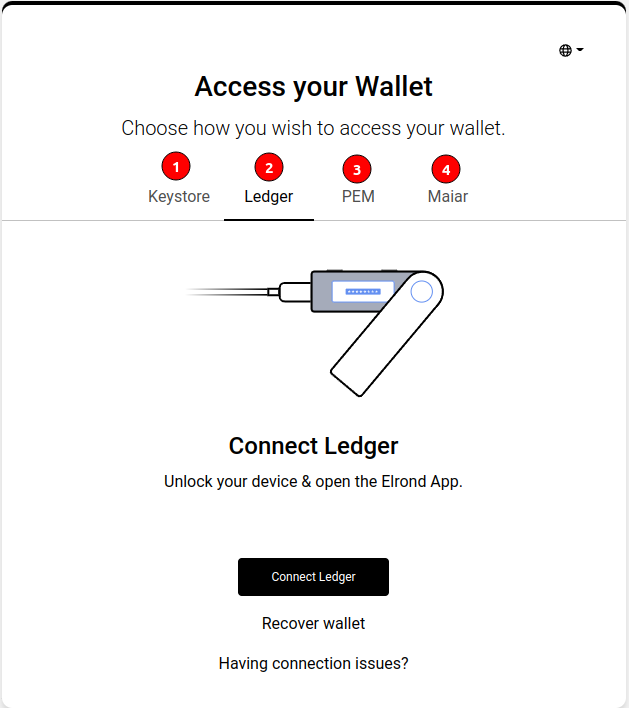
\includegraphics[width=0.5\textwidth]{webwallet.png}
\centering
\caption{Mètodes d'accés al moneder web.}\label{fig:webwallet}
\end{figure} 
\item \textbf{Maiar DeFi Wallet}. Es tracta d'una extensió per a navegadors de la família de Chrome\footnote{\url{https://chrome.google.com/webstore/detail/maiar-defi-wallet/}}. El funcionament i prestacions és similar al moneder web (fent la comparació amb la xarxa Ethereum, seria com l'extensió ``Metamask''\footnote{\url{https://metamask.io/}}). En la Fig. \ref{fig:maiarwalletb} es pot comprovar que també es pot canviar entre les tres xarxes disponibles (llista desplegable a dalt a la dreta que diu ``Main'').
\begin{figure}[!htb]
\begin{subfigure}[b]{0.4\textwidth}
  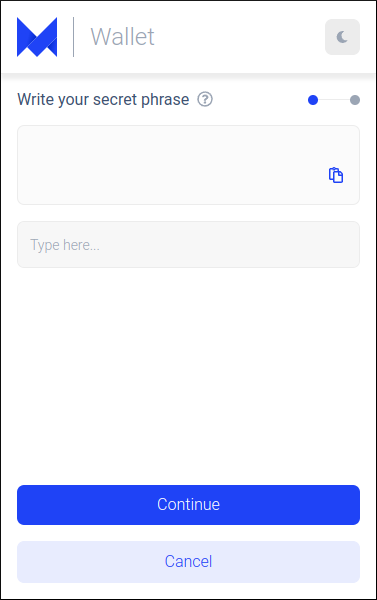
\includegraphics[width=\linewidth]{maiarextensio.png}
  \caption{}\label{fig:maiarwalleta}
\end{subfigure}\hfill
\begin{subfigure}[b]{0.4\textwidth}
  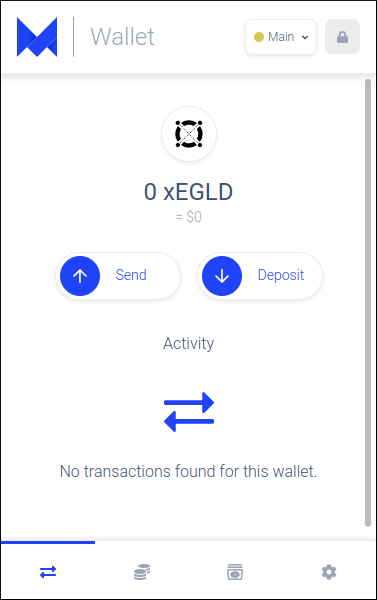
\includegraphics[width=\linewidth]{maiarextensio2.png}
  \caption{}\label{fig:maiarwalletb}
\end{subfigure}\hfill
\caption{Maiar DeFi Wallet.}\label{fig:maiarwallet}
\end{figure}
\item \textbf{\textit{Maiar}}\footnote{\url{https://maiar.com/}}. DApp que implementa una cartera digital per dispositius iOS i Android. Permet enviar o rebre diners emprant el número de telèfon mòbil o un \textit{herotag} (una espècie de nom d'usuari que es pot emprar en lloc de la teva adreça). És completament descentralitzada, sense custòdia i Elrond no té accés als fons de l'usuari en cap moment. Es pot treballar amb criptoactius com Elrond Gold (EGLD), Binance (BNB), Ethereum (ETH) o Bitcoin (BTC). Com no pot ser d'altra forma, es disposen de mecanismes de recuperació (una frase) per rescatar els fons en cas de pèrdua o robatori del nostre telèfon intel·ligent. No he trobat forma de connectar a la \textit{devnet} o \textit{testnet} des de Maiar, penso que déu ser així perquè és principalment dissenyada per treballar amb la \textit{mainnet}. Òbviament, aquesta DApp és pensada per comprar criptoactius a través de pagaments amb targeta bancària o transferències SEPA (s'han d'emprar passarel·les en ambdós casos). Curiosament, no permet fer \textit{swaps} entre criptoactius (només es poden fer des de Maiar Exchange).
\begin{figure}[h]
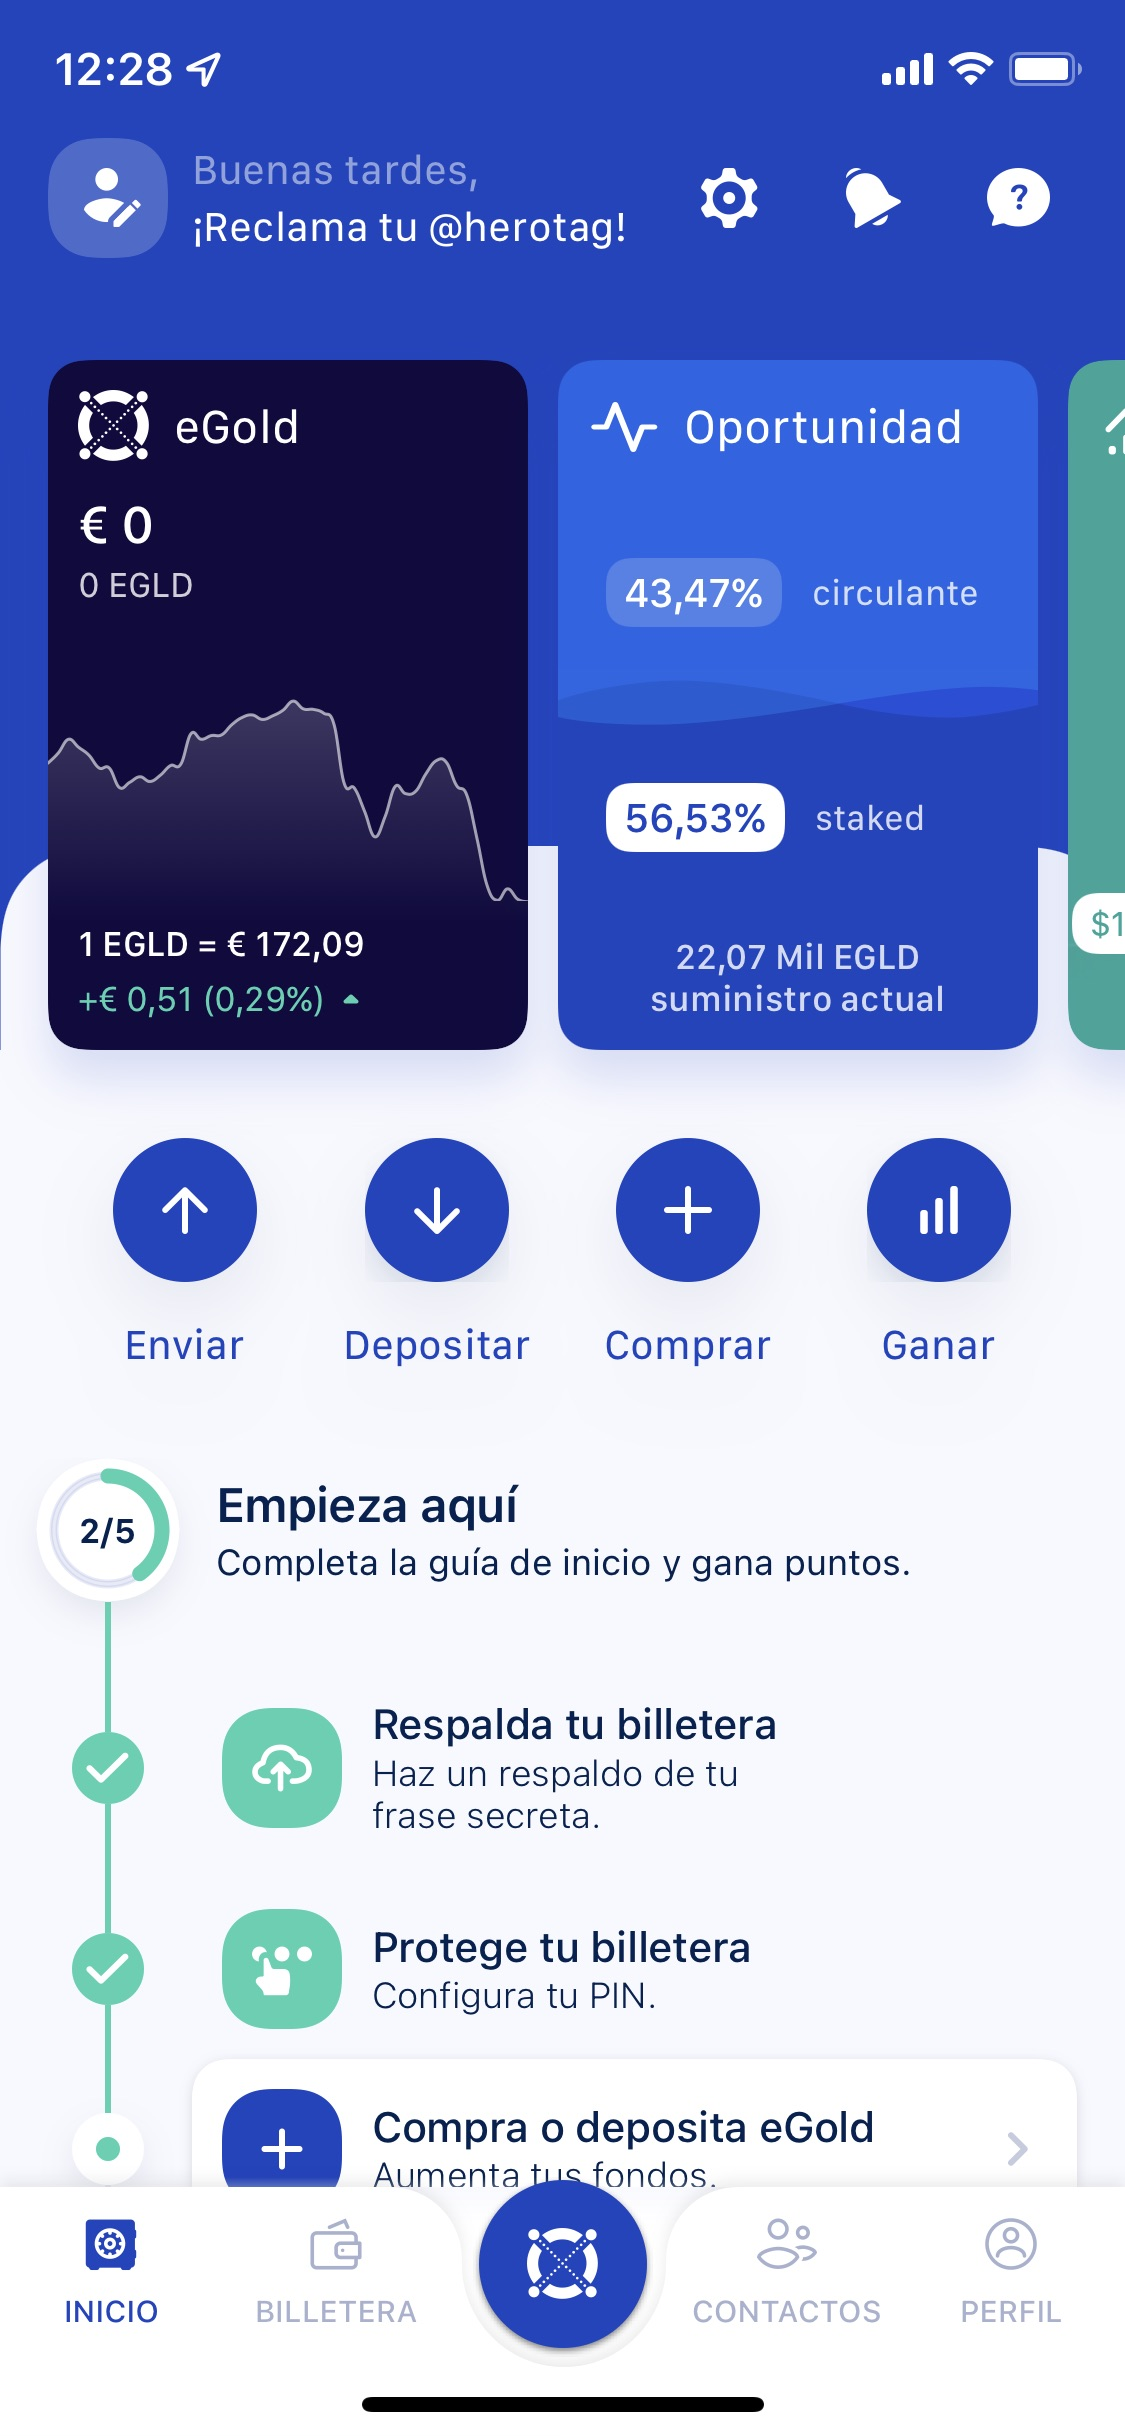
\includegraphics[width=0.3\textwidth]{maiarapp.png}
\centering
\caption{Maiar per iPhone.}\label{fig:maiarapp}
\end{figure} 
\item \textbf{\textit{Webhooks}}. Són enllaços que criden\footnote{En català balear fem ús del verb ``cridar'' en lloc del verb ``trucar''. Així diem per exemple ``cridar per telèfon'' o ``cridar el mètode d'un objecte''.} a la cartera de l'usuari perquè iniciï sessió o ompli un formulari per realitzar una transacció de pagament amb els arguments proporcionats. Un cop realitzada l'acció, l'usuari és redirigit a un URL amb informació d'estat d'èxit o d'error. Un exemple seria \cite{elrond2022}:
\begin{lstlisting}[
    basicstyle=\scriptsize,
]
https://wallet.elrond.com/hook/login?callbackUrl=https://example.com/
\end{lstlisting}
\item \textbf{\textit{Ledger}}. És l'opció recomanada per Elrond si es fa feina amb grans quantitats d'EGLD. Podem emmagatzemar els nostres criptoactius en moneders de maquinari com són els dispositius \textit{Ledger Nano S} o \textit{Ledger Nano X}.
\end{itemize}

\subsection{Maiar Exchange}\label{subsec:maiarexchange}
Maiar Exchange\footnote{\url{https://maiar.exchange/}} és un DEX (\textit{Decentralized EXchange}) basat en \textit{liquidity pools} –fons de liquiditat– creat per Elrond emprant la seva arquitectura escalable. Permet els usuaris efectuar la compravenda de criptoactius (\textit{trading}). A més a més, els usuaris poden convertir-se en proveïdors de liquiditat aportant els seus actius (guanyant \textit{tokens} MEX per cada transacció d'intercanvi realitzada segons el parell de \textit{tokens} aportats com a reserva). MEX és el \textit{token} nadiu de Maiar Exhange. A part de tenir la funció d'incentivar els usuaris perquè proporcionin liquiditat, també serà emprat en processos de governança. Així, ens trobem davant d'un Exchange de \textit{criptoactius} sense intermediaris, cosa que abarateix els costos de les transaccions i dels \textit{swaps}.

Entre el que podem fer amb Maiar Exchange vull destacar \cite{everstake2021,elrond2021}:
\begin{itemize}
\item \textbf{\textit{Swapping}} (intercanvi): Consisteix a intercanviar un criptoactiu per un altre. El mecanisme d'intercanvi consisteix en permutar els actius de l'usuari amb els \textit{liquidity pools} (fons de liquiditat), i no directament amb altres participants en el mercat. Els preus dels actius es fixen a partir d'una fórmula matemàtica del que s'anomena \textit{Automated Market Making}. En lloc d'utilitzar un llibre de comptabilitat com en un intercanvi tradicional, els actius tenen uns preus calculats segons un algorisme. Elrond empra la fórmula \(x * y = k\), on \(x\) és la quantitat d'un token al \textit{liquidity pool} i \(y\) és la quantitat de l'altre. \(k\) és una constant fixa, el que significa que la liquiditat total del grup sempre romandrà en la mateixa proporció. Hi ha una comissió del 0,3\% per intercanviar tokens (el 0,25\% pels proveïdors de liquiditat proporcional a la seva contribució a les reserves de liquiditat i amb la resta es compraran MEX que es cremaran). En la data de redacció d'aquesta secció, els actius amb els que es poden fer intercanvis són MEX, USDC, RIDE, CRU, ZPAY, ISET, AERO, EFFORT i WAM contra  EGLD. Això significa que hi ha fons de liquiditat MEX-EGLD, USDC-EGLD, etc.
\item \textit{\textbf{Liquidity Pools}}:  Són reserves de tokens que es troben en contractes intel·ligents del DEX i estan disponibles perquè els usuaris facin intercanvis. Aquests tokens els proporcionen proveïdors de fons de liquiditat amb els quals els usuaris de la plataforma poden negociar. Els proveïdors són incentivats amb recompenses (tokens MEX) pels intercanvis que es produeixen en els seus \textit{pools} (segons s'ha explicat en el punt anterior). S'ha de destacar que els proveïdors de liquiditat en qualsevol moment poden retirar els fons que han dipositat (independentment de les condicions del mercat).  
\item \textit{\textbf{Farming}}\footnote{No m'he atrevit a traduir aquest terme, però un mot que m'agrada del català és ``conrear''.}: Consisteix en el fet que els usuaris bloquegin la seva liquiditat per obtenir recompenses. Si posem els nostres actius en un \textit{liquidity pool} obtindrem les recompenses descrites en els apartats anteriors (això és el \textit{\textbf{farming}} i és el que s'ha descrit en el punt d'adalt). Però hi ha també l'opció de posar els nostres \textit{liquidity pools} en \textit{\textbf{staking}}, el que significa que no els podrem retirar durant un temps definit a canvi d'aconseguir una recompensa major.
\end{itemize}

\begin{figure}[h]
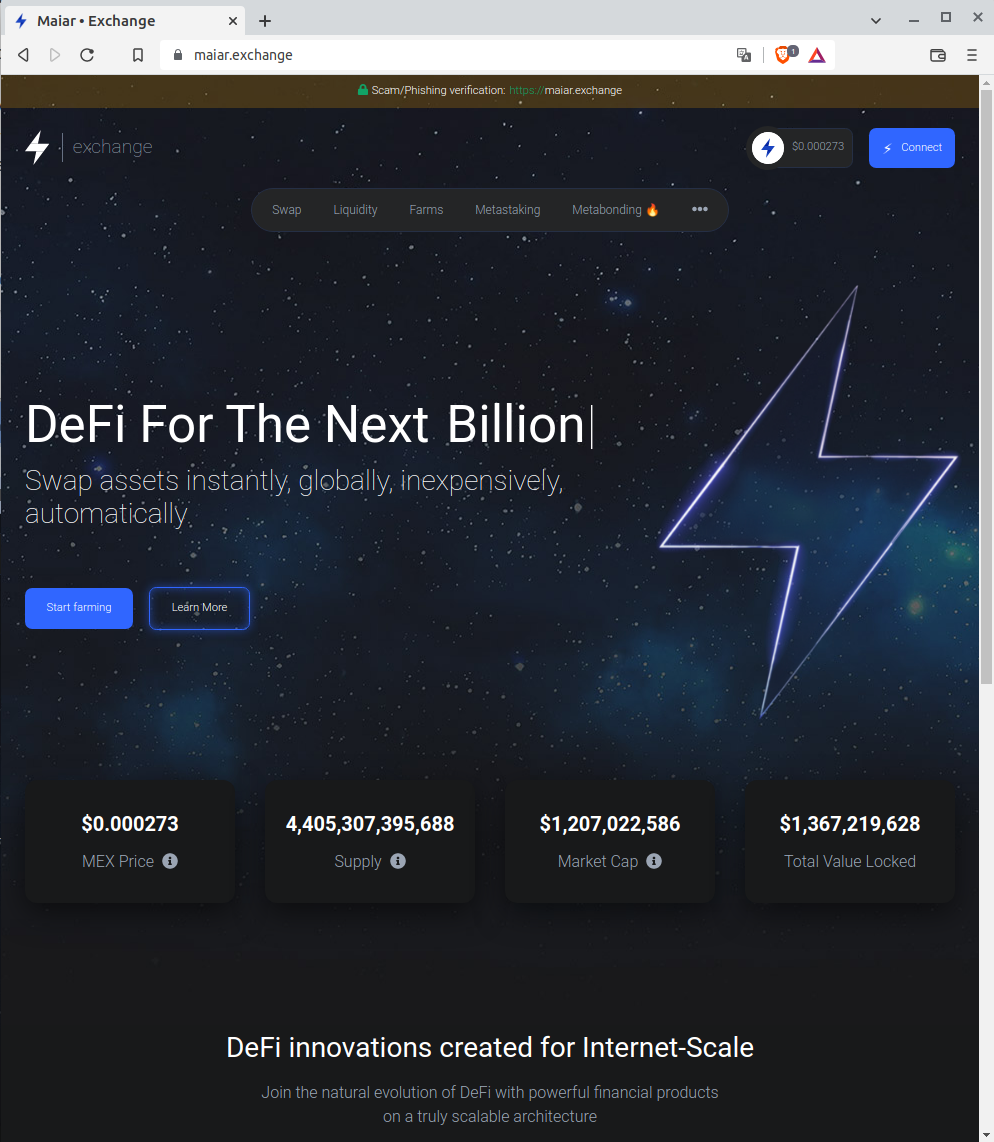
\includegraphics[width=0.75\textwidth]{maiardex.png}
\centering
\caption{Maiar Exchange.}\label{fig:maiardex}
\end{figure} 

\subsection{Altres punts destacables}\label{sub:altres}
\begin{itemize}
\item \textbf{Camps d'una transacció}:

Els camps d'una transacció sense signar en la xarxa Elrond són \cite{elrond2022}:
\begin{itemize}
\item \textbf{nonce} (\textit{number}): Nombre de seqüència del compte. És obligatori.
\item \textbf{value}	(\textit{string}): El valor a transferir. És obligatori (pot ser 0).
\item \textbf{receiver} (\textit{string}): Adreça del receptor (format \textit{bech32}). És obligatori.
\item \textbf{sender} (\textit{string}): Adreça del remitent (format \textit{bech32}). És obligatori.
\item \textbf{gasPrice} (\textit{number}): El preu del \textit{gas} que s'utilitzarà en la transacció. És obligatori.
\item \textbf{gasLimit} (\textit{number}): El nombre màxim d'unitats de \textit{gas} assignades per a la transacció. És obligatori.
\item \textbf{data} (\textit{string}): Informació arbitrària sobre la transacció, codificada en base64 . No és obligatori.
\item \textbf{chainID} (\textit{string}): Identificador de cadena. `D' per a la xarxa \textit{devnet}, `T' per a \textit{testnet} i `1' per a la \textit{mainnet}. És obligatori.
\item \textbf{version} (\textit{number}): La versió de la transacció (p. ex. 1). És obligatori.
\end{itemize}
En les transaccions que han de ser signades, amb la clau pública del remitent (amb l'algorisme Ed2519), s'ha d'afegir el següent camp: 
\begin{itemize}
\item \textbf{signature} (\textit{string}): Signatura digital que consta de 128 caràcters hexadecimals (64 bytes en representació en brut).
\end{itemize}
Hi ha disponibles diferents eines per realitzar la signatura des de la \textit{shell} de Linux i des del codi font: \textit{erdpy}, \textit{erdwalletjs-cli} o \textit{elrond-core-js}.
\item \textbf{Decimals per treballar amb EGLD}: Un EGLD és configurat per tenir 18 decimals. Així, per exemple 2,5 EGLD tendrien un valor de \(2,5 * 10^{18} = 2500000000000000000\) wei (seguint l'estàndard de 18 decimals dels tokens ERC20). L'usuari quan creï tokens ESDT podrà definir el seu nombre de decimals (amb un màxim de 18).
\item \textbf{Costos de processament} \cite{elrond2022}:
Una transacció en la xarxa Elrond té un cost de processament (\textit{processing cost}), que s'expressa com una quantitat d'unitats de \textit{gas}. Quan es llança una transacció s'ha de proporcionar un \textit{gasLimit}, que és el cost màxim que estem disposats a assumir. El \textbf{consum real de gas} (\textit{actual gas consumption} o també \textit{used gas}) és la quantitat real que s'ha consumit del \textit{gasLimit} requerida perquè la xarxa processi la transacció. Per calcular aquest darrer, la xarxa el divideix en dos components d'utilització del \textit{gas} \cite{elrond2022}:
\begin{itemize}
\item \textbf{Moviment de valors i tractament de dades}: Això seria per exemple una transferència d'EGLD entre adreces. El cost es calcula amb la fórmula:
\begin{lstlisting}[
    basicstyle=\tiny,
]
tx.gasLimit = 
    networkConfig.erd_min_gas_limit + 
    networkConfig.erd_gas_per_data_byte * lengthOf(tx.data)
Nota:
networkConfig.erd_min_gas_limit <= tx.gasLimit i
tx.gasLimit <= networkConfig.erd_max_gas_per_transaction
\end{lstlisting}
\item \textbf{Execució de contracte intel·ligent}: Una trucada a un \textit{smart contract} requeriria aquest i l'anterior. El cost és més difícil de determinar, ja que depèn del codi font concret del contracte intel·ligent. Es solen emprar simulacions i estimacions.
\end{itemize}
Finalment, la \textbf{tarifa de processament} (\textit{processing fee}) es calcula amb respecte de l'\textit{actual gas consumption} i dels seus dos components. Per a un moviment de valors i tractament de dades s'especifica en la transacció un \textit{gas price per gas unit} (que ha de ser igual o superior al paràmetre de la xarxa \(erdmin\textunderscore  gas\textunderscore price\)). Per a l'execució d'un contracte intel·ligent el \textit{gas price per gas unit} es calcula respecte a un altre paràmetre de xarxa anomenat \(erd\textunderscore gas\textunderscore price\textunderscore modifier\):
\begin{lstlisting}[
    basicstyle=\tiny,
]
value_movement_and_data_handling_price_per_unit = tx.GasPrice
contract_execution_price_per_unit =
		tx.GasPrice * networkConfig.erd_gas_price_modifier
\end{lstlisting}

\item \textbf{ESDT (\textit{Elrond Standard Digital Token})}: La xarxa Elrond admet de forma nadiua l'emissió de \textit{tokens} creats pels usuaris (des de codi, des d'un contracte intel·ligent o des de la \textit{web wallet}). Això implica que no és necessari emprar contractes com els de tipus ERC20 de la xarxa Ethereum. Ja que el suport és nadiu, no es requereix processament extra per part de la màquina virtual (amb el que són tan eficients com el mateix EGLD).

\item \textbf{NFT (\textit{Non-Fungible Token}) i SFT (\textit{Semi-Fungible Token})}: Suport nadiu d'NFT i SFT afegint metadades i atributs a sobre de l'ESDT. Així, són bastant similars a aquests darrers però amb atributs extra (\textit{NFT Name}, \textit{Quantity}, \textit{Royalties}, \textit{Hash}, \textit{Attributes} i \textit{URI}).

\item \textbf{\textit{Local Testnet}}: Es pot configurar una \textit{testnet} en local per fer proves i \textit{debugging} del codi. Es pot emprar amb l'eina \textit{erdpy} i conté nodes validadors, nodes observadors, un \textit{seed node} i un \textit{Elrond Proxy}.

\item  \textbf{API REST}: Té dues capes a les quals es pot accedir públicament:
\begin{itemize}
\item \textbf{https://gateway.elrond.com}: La de més baix nivell. Gestiona l'encaminament de les peticions de forma transparent segons els mecanismes de fragmentació que s'han descrit en els apartats anteriors.
\item \textbf{https://api.elrond.com}:  La de més alt nivell (empra els serveis de la capa anterior). Aporta serveis com un mecanisme de memòria cau, cerques històriques amb Elasticsearch\footnote{\url{https://www.elastic.co/}}, etc.
\end{itemize}
\end{itemize}

\clearpage

\section{testDEX}\label{sec:testdex}

\subsection{Anàlisi}
\subsubsection{DEX i AMM}\label{subsub:dexamm}

Un \textbf{\textit{Decentralized exchange} (DEX)} és un mercat on els negociants de criptomonedes fan transaccions directament entre ells –d'igual a igual (\textit{peer-to-peer})– sense haver de lliurar la gestió dels seus fons a un intermediari \cite{cointelegraph}. És a dir, són dissenyats per eliminar qualsevol autoritat de supervisió en els intercanvis (\textit{swaps}) de criptoactius, evitant que s'hagin d'enviar dades de caràcter personal (noms, adreces, etc.). Per executar les ordres d'intercanvi sense intermediaris s'empren contractes intel·ligents. Això xoca amb el concepte de \textit{\textbf{Centralized exchange}} on la gestió és responsabilitat d'una organització, com ara un banc o qualsevol altra corporació, que requerirà que els seus usuaris estiguin identificats i que custodiaran els actius d'aquests (òbviament cercant un benefici econòmic).
 
En el present treball ens centrarem en una versió simplificada de DEX fent servir \textit{Automated Market Makers} (AMM). Els diferents tipus de DEX es poden observar en la figura \ref{fig:dextypes}.
\begin{figure}[h]
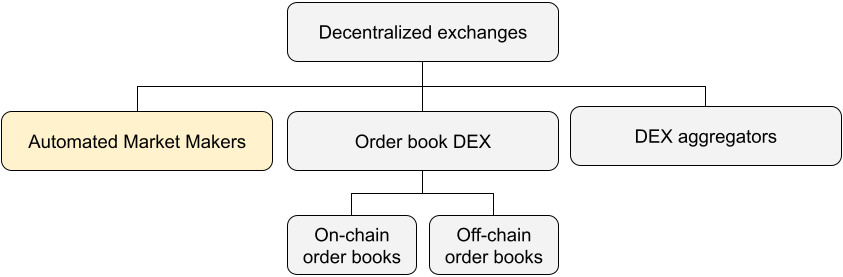
\includegraphics[width=0.95\textwidth]{DEXtypes.png}
\centering
\caption{Tipus de DEX. (Font: \cite{cointelegraph}).}\label{fig:dextypes}
\end{figure} 

En \cite{delarosa} es descriu que una de les formes de prescindir del llibre d'ordres d'un \textit{Exchange} tradicional és emprant AMM. Aquests protocols fan servir una fórmula matemàtica per calcular el preu dels actius d'un fons de liquiditat segons l'estat d'aquest (tal qual hem vist en la secció \ref{subsec:maiarexchange}). Quan es vulgui fer un intercanvi entre criptoactius s'interactuarà directament amb un contracte intel·ligent que determinarà el preu de compra de l'actiu destí segons l'estat del fons de liquiditat. La fórmula per calcular això, també vista en la secció \ref{subsec:maiarexchange}, és:
\[x * y = k\]
Amb \(x\) la quantitat d'un token al fons de liquiditat, \(y\) la quantitat de l'altre i \(k\) una constant fixa per mantenir la proporcionalitat entre el parell de \textit{tokens}.

Imaginem que volem intercanviar una quantitat del primer token \(t_x\) i volen conèixer la quantitat \(t_y\) que rebrem a canvi:
\[(x + t_x) * (y - t_y) = k\]
\[(y - t_y) = \frac{k}{x + t_x}\]
\[t_y = y - \frac{k}{x + t_x}\]
\[t_y = \frac{y * x + y * t_x - k}{x + t_x}\]
\[t_y = \frac{y * t_x}{x + t_x}\]

Si per contra volem donar \(t_y\) i rebre \(t_x\):
\[(x - t_x) * (y + t_y) = k\]
\[(x - t_x) = \frac{k}{y + t_y}\]
\[t_x = x - \frac{k}{y + t_y}\]
\[t_x = \frac{x * y + x * t_y - k}{y + t_y}\]
\[t_x = \frac{x * t_y}{y + t_y}\]

Aquesta situació seria utòpica ja que no se pagaria cap taxa (\textit{fee}). Si afegim una comissió, les fórmules d'abans quedarien de la següent forma:
\[t'_x = x - \frac{k}{y + t_y * (1 - fee)} = \frac{x * y + x * t_y *(1 - fee) - k}{y + t_y * (1 - fee)}\]
\[t'_x = \frac{x * t_y *(1 - fee)}{y + t_y * (1 - fee)}\]
\[t'_y = y - \frac{k}{x + t_x * (1 - fee)} = \frac{y * x + y * t_x * (1 - fee) - k}{x + t_x * (1 - fee)}\]
\[t'_y = \frac{y * t_x * (1 - fee)}{x + t_x * (1 - fee)}\]

Així, si es realitzes el \textit{swap}, el que quedaria acumulat en el contracte intel·ligent seria:
\[acumulat_x = t_x - t'_x\]
\[acumulat_y = t_y - t'_y\]

Per exemple, imaginem que tenim un fons de liquiditat amb el parell xEGLD-UOC –``UOC'' és un ESDT creat per mi– amb 10 xEGLD\footnote{En el present treball empraré indistintament els termes EGLD i xEGLD. En qualsevol cas, ha de quedar clar que EGLD es fa servir en la mainet (té un cost econòmic) i xEGLD es fa servir en la devnet/testnet.}  (\(x\)) i 10000 UOC (\(y\)). Així tenim que la constant \(k\) queda com:
\[k = x * y = 10 * 10000 = 100000\]


Suposem també que volem canviar 1 xEGLD (\(t_x\)) per UOC (\(t_y\)) i que hi ha una comissió del 0,5\%:
\[t_y = \frac{y * t_x}{x + t_x} = \frac{10000 * 1}{10 + 1} = 909,090909091\]

\[t'_y = \frac{y * t_x * (1 - fee)}{x + t_x * (1 - fee)} = \frac{10000 * 1 * (1 - 0,005)}{10 + 1 * (1 - 0,005)} = 904,956798545\]

\[acumulat_y = t_y - t'_y = 909,090909091 - 904,956798545 = 4,134110546\]

\[k = (x + t_x) * (y - t_y) = (10 + 1) * (10000 - 909,090909091) =\]
\[= 11 * 9090,909090909 = 99999,999999999\]

Si seguim i ara canviem 1000 UOC (\(t_y\)) per xEGLD (\(t_x\)):
\[t_x = \frac{x * t_y}{y + t_y} = \frac{11 * 1000}{9090,909090909 + 1000} = 1,09009009 \]
\[t'_x = \frac{x * t_y *(1 - fee)}{y + t_y * (1 - fee)} = \frac{11 * 1000 *(1 - 0,0005)}{9090,909090909 + 1000 * (1 - 0,0005)} =\]
\[= 1,089599034\]
\[acumulat_x = t_x - t'_x = 1,09009009 - 1,089599034 = 0,000491056\]

\[k = (x - t_x) * (y + t_y) = (11 - 1,09009009) * (9090,909090909  + 1000) =\]
\[= 9,90990991 * 10090,909090909 = 100000,000000908\]

A tot això se li ha d'afegir una cosa més: \textbf{la comissió que pagarà l'usuari a la xarxa Elrond}. En la secció \ref{sub:altres} s'ha vist que emprar la xarxa Elrond duu associat uns costos pel moviment de valors i tractament de dades (transferim una quantitat de tokens al contracte intel·ligent) i per execució de contracte intel·ligent (el \textit{smart contract} que implementa l'AMM). Això encarirà l'operació a l'usuari, ja que el codi que s'executa dins aquest contracte influirà en el cost.

Finalment, es pot observar que \textbf{l'arrodoniment provoca que la constant \(k\) es vagi desviant del seu valor original}. El codi del contracte intel·ligent hauria de corregir aquest problema.

\subsubsection{Les variants de DEX i AMM a testDEX}
Per assolir els objectius del projecte no fa falta arribar a desenvolupar un DEX de l'estil de Maiar Exchange, Uniswap\footnote{\url{https://uniswap.org/}} o PancakeSwap\footnote{\url{https://pancakeswap.finance/}}. Òbviament, un projecte d'aquesta envergadura seria poc realista per una limitació clara de temps. Per exemple, el protocol AMM no és exempt de problemes que s'haurien de tractar \cite{vuterin2018}. Així, en aquesta versió inicial faré una sèrie d'adaptacions per ajustar-me al temps disponible:
\begin{itemize}
\item El propietari del contracte intel·ligent serà l'únic que pot definir \textit{liquidity pools}.
\item El propietari del contracte serà, per tant, l'únic que rebi les comissions pels \textit{swaps}.
\item Tots els parells tindran com a un dels seus components xEGLD.
\end{itemize}

\subsubsection{Requisits funcionals}\label{subsub:rfun}
Els requisits funcionals responen a la pregunta ``què ha de fer un sistema''. Pel present projecte s'especifiquen els següents:
\begin{itemize}
\item RF 1: El sistema permetrà el propietari del contracte intel·ligent dipositar un parell xEGLD-ESDT en el fons de liquiditat des del seu \textit{wallet}.
\item RF 2: El sistema permetrà el propietari del contracte intel·ligent recuperar un parell xEGLD-ESDT del fons de liquiditat cap al seu \textit{wallet}, que prèviament haurà dipositat.
\item RF 3: El sistema permetrà el propietari del contracte definir una taxa (``\textit{fee}'') que serà gravada als usuaris quan intercanviïn \textit{tokens}.
\item RF 4: El sistema permetrà el propietari recuperar els guanys acumulats al seu contracte intel·ligent resultants del pagament de l'anterior taxa cap al seu \textit{wallet}.
\item RF 5: El sistema permetrà els usuaris fer intercanvis (\textit{swaps}) entre \textit{tokens} de la seva cartera amb altres del fons de liquiditat (si existeix el parell adient).
\item RF 6: El sistema permetrà els usuaris conèixer els parells donats d'alta al DEX.
\item RF 7: El sistema permetrà els usuaris consultar si un parell és disponible per fer \textit{swaps} (cap dels dos components pot tenir valor 0).
\item RF 8: El sistema permetrà els usuaris consultar la constant \(k\) d'un parell en un moment donat.
\item RF 9: El sistema mostrarà els preus dels actius en el moment actual (tant de compra com de venda).
\item RF 10: El sistema enregistrarà les transaccions.
\end{itemize}

\subsubsection{Requisits no funcionals}\label{subsub:rnofun}
Els requisits no funcionals responen a la pregunta ``com ha de fer un sistema''. Pel present projecte s'especifiquen els següents:
\begin{itemize}
\item RNF 1: La informació emprada en el sistema viatjarà per la xarxa emprant protocols segurs.
\item RNF 2: El sistema serà accessible des de qualsevol ubicació a través d'Internet.
\item RNF 3: Els usuaris del sistema el podran utilitzar amb qualsevol moneder vàlid de la xarxa Elrond.
\end{itemize}

\subsection{Disseny}

\subsubsection{Casos d'ús}\label{subsub:casosdus}

Tindrem un usuari privilegiat (el propietari del contracte intel·ligent) i usuaris genèrics. El primer, òbviament, podrà realitzar també les operacions dels segons. El sistema permetrà només el propietari interactuar amb el contracte intel·ligent de la següent forma:{\footnote{He imitat els diagrames explicatius de la documentació d'Elrond \cite{elrond2022} i per això no he fet servir diagrames de casos d'ús d'UML. El contingut de les figures es troba en anglès ja que és l'idioma que he emprat en el codi font.}}

\begin{figure}[!htb]
\begin{subfigure}[b]{0.485\textwidth}
  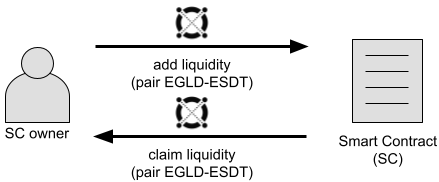
\includegraphics[width=\linewidth]{cu_add_claim_liquidity.png}
  \caption{Requerimens funcionals 1 i 2.}\label{fig:addclaimliq}
\end{subfigure}\hfill
\begin{subfigure}[b]{0.49\textwidth}
  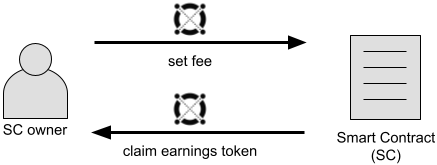
\includegraphics[width=\linewidth]{cu_set_fee_claim_earnings.png}
  \caption{Requisits funcionals 3 i 4.}\label{fig:setfeeclaim}
\end{subfigure}\hfill
\caption{Interaccions del propietari amb el contracte intel·ligent.}
\end{figure}

Amb les interaccions anteriors es podran \textbf{definir \textit{liquity pools}} i una \textbf{taxa (\textit{fee})} que es cobrarà per les operacions de \textit{swap}. El següent a definir seran els intercanvis en si mateixos. El criptoactiu de referència serà xEGLD (tots els parells el tindran). Així es podrà passar una determinada quantitat d'un token ESDT a xEGLD. Això també es pot anomenar ``\textbf{comprar ESDT amb EGLD}''. A la inversa, podrem passar xEGLD a ESDT, que dit d'altra forma seria ``\textbf{vendre ESDT per EGLD}''. La següent figura ho mostra:
\begin{figure}[h]
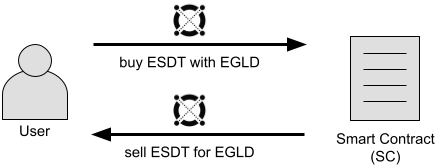
\includegraphics[width=0.5\textwidth]{cu_buy_sell1.png}
\centering
\caption{RF 5. Operacions de compra i venda de \textit{tokens} (\textit{swaps}).}\label{fig:cu_buy_sell1}
\end{figure} 

Per altra banda, serà necessari que el sistema mostri als usuaris els \textbf{parells disponibles per fer intercanvis i si es pot operar amb ells en un moment donat} (requisits funcionals 6 i 7).

\begin{figure}[!htb]
\begin{subfigure}[b]{0.49\textwidth}
  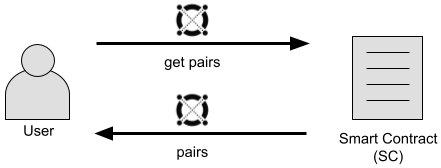
\includegraphics[width=\linewidth]{cu_get_pairs.png}
  \caption{RF 6.}\label{fig:getpairs}
\end{subfigure}\hfill
\begin{subfigure}[b]{0.49\textwidth}
  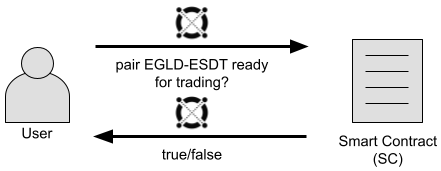
\includegraphics[width=\linewidth]{cu_status_pair.png}
  \caption{RF 7.}\label{fig:statuspair}
\end{subfigure}\hfill
\caption{Parells donats d'alta preparats per a intercanvis.}
\end{figure}

A més, el sistema mostrarà la \textbf{constant \(k\) del protocol AMM} (que s'ha de mantenir constant) i el \textbf{preu dels actius en el moment actual}. Internament es treballa amb nombres enters on es destinen les 18 posicions a la dreta per a decimals, però realment són nombres enters. Això farà que la constant \(k\) pugui fluctuar i que estigui sotmesa a correccions per mantenir-la en el seu valor inicial. Així mateix, els usuaris hauran de conèixer en temps real els preus de les parelles de tokens. Els casos d'ús sobre aquests punts es mostren en la Fig. \ref{fig:RRFF8-9}.

\begin{figure}[!htb]
\begin{subfigure}[b]{0.33\textwidth}
  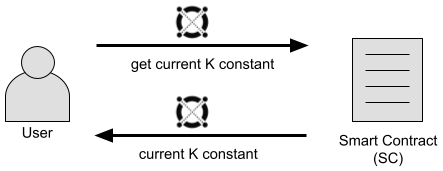
\includegraphics[width=\linewidth]{cu_k_constant.png}
  \caption{RF 8.}\label{fig:kconstant}
\end{subfigure}\hfill
\begin{subfigure}[b]{0.33\textwidth}
  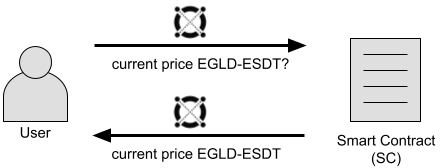
\includegraphics[width=\linewidth]{cu_current_price_EGLD_ESDT.png}
  \caption{RF 9 (EGLD-ESDT).}\label{fig:price_egld_esdt}
\end{subfigure}\hfill
\begin{subfigure}[b]{0.33\textwidth}
  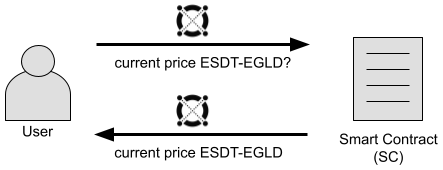
\includegraphics[width=\linewidth]{cu_current_price_ESDT_EGLD.png}
  \caption{RF 9 (ESDT-EGLD).}\label{fig:price_esdt_egld}
\end{subfigure}\hfill
\caption{Valor actual de la constant \(k\) i preus de compra-venda dels parells de \textit{tokens}.}
\label{fig:RRFF8-9}
\end{figure}

\begin{figure}[h]
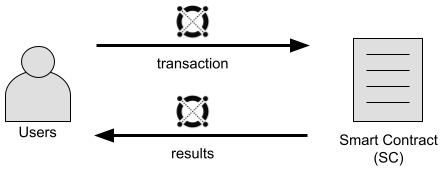
\includegraphics[width=0.55\textwidth]{cu_trans_results.png}
\centering
\caption{Requisit funcional 10.}\label{fig:transresults}
\end{figure} 

Finalment, pel que fa al RF 10 i als \textbf{requisits no funcionals}, no cal afegir res ja que formen part de les característiques intrínseques de les tecnologies d'Internet i de la xarxa Elrond.

\subsubsection{\textit{Smart contract}}\label{subsub:sc}
Totes les dades dels \textit{smart contracts} de la xarxa Elrond són disponibles públicament, tot i que pot ser complicat cercar manualment l'emmagatzematge del contracte i per això es solen definir \textit{getters} públics\footnote{Quan s'implementin les propietats i mètodes públics en el lleguatge Rust s'anotaran amb \#[endpoint] o \#[view].}. Quan es desplegui a la xarxa se li assignarà automàticament una adreça amb el format que s'ha descrit en seccions anteriors.

En la Fig. \ref{fig:testdex} es mostren les propietats i mètodes del contracte intel·ligent que emprarem (anomenat ``TestDEX''). Cal dir, que en argot específic de \textit{blockchain} seria més apropiat anomenar a una propietat ``emmagatzematge''. 

\begin{figure}[h]
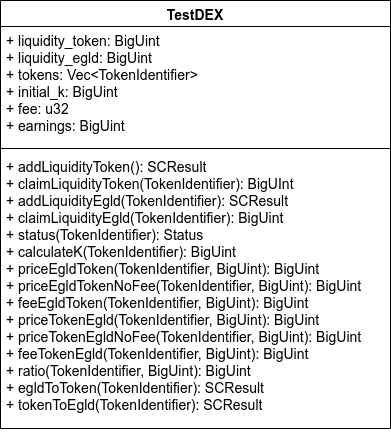
\includegraphics[width=0.55\textwidth]{TestDEX.png}
\centering
\caption{Estructura del contracte intel·ligent.}\label{fig:testdex}
\end{figure} 

La descripció dels ``emmagatzematges'' és la següent:
\begin{itemize}
\item \textbf{liquidity\_token(TokenIdentifier)}: Emmagatzema la liquiditat dels \textit{tokens} (la meitat del parell). Per als identificadors del token de què vulguem guardar la informació, tindrem un valor del tipus BigUint\footnote{Estructura de dades que representa un nombre enter molt gran sense signe.} associat que definirà la seva quantitat acumulada en el contracte intel·ligent. Disposa d'un \textit{getter} \textbf{getLiquidityToken} (amb el mateix paràmetre).
\item \textbf{liquidity\_egld(TokenIdentifier)}: Guarda la liquiditat en EGLD dels \textit{tokens} (l'altra part del parell). Per als identificadors dels tokens dels que vulguem guardar la informació, tindrem un valor del tipus BigUint associat que definirà la quantitat d'EGLD. Disposa d'un \textit{getter} \textbf{getLiquidityEgld} (amb el mateix paràmetre).
\item \textbf{initial\_k(TokenIdentifier)}: Per a cada parell \textit{token}-EGLD emmagatzema un BigUint amb la seva constant \(k\) del moment en què es va donar d'alta.  Disposa d'un \textit{getter} \textbf{getInitialK} (amb el mateix paràmetre).
\item \textbf{fee}: Guarda la taxa –amb un valor del tipus u32\footnote{Sencer sense signe representat amb 32 bits.}– que s'aplicarà quan es faci un intercanvi. S'inicialitza quan es creï el contracte intel·ligent. Disposa d'un \textit{getter} \textbf{getFee}.
\item \textbf{earnings\_egld(TokenIdentifier)}: Emmagatzema les taxes (\textit{fees}) –BigUint– cobrades pels diferents \textit{tokens}. Disposa d'un \textit{getter} \textbf{getEarnings} (amb el mateix paràmetre).
\end{itemize}
Pel que fa als mètodes:
\begin{itemize}
\item \textbf{init(u32)}: Mètode que realitza la tasca de constructor del contracte intel·ligent. Se li passa la taxa que es cobrarà en els intercanvis.
\item \textbf{addLiquidityToken() -\textgreater SCResult}: Afegeix liquiditat a la part ``\textit{token}'' del parell. Retorna un valor del tipus SCResult, forma predeterminada de retornar opcionalment un error (\(Err(SCError)\)) o una confirmació de resultat satisfactori (\(Ok(T)\)). El token i la quantitat les agafarà de la mateixa transacció dins de la xarxa Elrond. Mètode que només pot ser cridat pel propietari del contracte.
\item \textbf{claimLiquidityToken(TokenIdentifier)  -\textgreater SCResult}: Envia els fons de liquiditat d'un \textit{token} determinat aportats pel propietari del contracte intel·ligent a l'adreça del seu moneder. Se li ha de passar com a paràmetre l'identificador del \textit{token} de què volem reclamar la liquiditat. Mètode que només pot ser cridat pel propietari del contracte. Retorna un BigUint equivalent a la quantitat transferida. Només es torna la part ``token''. El parell quedarà en estat ``Funding''.
\item \textbf{addLiquidityEgld(TokenIdentifier)  -\textgreater SCResult}: Afegeix liquiditat a la part EGLD del parell. Se li ha de passar com a paràmetre l'identificador d'EGLD. La quantitat l'agafarà de la mateixa transacció dins de la xarxa Elrond. Mètode que només pot ser cridat pel propietari del contracte.
\item \textbf{claimLiquidityEgld(TokenIdentifier)  -\textgreater SCResult}: Envia els fons de liquiditat en EGLD del parell d'un determinat \textit{token} aportats pel propietari del contracte intel·ligent a l'adreça del seu moneder. Se li ha de passar com a paràmetre l'identificador del \textit{token} de què volem guardar la informació. Mètode que només pot ser cridat pel propietari del contracte. Retorna un BigUint equivalent a la quantitat transferida. El parell quedarà en estat ``Funding''.
\item \textbf{status(TokenIdentifier) -\textgreater Status}: Mostra l'estat d'un parell. Tindrà dos possibles estats: ``Successful'' i ``Funding''. El primer significa que està preparat per fer intercanvis i el segon indica que encara s'han d'afegir fons a algun dels components del parell. Se li ha de passar com a paràmetre l'identificador del \textit{token} de què volem retornar aquesta informació. Retorna o bé ``Successful'' o bé ``Funding''.
\item \textbf{calculateK(TokenIdentifier) -\textgreater BigUint}: Calcula la constant \(k\) per a un parell en un moment donat de temps. Se li ha de passar com a paràmetre l'identificador del \textit{token} que identifica el parell de què volem retornar aquesta informació (el que no sigui EGLD). Retorna la citada constant.
\item \textbf{claimEarnings(TokenIdentifier) -\textgreater BigUint}: Envia els beneficis acumulats resultants d'aplicar la taxa als intercanvis d'un \textit{token} determinat al contracte. Se li ha de passar com a paràmetre l'identificador del \textit{token} de què volem transferir els beneficis. Mètode que només pot ser cridat pel propietari del contracte. Retorna un BigUint equivalent a la quantitat transferida.
\item \textbf{priceEgldToken(TokenIdentifier, BigUint) -\textgreater BigUint}: Calcula el preu d'una certa quantitat d'un \textit{token} determinat en EGLD aplicant la taxa (\textit{fee}). Se li ha de passar com a arguments l'identificador del \textit{token} de què volen calcular el preu i la citada quantitat. Retorna el preu com a nombre enter.
\item \textbf{priceEgldTokenNoFee(TokenIdentifier, BigUint)-\textgreater BigUint}: És igual que l'anterior però al preu retornat no se li aplica la taxa.
\item \textbf{feeEgldToken(TokenIdentifier, BigUint) -\textgreater BigUint}:  Calcula la taxa que es pagarà per una certa quantitat d'un \textit{token} en EGLD. Se li han de passar com a arguments l'identificador del \textit{token} de què volen calcular el preu i la citada quantitat. Retorna aquest cost com a nombre enter.
\item \textbf{priceTokenEgld(TokenIdentifier, BigUint) -\textgreater BigUint}: Calcula el preu d'una certa quantitat d'EGLD en un \textit{token} determinat. Se li han de passar com a arguments l'identificador del \textit{token} amb què volem pagar i la quantitat d'EGLD que volem obtenir. Retorna el preu com a nombre enter. S'aplica la taxa (\textit{fee}).
\item \textbf{priceTokenEgldNoFee(TokenIdentifier, BigUint) -\textgreater BigUint}: Igual que l'anterior però al preu retornat no se li aplica la taxa.
\item \textbf{feeTokenEgld(TokenIdentifier, BigUint) -\textgreater BigUint}: Calcula la taxa que es pagarà per una certa quantitat d'EGLD en un \textit{token} determinat. Se li han de passar com a arguments l'identificador del \textit{token} i la citada quantitat. Retorna aquest cost com a nombre enter.
\item \textbf{swapEgldForToken(TokenIdentifier) -\textgreater SCResult}: Per intercanviar \textit{tokens} per EGLD. La quantitat d'EGLD s'agafarà de la transacció. S'enviarà la quantitat del \textit{token} al moneder de l'usuari que faci la compra. Les taxes pagades s'acumularan al contracte intel·ligent. S'haurà de passar com a argument l'identificador del \textit{token} que es vol comprar. Les taxes es llevaran de la quantitat que ha de rebre l'usuari com a resultat de l'intercanvi.
\item \textbf{swapTokenForEgld(TokenIdentifier) -\textgreater SCResult}: El sentit invers de l'anterior, comprar EGLD amb \textit{token}. El \textit{token} i la quantitat d'EGLD s'agafaran de la transacció. S'enviarà la quantitat d'EGLD al moneder de l'usuari que faci la compra. Les taxes pagades s'acumularan al contracte intel·ligent (es llevaran de la quantitat que ha de rebre l'usuari com a resultat de l'intercanvi).
\end{itemize}
 
Com ja s'ha dit, Elrond VM es basa en WebAssembly (WASM). A l'especificació \textbf{se li ha llevat el suport a les operacions de coma flotant} \cite{mincub2020}. Això ha provocat que s'hagin d'haver adaptat les fórmules desenvolupades en la secció \ref{subsub:dexamm}. D'aquesta forma, per a certs mètodes del contracte intel·ligent en generaran dos de nous: un mètode que retorni el numerador i un altre que retorni el denominador. La idea de fer aquesta separació és fer les operacions de divisió a la DApp (que sí que permet operar amb decimals). Això té certa importància a nivell visual per a l'usuari, ja que és més comprensible llegir ``1.21 xEGLD'' que no pas ``1210000000000000000 wei''. A part d'això, es generava també el problema de què la taxa (\textit{fee}) no podia ser un nombre decimal. Això ha implicat que, a part de separar en numerador i denominador, es transformin les citades equacions de la següent forma perquè aquesta comissió sigui un nombre enter:\footnote{Idea extreta dels exercicis que desenvolupen el material didàctic descrit a \cite{delarosa}.}
\[t'_x = \frac{x * t_y *(1000 - fee)}{1000 * y + t_y * (1000 - fee)}\]
\[t'_{x_{numerador}} = x * t_y *(1000 - fee)\]
\[t'_{x_{denominador}} = 1000 * y + t_y * (1000 - fee)\]
\[t'_y = \frac{y * t_x * (1000 - fee)}{1000 * x + t_x * (1000 - fee)} \]
\[t'_{y_{numerador}} = y * t_x * (1000 - fee)\]
\[t'_{y_{denominador}} = 1000 * x + t_x * (1000 - fee)\]
Amb aquests canvis, \textit{fee} podrà ser un nombre enter. Com ja hem vist, un valor de 5 aplicarà una taxa del 0,5\%.

En resum, per separar el numerador i el denominador i aplicant el citat canvi perquè la taxa sigui un nombre enter, s'han hagut d'afegir al contracte intel·ligent:
\begin{itemize}
\item Pel mètode priceEgldTokenNumerator apareixen els nous:
	\begin{itemize}
		\item priceEgldTokenNumerator
		\item priceEgldTokenDenominator
	\end{itemize}
\item Pel mètode priceEgldTokenNoFee apareixen els nous:
	\begin{itemize}
		\item priceEgldTokenNoFeeNumerator
		\item priceEgldTokenNoFeeDenominator
	\end{itemize}	
\item Pel mètode priceTokenEgld apareixen els nous:
	\begin{itemize}
		\item priceTokenEgldNumerator
		\item priceTokenEgldDenominator
	\end{itemize}
\item I, finalment, del mètode priceTokenEgldNoFee apareixen els nous:
	\begin{itemize}
		\item priceTokenEgldNoFeeNumerator
		\item priceTokenEgldNoFeeDenominator
	\end{itemize}		
\end{itemize}

\subsubsection{Arquitectura}\label{subsub:arq}

Una \textbf{DApp} ens permetrà escriure en la blockchain i llegir l'emmagatzematge –o estat– del contracte intel·ligent descrit en l'apartat anterior. Com es pot comprovar en la Fig. \ref{fig:architecture}, \textbf{per escriure en la cadena de blocs} la DApp haurà de llençar una \textbf{transacció} que invoqui a un mètode del contracte. Si per contra només necessitem \textbf{llegir l'estat} del contracte intel·ligent, emprarem una \textbf{API} aportada per Elrond per invocar certs mètodes del contracte, cosa que no farà pas cap canvi en la cadena de blocs.

\begin{figure}[h]
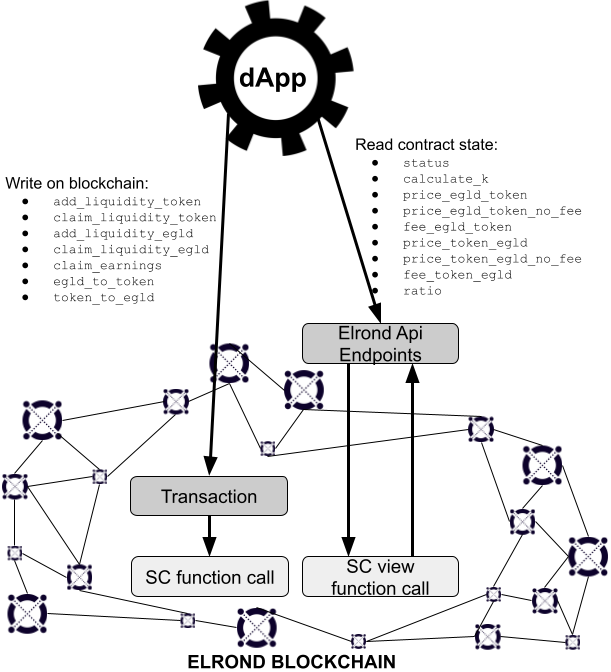
\includegraphics[width=0.75\textwidth]{architecture.png}
\centering
\caption{Arquitectura de testDEX. (Font: Elaboració pròpia inspirada en \cite{elrond2022}).}\label{fig:architecture}
\end{figure} 

Pot parèixer una descripció molt breu, però és que és veritablement una arquitectura molt senzilla.

\subsubsection{Pantalles}

Per \textbf{accedir a la DApp} s'haurà de triar un dels mètodes habilitats per fer-ho a la xarxa Elrond (Fig. \ref{fig:screenlogin}).

\begin{figure}[!htb]
\begin{subfigure}[b]{0.39\textwidth}
  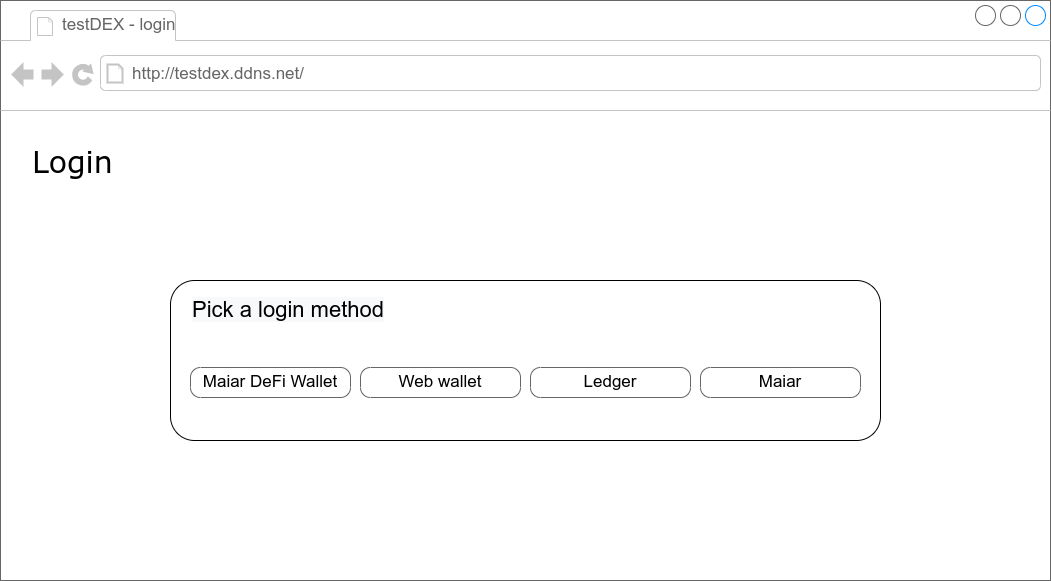
\includegraphics[width=\linewidth]{screen_login.png}
  \caption{Finestra de login.}\label{fig:screenlogin}
\end{subfigure}\hfill
\begin{subfigure}[b]{0.59\textwidth}
  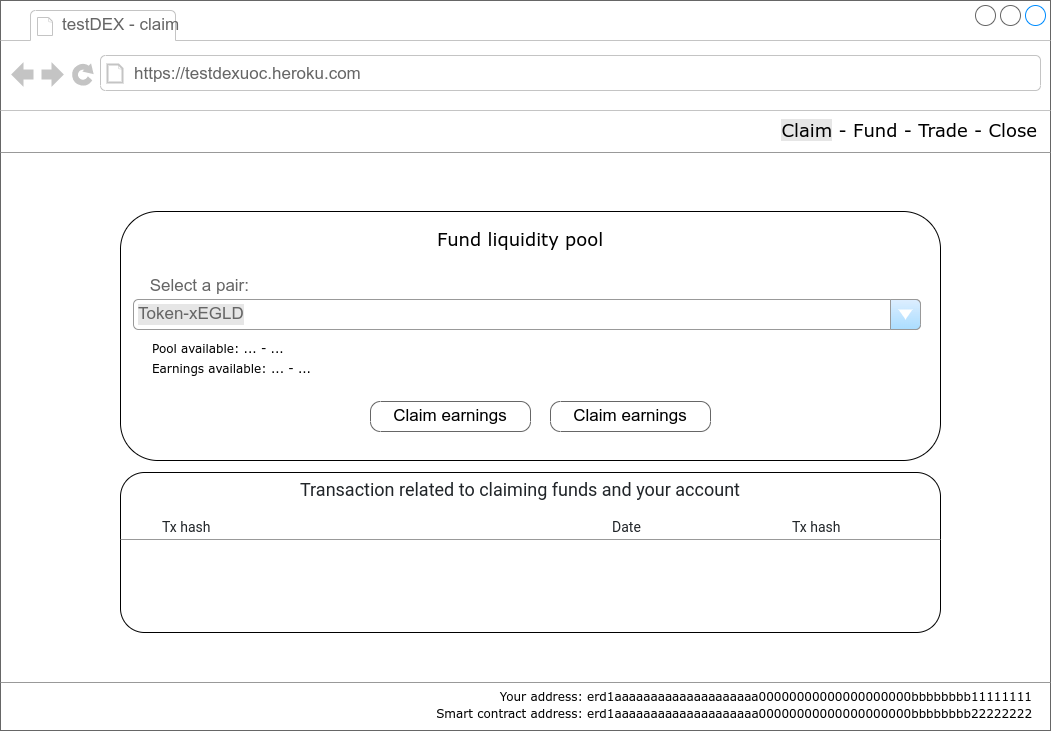
\includegraphics[width=\linewidth]{screen_claim.png}
  \caption{Finestra on reclamar els fons i els beneficis.}\label{fig:screenclaim}
\end{subfigure}\hfill
\caption{Finestres ``Login'' i ``Claim''.}
\end{figure}

Només per a l'\textbf{usuari que sigui el propietari del contracte}, li apareixerà en el menú d'adalt a la dreta les \textbf{opcions ``Claim'' i ``Fund''}. En la pantalla ``Fund'' es podran \textbf{crear els diferents fons de liquiditat del contracte intel·ligent} (Fig. \ref{fig:screenfund}) i en la finestra ``Claim'' es podran reclamar els fons i els beneficis obtinguts (Fig. \ref{fig:screenclaim}). S'ha de destacar que els fons una vegada creats, ja no es poden modificar a no ser que es realitzin \textit{swaps} en la finestra de ``Trade''. També es poden reclamar a la finestra ``Claim'' i a partir d'aquí es poden tonar a crear.

\begin{figure}[!htb]
\begin{subfigure}[b]{0.47\textwidth}
  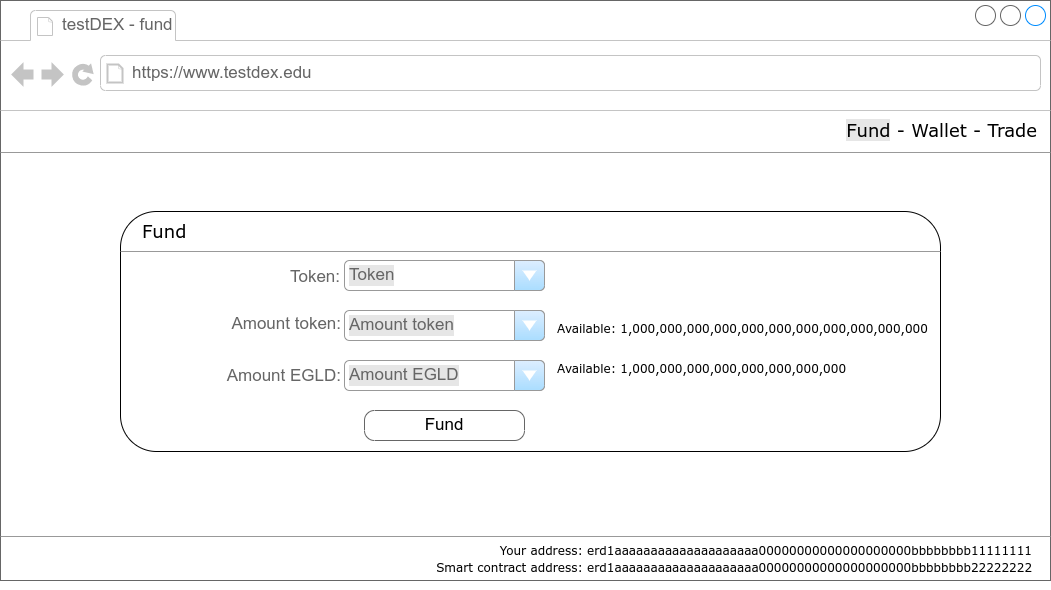
\includegraphics[width=\linewidth]{screen_fund.png}
  \caption{Finestra on s'aprovisionen els \textit{liquidity pools}.}\label{fig:screenfund}
\end{subfigure}\hfill
\begin{subfigure}[b]{0.47\textwidth}
  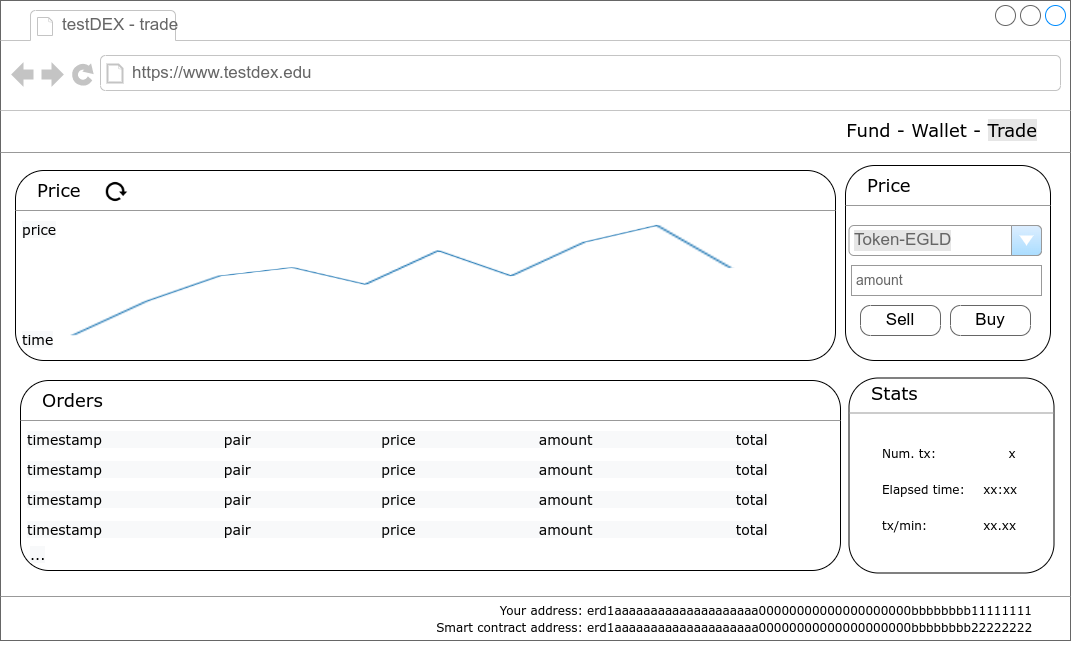
\includegraphics[width=\linewidth]{screen_trade.png}
  \caption{Finestra on es poden realitzar els \textit{swaps}.}\label{fig:screentrade}
\end{subfigure}\hfill
\caption{Finestres ``Fund'' i ``Trade''.}
\end{figure}

En l'\textbf{opció del menú ``Trade''} trobem la finestra amb el cor de l'aplicació (Fig. \ref{fig:screentrade}). Es podran \textbf{seleccionar els parells dels quals s'han donat d'alta fons de liquiditat i realitzar compres o vendes}. Es mostraran les dades referents a les operacions que es faran (quantitat de \textit{tokens} que rebrem si els comprem amb xEGLD prement el botó ``\textit{Buy}'' o quantitat de xEGLD que rebrem si venem el citat \textit{token} prement el botó ``\textit{Sell}''). També apareixeran les quantitats disponibles del parell dins del \textit{pool} i dins de la \textit{wallet} de l'usuari. Abaix a la dreta es pot observar que es veurà l'estat de la constant \(k\) en el moment actual (``\textit{Current k}'') i quan es va inicialitzar el fons (``\textit{Initial k}'')

\subsection{Implementació}\label{sec:imp}
\subsubsection{Repositoris disponibles}
He dividit el projecte en quatre repositoris a Github:
\begin{itemize}
\item \textbf{TFM\_latex}\footnote{\url{https://github.com/sergiogrubio/TFM_latex}}: El present document amb tots els recursos necessaris per generar-lo.
\item \textbf{TFM\_smart\_contract}\footnote{\url{https://github.com/sergiogrubio/TFM_smart_contract}}: Contracte intel·ligent del projecte escrit en Rust (es pot consultar en l'arxiu ``testdex.rs''). Es troben també altres recursos necessaris per compilar-lo, així com d'altres per fer-ne proves.
\item \textbf{TFM\_DApp}\footnote{\url{https://github.com/sergiogrubio/TFM_DApp}}: Aquí es troba la DApp que interacciona amb el contracte intel·ligent del punt anterior. Es basa en la plantilla ``DApp-template'' aportada per Elrond\footnote{\url{https://github.com/ElrondNetwork/DApp-template}}.
\item \textbf{TFM\_stats}\footnote{\url{https://github.com/sergiogrubio/TFM_stats}}: Es tracta d'un \textit{script} escrit en Python per comprovar el rendiment de la xarxa d'Elrond. Es llançaran peticions emprant \textit{erdpy} al contracte intel·ligent descrit.  
\end{itemize}

\subsubsection{Aspectes a destacar de la implementació}\label{imp:aspectes}
En primer lloc, vull destacar les diferents formes en què s'ha interactuat des de la DApp amb la \textit{blockchain}:
\begin{itemize}
\item \textbf{Transferències ESDT}: Són transaccions signades. Tenen la característica de què el valor de la transacció (camp ``\(value\)'') serà de 0 xEGLD. El token, la quantitat del mateix, el mètode que es trucarà del \textit{smart contract} i els respectius paràmetres aniran dins del camp ``\(data\)'' (al principi d'aquest camp s'indicarà que és aquest tipus de transferència amb el text ``\(ESDTTransfer\)''). Es pot observar en la Fig. \ref{fig:impesdttransfer}.
\item \textbf{Transferències de xEGLD}: També són transaccions signades. En el camp ``\(value\)'' anirà el valor de la transacció expressat en ``wei'' d'EGLD. En el camp ``\(data\)'' es posarà el mètode que es trucarà del \textit{smart contract} i els respectius paràmetres.
\item \textbf{\textit{Queries} al smart \textit{contract}}: No duen associada una transacció signada. Es demana l'execució d'un mètode del contracte intel·ligent que no duu associat cap transferència d'actius, simplement consulta l'estat d'aquest. En la Fig. \ref{fig:imp-queryapirest} es pot observar un exemple.
\item \textbf{Consulta a l'API REST de la devnet d'Elrond}\footnote{\url{https://devnet-api.elrond.com/}}: S'ha comentat de passada la seva existència a la secció \ref{sub:altres}. Permet consultar dades sobre l'estat dels diferents elements de la devnet d'Elrond (òbviament, existeixen les respectives versions per a les altres xarxes). La seva utilitat m'ha semblat determinant. Per exemple, l'empro per consultar els actius del moneder d'un client o els actius disponibles en el contracte intel·ligent. Un exemple d'ús es pot consultar en la Fig. \ref{fig:imp-queryapirest}. 
\end{itemize}

\begin{figure}[!htb]
\begin{subfigure}[b]{0.47\textwidth}
  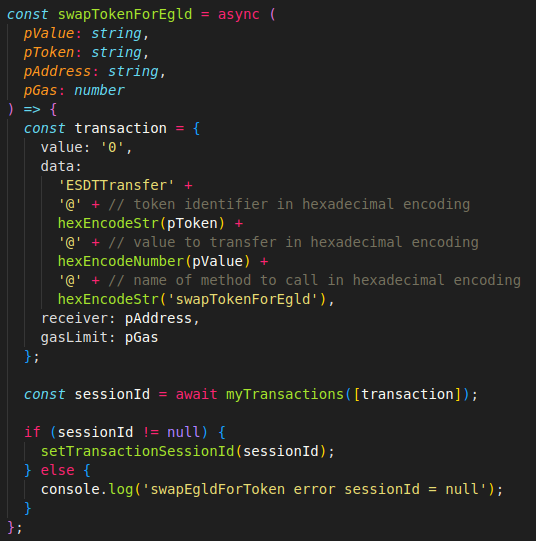
\includegraphics[width=\linewidth]{imp-esdttransfer.png}
  \caption{Exemple de transferència ESDT.}\label{fig:impesdttransfer}
\end{subfigure}\hfill
\begin{subfigure}[b]{0.47\textwidth}
  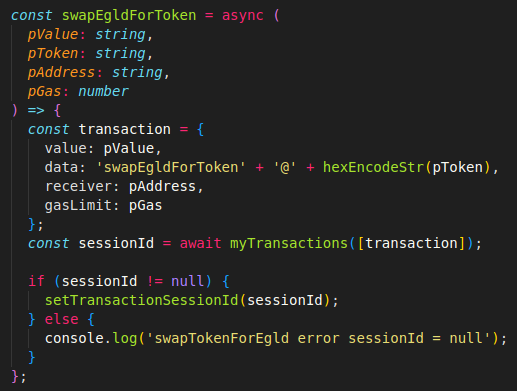
\includegraphics[width=\linewidth]{imp-egldtransfer.png}
  \caption{Exemple de transferència xEGLD.}\label{fig:screentrade}
\end{subfigure}\hfill
\caption{Els dos tipus de transferències d'actius en el codi font de la DApp.}
\label{fig:tipustransfer}
\end{figure}

\begin{figure}[h]
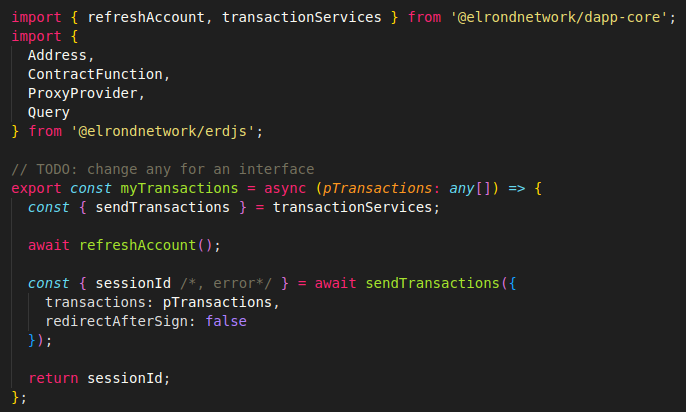
\includegraphics[width=0.65\textwidth]{imp-mytransactions.png}
\centering
\caption{Funció emprada en les transferències de la Fig. \ref{fig:tipustransfer}.}
\end{figure} 

\begin{figure}[h]
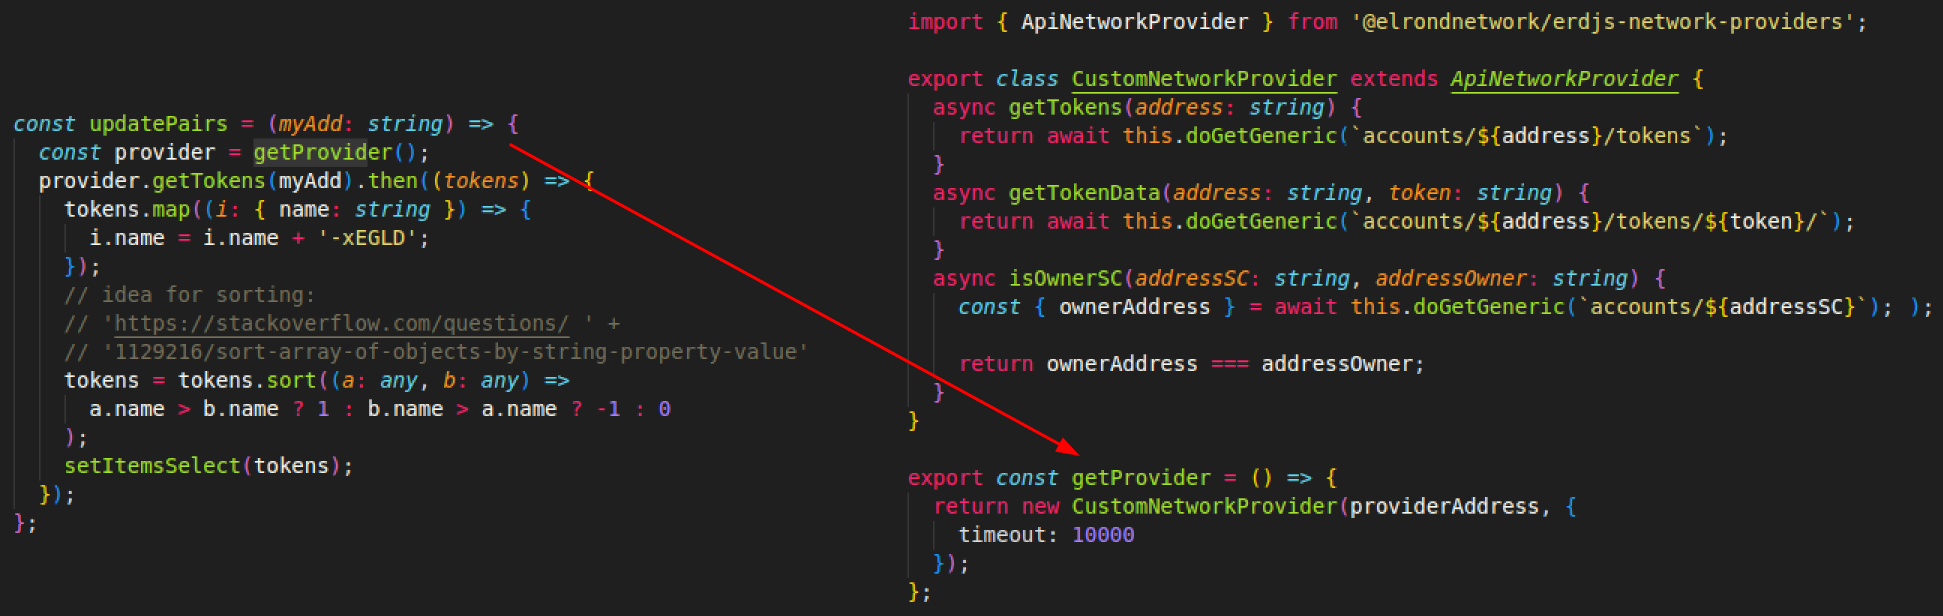
\includegraphics[width=0.65\textwidth]{imp-queryapirest.png}
\centering
\caption{Consultes a l'API REST de la devnet d'Elrond.}\label{fig:imp-queryapirest}
\end{figure} 

\subsubsection{\textit{Correcció de la constant \(k\) per l'error introduït per l'arrodoniment}}
Com s'ha comentat en la part de disseny, a la màquina virtual d'Elrond se li ha llevat el suport a les operacions de coma flotant. Com s'ha dit també, això provocarà que es vagi acumulant un error en la constant \(k\) que podria desvirtuar la natura del protocol AMM. Així com està implementat el \textit{smart contract}, aquest error es va acumulant en el fons del contracte intel·ligent. Òbviament, és un error lleu que farà que el propietari del \textit{pool} tingui més benefici. Mostra d'aquest error que es va acumulant es pot veure en la Fig. \ref{fig:imperrork}. Animo al lector que revisi la referència bibliogràfica \cite{zhang2018}.

\begin{figure}[h]
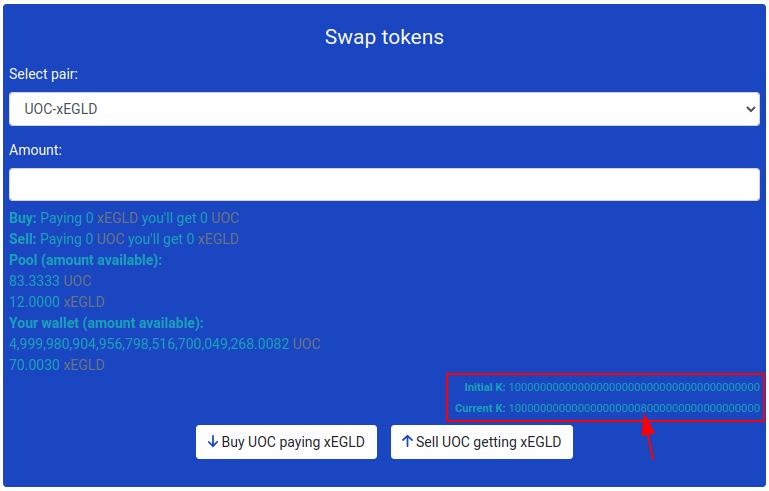
\includegraphics[width=0.75\textwidth]{imp-errork.png}
\centering
\caption{Error acumulat en la constant \(k\).}\label{fig:imperrork}
\end{figure} 

He dedicat temps a intentar solucionar el problema i he arribat a diverses solucions on la \(k\) es va ajustant quan passa per sota o per sobre del valor original. El problema d'aquestes solucions és que no les he pogut demostrar matemàticament (cosa no apropiada per a un treball acadèmic). En la Fig. \ref{fig:impcorrectk} es pot veure comentat un exemple d'aquestes proves (n'hi ha més al repositori de Github corresponent).

\begin{figure}[!htb]
\begin{subfigure}[b]{0.47\textwidth}
  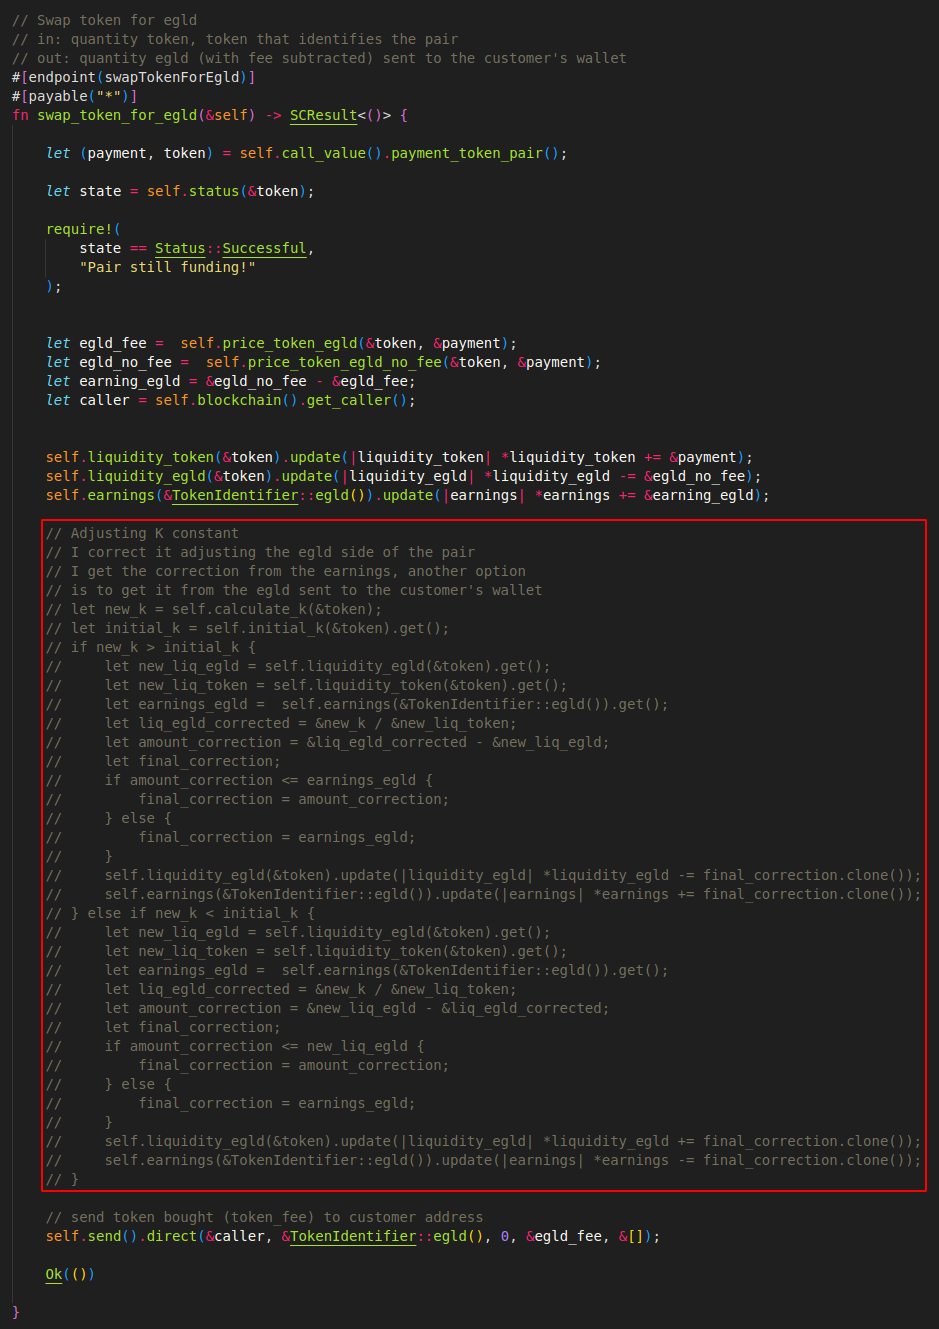
\includegraphics[width=\linewidth]{imp-sc01.png}
  \caption{Mètode ``swapTokenForEgld''.}\label{fig:impsc01}
\end{subfigure}\hfill
\begin{subfigure}[b]{0.47\textwidth}
  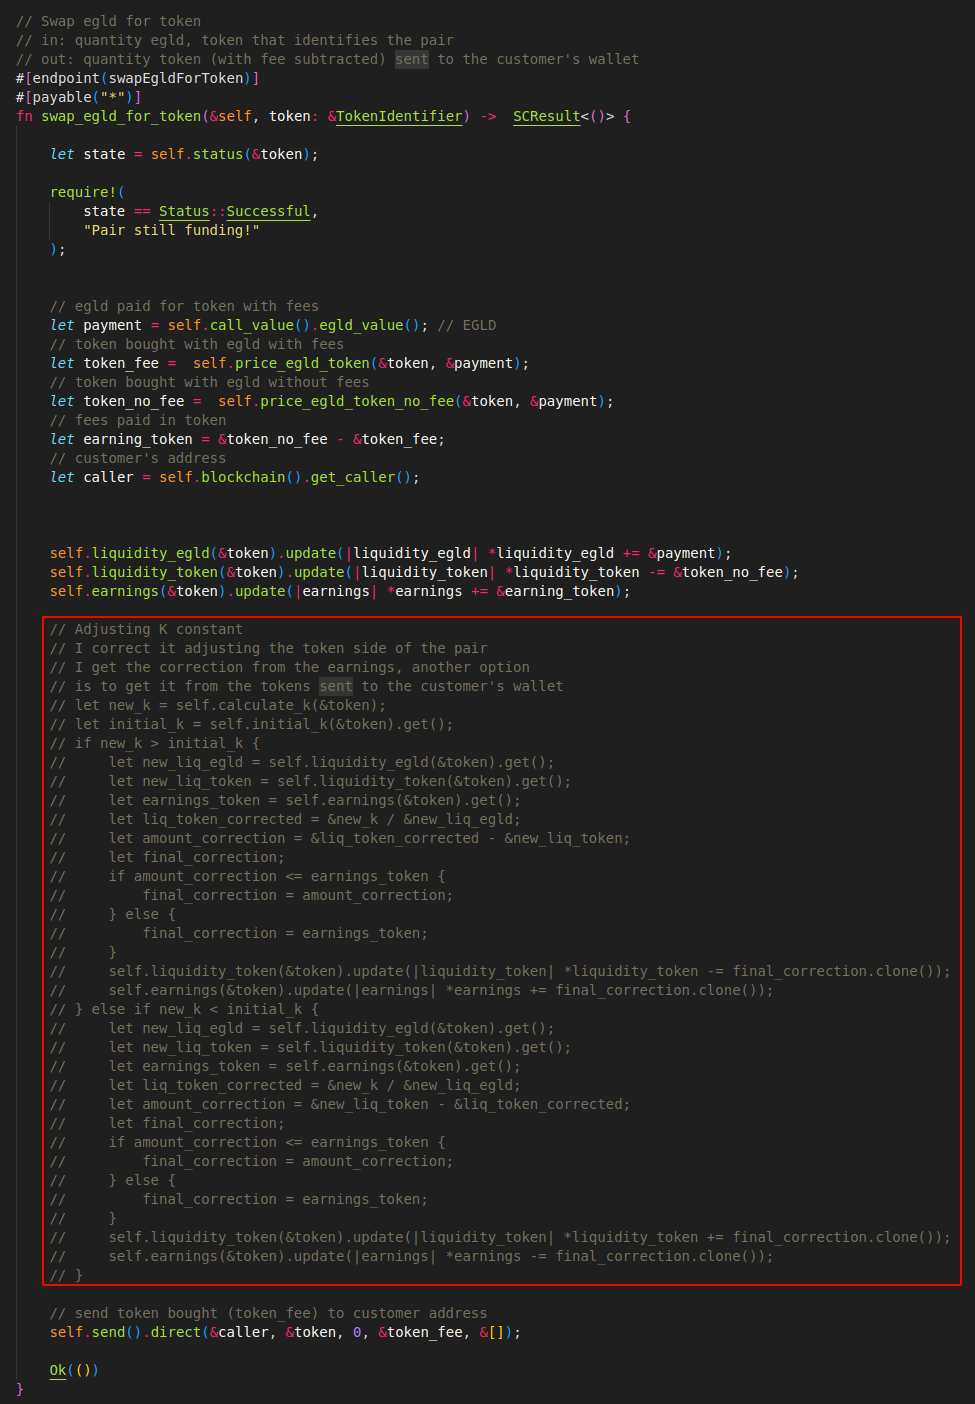
\includegraphics[width=\linewidth]{imp-sc02.png}
  \caption{Mètode ``swapEgldForToken''.}\label{fig:impsc02}
\end{subfigure}\hfill
\caption{Exemple d'implementació de l'ajustament de la constant \(k\).}
\label{fig:impcorrectk}
\end{figure}

\subsection{Posada en producció}
\subsubsection{Desplegament del contracte intel·ligent}
Començarem compilant el \textit{smart contract}. Executarem dins el directori on es trobi el codi font del contracte intel·ligent:\footnote{També es pot fer amb els \textit{snippets}, que seran explicats en la secció \ref{subsub:sc}.}.
\begin{lstlisting}[
    basicstyle=\footnotesize,
]
erdpy contract build
\end{lstlisting}

Amb això generarem el fitxer ``testdex.wasm'' que desplegarem a la \textit{devnet} d'Elrond amb la comanda:
\begin{lstlisting}[
    basicstyle=\footnotesize,
]
erdpy contract deploy --pem="~/wallet/wallet3.pem" \
  --recall-nonce --gas-limit=100000000 --project=. \
  --proxy="https://devnet-gateway.elrond.com" \
  --chain="D" --arguments 0x05 --send
\end{lstlisting}

D'entre els paràmetres, s'ha de destacar que dins de ``{\texttildelow/wallet/wallet3.pem}'' es troba la clau privada de l'usuari de la devnet d'Elrond que desplegarà el contracte intel·ligent a la xarxa (que serà el propietari) i amb ``-{}-arguments 0x05'' li passem en hexadecimal l'argument necessari per al mètode que fa de constructor (un valor de 5 implica una comissió del 0.5\%). Aquesta comanda mostrarà per la consola, entre altres coses, l'adreça del contracte intel·ligent dins de la \textit{devnet} d'Elrond. En el nostre cas:
\begin{lstlisting}[
    basicstyle=\footnotesize,
]
erd1qqqqqqqqqqqqqpgq578zh88hskf9efwzyhkf64el7d6ve3lrsn2qwkvmt2
\end{lstlisting}

\subsubsection{Desplegament de la DApp}
He donat d'alta dins del servei \url{noip.com} el nom testdex.ddns.net perquè apunti a un VPS (\textit{Virtual Private Server}) a OVH\footnote{\url{https://www.ovhcloud.com/}}. Al servidor he clonat el repositori amb l'ordre:
\begin{lstlisting}[
    basicstyle=\footnotesize,
]
git clone git@github.com:sergiogrubio/TFM_DApp.git
\end{lstlisting}
Dins del directori clonat he executat:
\begin{lstlisting}[
    basicstyle=\footnotesize,
]
npm run build
serve -s build
\end{lstlisting}
Després he fet una redirecció de ports amb:
\begin{lstlisting}[
    basicstyle=\footnotesize,
]
# localhost/loopback
sudo iptables -t nat -I OUTPUT -p tcp -d 127.0.0.1 --dport 80 \
	-j REDIRECT --to-ports 3000

# external
sudo iptables -t nat -I PREROUTING -p tcp --dport 80 -j REDIRECT \
	--to-ports 3000
\end{lstlisting}
La DApp estarà disponible durant el temps d'avaluació d'aquest TFM a l'URL:
\url{http://testdex.ddns.net/}. La única intenció és facilitar la revisió del treball (i no haver de clonar el repositori i executar-lo en local).

\subsection{Proves}
\subsubsection{Sobre el contracte intel·ligent}\label{subsub:sc}
Les proves sobre el contracte intel·ligent tenen una especial importància, ja que errades en el seu disseny i/o implementació poden provocar pèrdues econòmiques. Per testejar el contracte intel·ligent el primer que he fet és definir \textbf{``interaccions'' mitjançant \textit{snippets}} que empren l'eina \textit{erdpy}. En gerga d'Elrond, això seria ``crear un fitxer d'interaccions'' (en aquest cas anomenat ``devnet.snippets.sh''). Després fent clic amb el botó dret al \textit{plugin}\footnote{Com configurar l'entorn per desenvolupar en la xarxa Elrond es pot consultar en \cite{elrondnet2020} i \cite{ton2021}.} d'Elrond a Visual Studio Code podrem accedir als \textit{snippets} (Fig. \ref{fig:test-snippets}).

\begin{figure}[h]
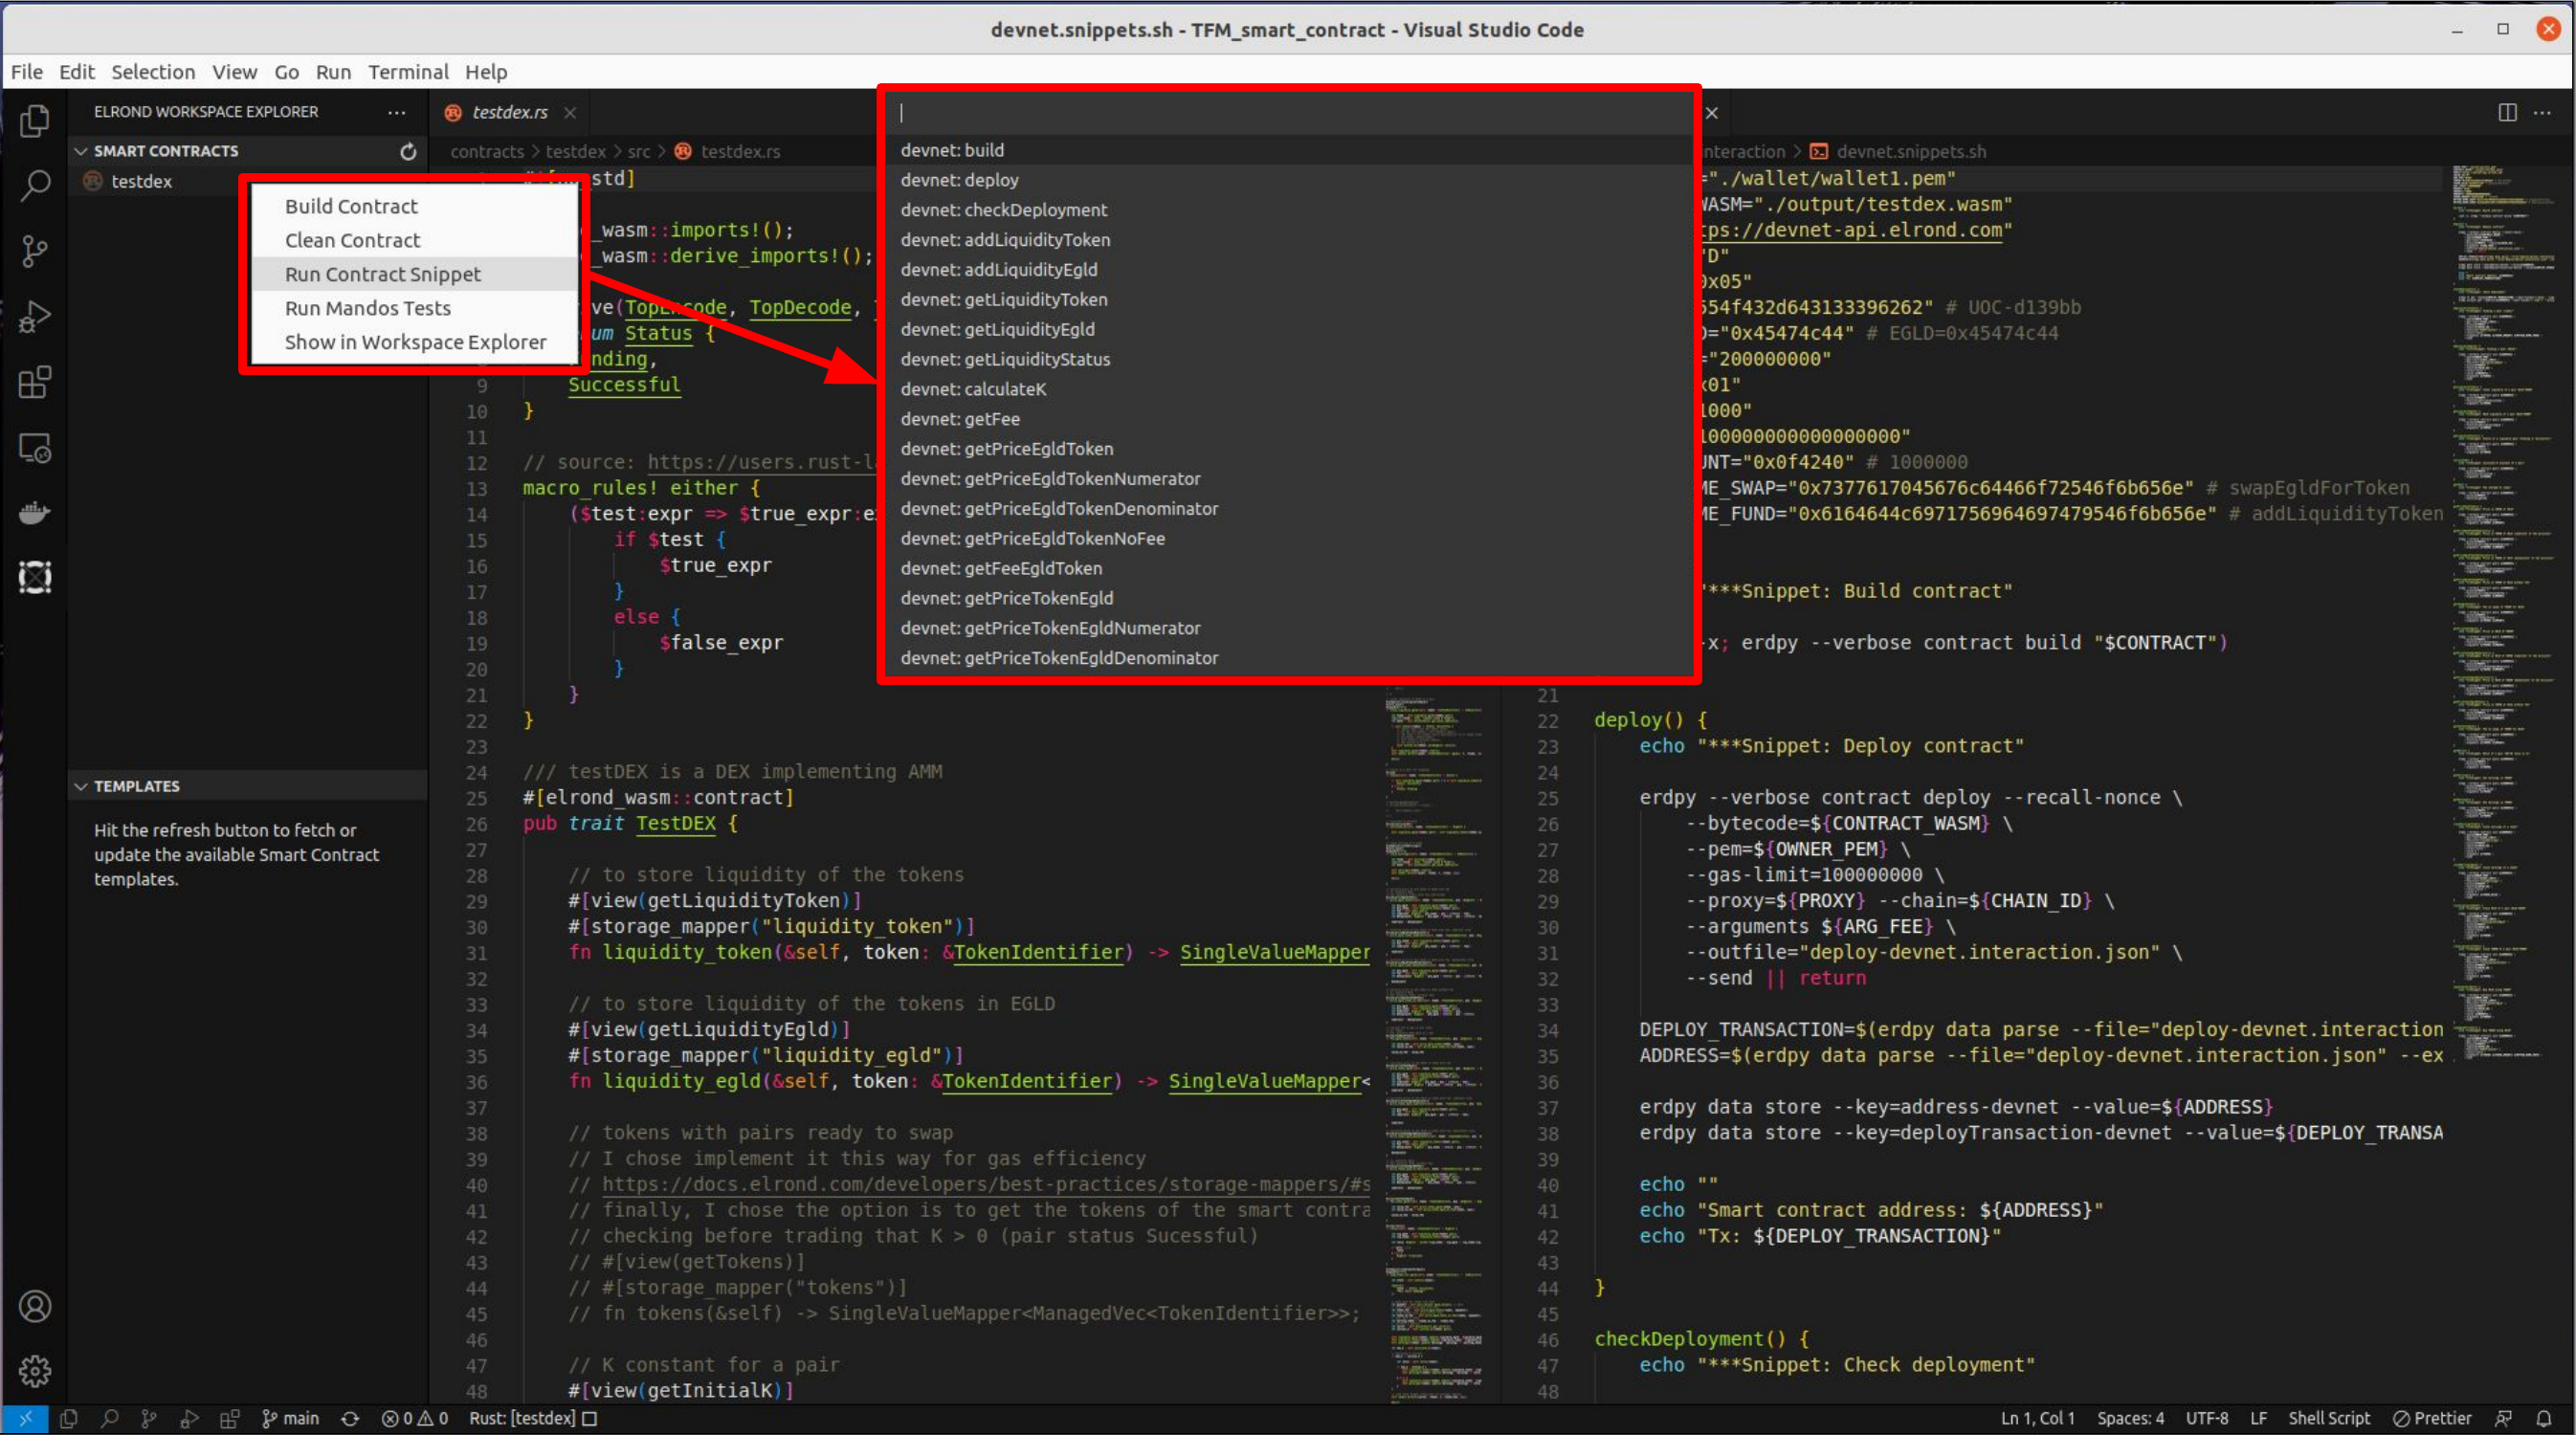
\includegraphics[width=1\textwidth]{test-snippets.png}
\centering
\caption{\textit{Snippets} en l'IDE Visual Studio Code.}\label{fig:test-snippets}
\end{figure} 

Hi ha definit un \textit{snippet} per a cada mètode del contracte intel·ligent, a més de dos addicionals per compilar-lo i desplegar-lo a la xarxa d'Elrond. Ja s'han comentat anteriorment els mètodes del contracte intel·ligent i els respectius \textit{snippets} permeten executar-los (i així comprovar si el comportament és l'esperat). Vull parar l'atenció en els que penso que són il·lustratius del funcionament d'\textit{erdpy}:
\begin{itemize}
\item \textbf{Trucades a mètodes del contracte intel·ligent que impliquen transferència d'actius} (\textit{erdpy contract call}):
	\begin{itemize}
	\item \textbf{Transferència d'EGLD del client cap al contracte} (\textit{snippet} ``addLiquidityEgld''): En la Fig. \ref{fig:test-addegld} es pot veure un exemple de com transferir EGLD al contracte intel·ligent. S'ha de destacar que l'opció ``-{}-value'' inclourà la quantitat d'EGLD a traspassar en wei i l'opció ``-{}-function'' especificarà el mètode del contracte amb la lògica que tractarà el citat moviment (els arguments que se li passen es definiran en ``-{}-arguments'' i estaran codificats en hexadecimal). Dins el mètode del contracte intel·ligent es podrà recuperar la quantitat d'EGLD amb:
\begin{lstlisting}
let payment = self.call\_value().egld\_value();
\end{lstlisting}
		\item \textbf{Transferència de tokens ESDT del client cap al contracte} (\textit{snippet} ``addLiquidityToken''): Aquest cas és un exemple de com transferir tokens ESDT (Fig. \ref{fig:test-addtoken}). Aquí no s'especificarà opció ``-{}-value'' i en l'opció ``-{}-function'' es posarà el text ``ESDTTransfer''. En l'opció arguments –codificat en hexadecimal– es passarà el nom del token, la quantitat del mateix i el nom del mètode del contracte amb la lògica per gestionar la trucada. Ja dins el mètode del contracte intel·ligent, el token i la quantitat es podran recuperar amb:
\begin{lstlisting}
let (payment, token) =
	self.call_value().payment_token_pair();
\end{lstlisting}
		\item \textbf{Transferència d'EGLD/token del contracte cap al client} (\textit{snippet} ``claimLiquidityToken''): Aquí es cridarà un mètode que generarà una transferència –tant d'EGLD com de tokens ESDT– cap a algun \textit{wallet} (Fig. \ref{fig:test-liquiditytoken}). L'opció ``-{}-value'' s'especificarà amb valor 0 i en l'opció ``-{}-function'' es posarà el mètode del contracte amb la lògica que tractarà el citat moviment (els arguments que se li passen es definiran en ``-{}-arguments'' i estaran codificats en hexadecimal).
	\end{itemize}
	\item \textbf{Trucades a mètodes del contracte intel·ligent sense transferència d'actius} (\textit{erdpy contract query}): En la Fig. \ref{fig:test-getearnings} es pot veure aquest cas. Serà suficient amb especificar el mètode que es crida i els arguments codificats en hexadecimal. Com que no es tracta d'una transacció que modifiqui la \textit{blokchain}, és molt més ràpida.
\end{itemize}

\begin{figure}[!htb]
	\begin{subfigure}[b]{0.40\textwidth}
	  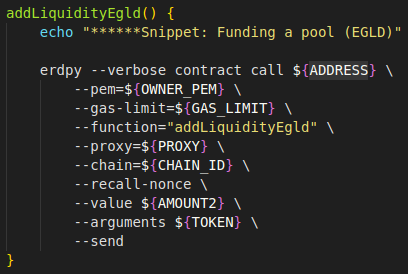
\includegraphics[width=\linewidth]{test-addegld.png}
	  \caption{``addLiquidityEgld''.}\label{fig:test-addegldsnip}
	\end{subfigure}\hfill
	\begin{subfigure}[b]{0.55\textwidth}
	  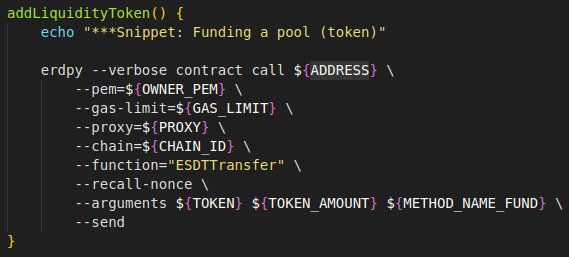
\includegraphics[width=\linewidth]{test-addtoken.png}
	  \caption{``addLiquidityToken''.}\label{fig:test-addtokensnip}
	\end{subfigure}\hfill
	\begin{subfigure}[b]{0.46\textwidth}
	  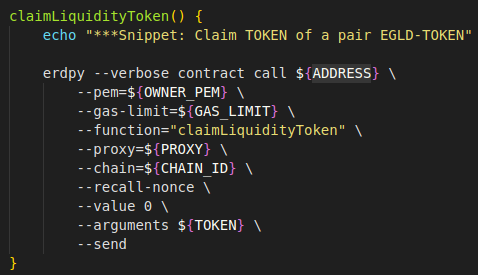
\includegraphics[width=\linewidth]{test-liquiditytoken.png}
	  \caption{``claimLiquidityToken''.}\label{fig:test-liquiditytoken}
	\end{subfigure}\hfill
	\begin{subfigure}[b]{0.39\textwidth}
	  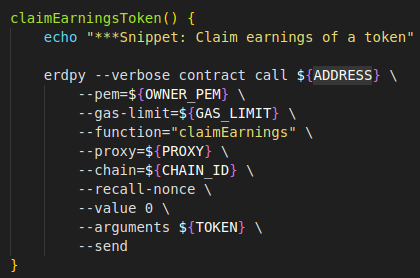
\includegraphics[width=\linewidth]{test-getearnings.png}
	  \caption{``claimEarningsToken''.}\label{fig:test-getearnings}
	\end{subfigure}\hfill
	\caption{\textit{Snippets} amb trucades a mètodes emprant \textit{erdpy}.}
\end{figure}

S'han executat els següents \textbf{\textit{snippets}} per validar el contracte intel·ligent\footnote{S'ha de destacar que en el resultat del \textit{snippet} apareixarà un enllaç cap a l'explorador de transaccions de la xarxa d'Elrond on es podrà comprovar si ha funcionat correctament o ha aparegut algun error (òbviament, es provaran situacions que haurien de generar error i en aquest cas el comportament anòmal és que funcioni correctament).}:

\begin{itemize}
\item \textbf{Compilar el contracte intel·ligent}: \textit{Snippet} ``build''.
\item \textbf{Desplegar el contracte intel·ligent}: \textit{Snippet} ``deploy''. Com a paràmetre si li passa la taxa (\textit{fee}) que es cobrarà en els \textit{swaps}.
\item \textbf{Comprovar que el contracte s'ha desplegat correctament}: \textit{Snippet} ``checkDeployment''.
\item \textbf{Afegir un fons de liquiditat}: \textit{Snippets} ``addLiquidityToken'' (Fig. \ref{fig:test-addegld}) i ``addLiquidityEgld'' (Fig. \ref{fig:test-addtoken}). Es torna a afegir fons al parell per comprovar que no deixa. Finalment, s'intenta crear un fons des d'una cartera que no és la propietaria del contracte intel·ligent per comprovar que dona error (dins del fitxer \textit{devenet.snippets.sh} s'ha de canviar la constant \textit{OWNER\_PEM=``./wallet/wallet1.pem''} per \textit{OWNER\_PEM=``./wallet/wallet2.pem''}).
\item \textbf{Obtenir la liquiditat del \textit{pool}}: \textit{Snippets} ``getLiquidityToken'' i ``getLiquidityEgld''. Òbviament, els valors obtinguts hauran de coincidir amb les quantitats que s'han d'especificar en la creació del fons en el punt anterior.
\item \textbf{Obtenir l'estat del fons de liquiditat}: \textit{Snippet} ``getLiquidityStatus''. Executat abans de constituir el fons i després de constituir-lo (ha de donar valors diferents).
\item \textbf{Calcular la constant K actual}: \textit{Snippets} ``calculateK'' i ``getRatio''. Per l'error de rendodeig en la divisió entre nombres enters que s'ha comentat abans, anirà fluctuant un poc per sobre i per sota del valor de la constant del moment de constituir el fons. S'ha comprovat fent \textit{swaps} que és així.
\item \textbf{Comprovar que la taxa (\textit{fee})}: \textit{Snippet} ``getFee''. La taxa ha de ser la mateixa que es va definir en el moment de desplegar el contracte intel·ligent. 
\item \textbf{Calcular el preu en token de l'EGLD (amb i sense taxa)}: \textit{Snippets} ``getPriceEgldToken'', ``getPriceEgldTokenNumerator'', ``getPriceEgldTokenDenominator'', ``getPriceEgldTokenNoFee'' i ``getFeeEgldToken''\footnote{\label{note1}Hi ha tres \textit{snippets} per coincidir amb la implementació que s'ha exposat en la secció \ref{subsub:sc}.}. S'ha comprovat que es generen els mateixos preus que en l'exemple descrit en la secció \ref{subsub:dexamm}.
\item \textbf{Calcular el preu en EGLD del token (amb i sense taxa)}: \textit{Snippets} ``getPriceTokenEgld'', ``getPriceTokenEgldNumerator'', ``getPriceTokenEgldDenominator'', ``getPriceTokenEgldNoFee'' i ``getFeeTokenEgld''\footnote{\ref{note1}}. S'ha comprovat que es generen els mateixos preus que en l'exemple descrit en la secció \ref{subsub:dexamm}.
\item \textbf{Comprovar els beneficis obtinguts pels swaps realitzats}: \textit{Snippets} ``getEarningsEgld'' i ``getEarningsToken''. També s'han comprovat que complien amb l'estudi teòric fet a la secció \ref{subsub:dexamm}.
\item \textbf{Comprovar que el propietari del contracte rep els beneficis d'un token concret quan els reclama}: \textit{Snippet} ``claimEarningsToken()''. S'ha d'emprar també el \textit{snippet} ``getEarningsToken'' per esbrinar la quantitat a rebre i després d'executar-lo ha d'aparèixer a la cartera del propietari del \textit{smart contract}.
\item  \textbf{Comprovar que el propietari del contracte rep els beneficis en EGLD quan els reclama}: {Snippet} ``claimEarningsEgld()''. S'ha d'emprar també el \textit{snippet} ``getEarningsEgld'' per esbrinar la quantitat a rebre i després d'executar-lo ha d'aparèixer a la cartera del propietari del \textit{smart contract}. Per disseny, l'EGLD que es recuperarà serà el generat amb tots els \textit{swaps} (independentment del parell).
\item  \textbf{Comprovar que el propietari del contracte rep la part d'EGLD d'un fons de liquiditat quan la reclama}: {Snippet} ``claimLiquidityEgld()''. S'ha d'emprar també el \textit{snippet} ``getLiquidityEgld'' per esbrinar la quantitat a rebre i després d'executar-lo ha d'aparèixer a la cartera del propietari del \textit{smart contract}. A diferència del que passa amb ``claimEarningsEgld()'', aquí només es rebrà l'EGLD d'un parell en concret. 
\item  \textbf{Comprovar que el propietari del contracte rep la part del token d'un fons de liquiditat quan la reclama}: {Snippet} ``claimLiquidityToken()''. S'ha d'emprar també el \textit{snippet} ``getLiquidityToken'' per esbrinar la quantitat a rebre i després d'executar-lo ha d'aparèixer a la cartera del propietari del \textit{smart contract}.
\item \textbf{Comprovar que es poden intercanviar EGLD per token}: \textit{Snippet} ``swapEgldForToken()''. S'ha comprovat que es generen els mateixos resultats que els descrits en l'exemple de la secció \ref{subsub:dexamm}. Així mateix, s'emprarà el \textit{snippet} ``getPriceEgldToken'' per conèixer la quantitat de token que hem de rebre a la cartera.
\item \textbf{Comprovar que es poden intercanviar token per EGLD}: \textit{Snippet} ``swapTokenForEgld()''. S'ha comprovat que es generen els mateixos resultats que els descrits en l'exemple de la secció \ref{subsub:dexamm}. Així mateix, s'emprarà el \textit{snippet} ``getPriceTokenEgld'' per conèixer la quantitat d'EGLD que hem de rebre a la cartera.
\end{itemize}

\begin{figure}[!htb]
	\begin{subfigure}[b]{0.5\textwidth}
	  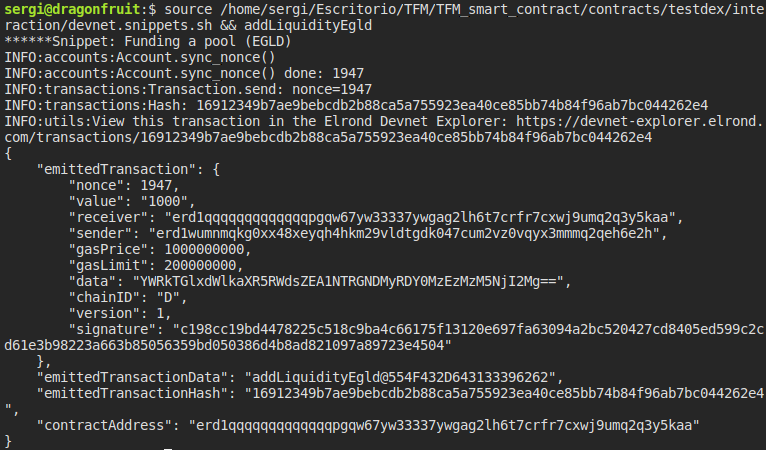
\includegraphics[width=\linewidth]{testsnipped-addegld.png}
	  \caption{``addLiquidityEgld''.}\label{fig:test-addegld}
	\end{subfigure}\hfill
	\begin{subfigure}[b]{0.47\textwidth}
	  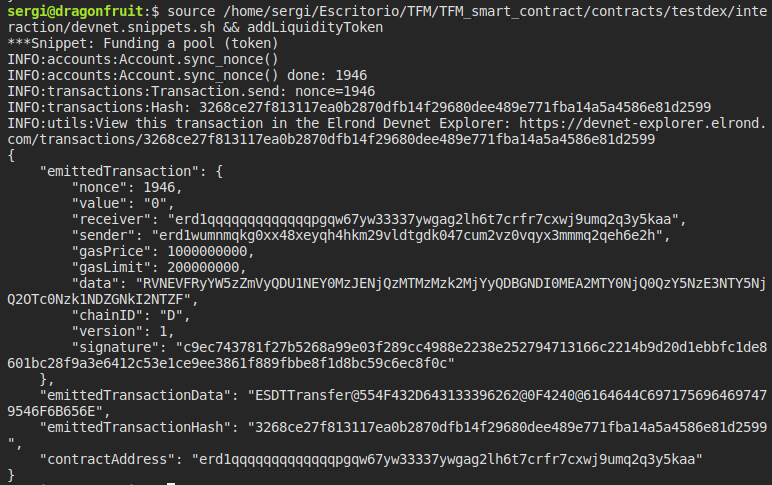
\includegraphics[width=\linewidth]{testsnipped-addtoken.png}
	  \caption{``addLiquidityToken''.}\label{fig:test-addtoken}
	\end{subfigure}\hfill
	\caption{Execució de proves per afegir un fons de liquiditat.}
\end{figure}

Finalment, Elrond disposa d'una eina anomenada \textbf{Mandos} i d'una \textbf{testnet} (local), que permeten \textbf{automatitzar les proves} en un entorn controlat (\cite{elrond2022}, seccions ``\textit{Mandos tests reference}'' i  ``\textit{Setup a Local Testnet}''). A part de per una qüestió merament de temps (són eines específiques que requereixen un temps d'aprenentatge i no podia abastar-ho tot), per l'objectiu de posar a prova el rediment de la xarxa Elrond he triat realitzar les proves directament a la devnet amb els \textit{snippets} (m'ha donat certa experiència de camp amb l'eina). 

\subsubsection{Sobre la DApp}
S'han comprovat manualment els casos d'ús descrits en la secció \ref{subsub:casosdus}:.
\begin{enumerate}
\item S'ha afegit liquiditat. En la finestra que apareix en l'opció ``Fund'' en la llista desplegable apareixen els \textit{tokens} disponibles al moneder de l'usuari que ha accedit a testDEX (Fig. \ref{fig:imp-liqpools2}). Al fons, quan estigui definit, no se li podrà afegir més quantitat d'actius. En qualsevol cas, si es tria el token que defineix el fons ha d'aparèixer la quantitat d'actius que té assignat (Fig. \ref{fig:imp-liqpools1}).
\item S'han realitzat \textit{swaps} confirmant que els resultats coincideixen amb l'anàlisi teòric fet a la secció \ref{subsub:dexamm}. En la Fig. \ref{fig:swaptests} es pot comprovar que coincideixen preus calculats, valors transferits i beneficis obtinguts.
\item S'han recuperat beneficis i fons. En la Fig. \ref{fig:imp-fons} es pot veure l'estat inicial del fons i com queda després de reclamar els beneficis i els fons en si mateixos.
\item En totes les finestres de la DApp es mostraran les transaccions relacionades. Filtro les transaccions segons els mètodes del contracte intel·ligent trucats. S'ha comprovat el correcte funcionament.
\end{enumerate}

Òbviament s'han emprat també els \textit{snippets} de l'apartat anterior per confirmar els resultats. M'hauria agradat automatitzar el procés de proves amb algun \textit{framework} de React però no he tingut temps material per formar-me.

\clearpage

\begin{figure}[!htb]
	\begin{subfigure}[b]{0.42\textwidth}
	  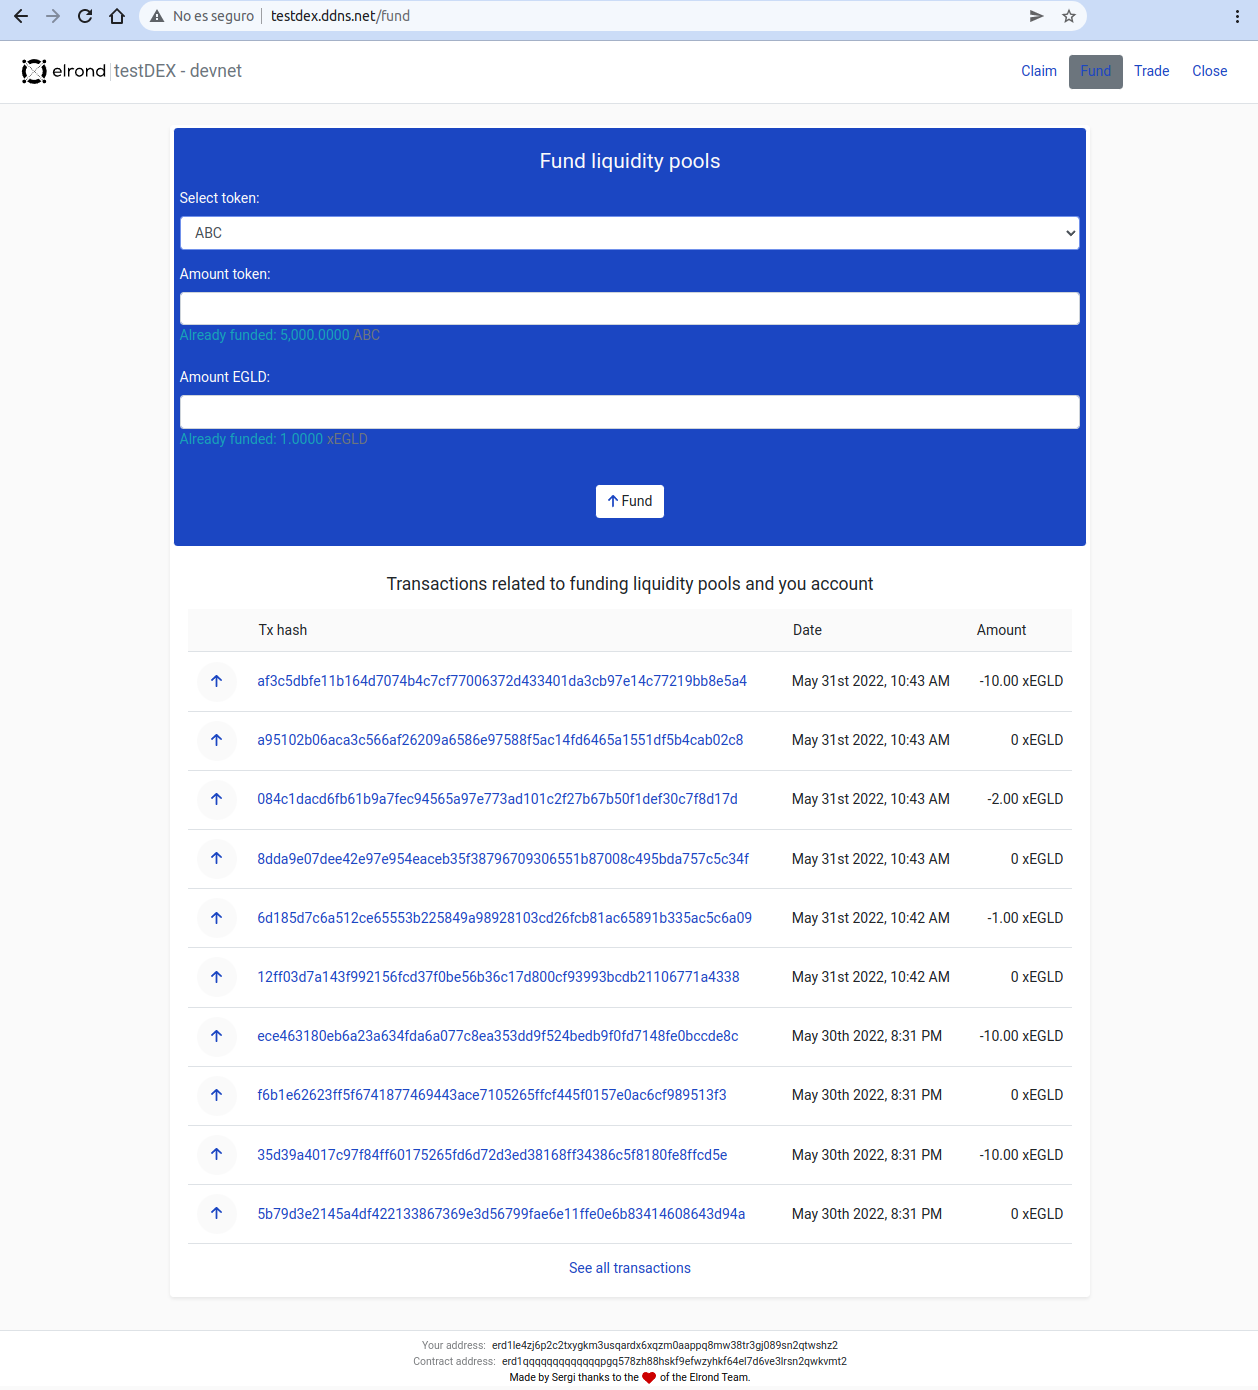
\includegraphics[width=\linewidth]{imp-liqpools1.png}
	  \caption{Estat del fons ABC-xEGLD.}\label{fig:imp-liqpools1}
	\end{subfigure}\hfill
	\begin{subfigure}[b]{0.42\textwidth}
	  \includegraphics[width=\linewidth]{imp-liqpools2.png}
	  \caption{\textit{Tokens} al \textit{wallet} del client.}\label{fig:imp-liqpools2}
	\end{subfigure}\hfill
	\caption{Fons de liquiditat creats.}
\end{figure}

\begin{figure}[!htb]
	\begin{subfigure}[b]{0.42\textwidth}
	  \includegraphics[width=\linewidth]{imp-price1.png}
	  \caption{Preu d'un xEGLD front a UOC.}\label{fig:imp-price1}
	\end{subfigure}\hfill
	\begin{subfigure}[b]{0.42\textwidth}
	  \includegraphics[width=\linewidth]{imp-price2.png}
	  \caption{\textit{Swap} d'un xEGLD per UOC.}\label{fig:imp-price2}
	\end{subfigure}\hfill
	\begin{subfigure}[b]{0.42\textwidth}
	  \includegraphics[width=\linewidth]{imp-price3.png}
	  \caption{Preu de mil xEGLD front a xEGLD.}\label{fig:imp-price3}
	\end{subfigure}\hfill
	\begin{subfigure}[b]{0.42\textwidth}
	  \includegraphics[width=\linewidth]{imp-price4.png}
	  \caption{Beneficis després de fer un \textit{swap} d'un xEGLD per UOC i seguit de 1000 UOC per xEGLD.}\label{fig:imp-price4}
	\end{subfigure}\hfill
	\caption{\textit{Swaps} realitzats segons allò descrit en la secció \ref{subsub:dexamm}.}
	\label{fig:swaptests}
\end{figure}

\begin{figure}[!htb]
	\begin{subfigure}[b]{0.3\textwidth}
	  \includegraphics[width=\linewidth]{imp-fons1.png}
	  \caption{Abans de reclamar.}\label{fig:imp-fons1}
	\end{subfigure}\hfill
	\begin{subfigure}[b]{0.3\textwidth}
	  \includegraphics[width=\linewidth]{imp-fons2.png}
	  \caption{Després de reclamar beneficis.}\label{fig:imp-fons2}
	\end{subfigure}\hfill
	\begin{subfigure}[b]{0.3\textwidth}
	  \includegraphics[width=\linewidth]{imp-fons3.png}
	  \caption{Després de reclamar el fons.}\label{fig:imp-fons3}
	\end{subfigure}\hfill
	\caption{Recuperació de fons de liquiditat i beneficis generats.}
	\label{fig:imp-fons}
\end{figure}

\subsubsection{Sobre el rendiment de la \textit{devnet} d'Elrond}
Un dels objectius del present treball és definir proves per comprovar les característiques de la xarxa Elrond. En la secció \ref{sub:xarxes} s'han comentat les característiques bàsiques de la \textit{devnet}, en la \ref{subsub:arq} l'arquitectura de testDEX i en la \ref{imp:aspectes} les diferents formes en què ens hem comunicat a la \textit{blockchain}. Tenint en compte tot això, amb la intenció de mesurar el temps que triga a realitzar les peticions s'ha realitzat un \textit{script} en Python, que com he dit es troba en el repositori TFM\_stats.

Les transaccions per unitat de temps poden ser un bon indicador per valorar el rendiment de la devnet. Com s'ha vist, si el moneder que envia la transacció es troba al mateix s\textit{hard} que el contracte intel·ligent la transacció serà més ràpida que si es troba en un altre \textit{shard}. Des de Python he trobat una solució per enviar transaccions en bloc, però per recuperar-les no he trobat forma de disparar automàticament una funció que tracti la resposta. Ho he implementat amb un bucle que demana les dades de les transaccions segons el seu \textit{hash} a l'API d'Elrond fins que totes tenen l'estat a ``\textit{success}''. Això s'ha de tenir en compte perquè els resultats que es mostren, per aquest motiu, tenen un retard afegit.

El que fa el \textit{script} és enviar un conjunt de transaccions que trucaran el mètode del contracte intel·ligent ``addLiquidityEgld'' passant-li com a paràmetre ``ABC-109739'' (un \textit{token} creat per mi). A més cada transacció transportarà un valor de 0,01 xEGLD. Amb això el que estem fent és fundar amb xEGLD el fons ABC-xEGLD. En la Fig. \ref{fig:send5trans} es veu un exemple d'execució per a un total de 5 transaccions\footnote{En el codi font han d'estar definits \({NUM\_TRANS=5}\) i \({PEM={'\texttildelow/wallet/wallet3.pem'}}\).} (5 transaccions executades en 2,896 segons).

Provant d'enviar un nombre més considerable de transaccions, m'he adonat que a partir de les 2500 transaccions el \textit{script} falla. Però per a 2000 ha obtingut que s'han realitzat en 7 minuts i 7 segons\footnote{En el codi font han d'estar definits \({NUM\_TRANS=2000}\) i \({PEM={'\texttildelow/wallet/wallet3.pem'}}\).}. S'ha de remarcar que això implica que s'han enviat 20 xEGLD al fons remartits entre 2000 transaccions (0.01 xEGLD/transacció). En la Fig. \ref{fig:send2000trans1} es pot veure una captura del resultat.	

Una altra prova obligada és fer les transaccions amb un moneder que es trobi en un altre \textit{shard}. Com que no serà el propietari del contracte intel·ligent, aquest respondrà que no pot fundar el fons. Això implica que la màquina virtual no executarà pràcticament codi. Per aquest motiu, he tornat a llançar el test amb un \textit{wallet} que no és propietari del contracte intel·ligent, però que es troba al mateix \textit{shard} (després ho provaré també amb un fragment diferent). En aquest darrer cas, per a 5 transaccions (Fig. \ref{fig:send5transnotowner}) ha trigat 1 segon (1852 ms) i per a 2000 ha tardat 7 minuts i 3 segons (Fig. \ref{fig:send2000transnotowner}).\footnote{En el codi font han d'estar definits \({NUM\_TRANS=5}\) o \({NUM\_TRANS=2000}\) i \({PEM={'\texttildelow/wallet/wallet1.pem'}}\).}

Dit tot això, la prova ja des d'un compte que no és propietari del contracte i que no es troba al mateix \textit{shard} ha trigat 31 segons per a 5 transaccions (Fig. \ref{fig:send5transnotownerothershards}) i per a 2000 transaccions 7 minuts i 31 segons (Fig. \ref{fig:send2000transnotownerothershards}).\footnote{En el codi font han d'estar definits \({NUM\_TRANS=5}\) o \({NUM\_TRANS=2000}\) i \({PEM={'\texttildelow/wallet/wallet2.pem'}}\).}

Totalitzant aquestes dades en una taula:

\begin{tabularx}{0.8\textwidth} { 
  | >{\raggedleft\arraybackslash}X 
  | >{\centering\arraybackslash}X
  | >{\centering\arraybackslash}X
  | >{\centering\arraybackslash}X 
  | >{\raggedleft\arraybackslash}X | }
 \hline
 \textbf{Núm. trans.} & \textit{\textbf{Shard}} & \textit{\textbf{Owner}} & \textbf{Figura} & \textbf{Temps (ms)} \\
 \hline
 5  & 0 & sí  & \ref{fig:send5trans} & 2151  \\
 \hline
 2000  & 0 & sí  & \ref{fig:send2000trans1} & 427788  \\
 \hline
 5  & 0 & no  & \ref{fig:send5transnotowner} & 1852  \\
 \hline
 2000  & 0 & no  & \ref{fig:send2000transnotowner} & 423468  \\
 \hline
 5  & 2 & no  & \ref{fig:send5transnotownerothershards} & 31094  \\
 \hline
 2000  & 2 & no  & \ref{fig:send2000transnotownerothershards} & 451136  \\
 \hline
\end{tabularx}

És molt petita la mostra per extreure conclusions fermes, però veiem que quan s'augmenta el nombre de transaccions enviades el temps que triga en els diferents casos convergeix. Amb 2000 transaccions el cas d'un remitent que no és propietari del \textit{smart contract} i que es troba en un altre \textit{shard} és només entorn d'un 5\% més lent. Tot això fa pensar que \textbf{l'arquitectura en \textit{shards} és eficient}. També s'ha de destacar, com s'ha dit en la secció \ref{sub:xarxes}, que la devnet té només 300 nodes validadors, enfront de la testnet i la mainnet que en tenen 3000. Per sortir de dubtes, he desplegat el contracte intel·ligent a la testnet amb:
\begin{lstlisting}[
    basicstyle=\footnotesize,
]
erdpy contract deploy --pem="~/wallet/wallet3.pem" \
  --recall-nonce --gas-limit=100000000 --project=. \
  --proxy="https://testnet-gateway.elrond.com" \
  --chain="T" --arguments 0x05 --send
\end{lstlisting}

I he tornat a fer la prova amb 2000 transaccions\footnote{En el codi font han d'estar ha d'estar definit \({NUM\_TRANS=2000}\), \({PEM={'\texttildelow/wallet/wallet3.pem'}}\), \({CHAIN\_ID={'T'}}\) i \(CONTRACT\_ADDRESS={'erd1qqqqqqqqqqqqqpgqs3mnl4qnqrenzmaezf72vzeg5snpe9p0sn2qveucs5'}\).}. Sorprenetment, s'han executat en 8 minuts i 56 segons (536538 ms). Es pot veure una captura en la Fig. \ref{fig:sendtesnet}.
\begin{figure}[h]
\includegraphics[width=0.99\textwidth]{send5trans.png}
\centering
\caption{Resultat del \textit{script} de Python executat per a 5 transaccions.}\label{fig:send5trans}
\end{figure} 

\begin{figure}[h]
\includegraphics[width=0.99\textwidth]{send2000trans1.png}
\centering
\caption{Resultat del \textit{script} de Python executat per a 2000 transaccions (es mostren només els darrer \textit{hashes}).}\label{fig:send2000trans1}
\end{figure} 

\begin{figure}[h]
\includegraphics[width=0.99\textwidth]{send5transnotowner.png}
\centering
\caption{Resultat del \textit{script} de Python executat per a 5 transaccions amb un remitent que no és el propietari del \textit{smart contract} però que es troba al mateix \textit{shard}.}\label{fig:send5transnotowner}
\end{figure} 

\begin{figure}[h]
\includegraphics[width=0.99\textwidth]{send2000transnotowner.png}
\centering
\caption{Resultat del \textit{script} de Python executat per a 2000 transaccions amb un remitent que no és el propietari del \textit{smart contract} però que es troba al mateix \textit{shard}.}\label{fig:send2000transnotowner}
\end{figure} 

\begin{figure}[h]
\includegraphics[width=0.99\textwidth]{send5transnotownerothershards.png}
\centering
\caption{Resultat del \textit{script} de Python executat per a 5 transaccions amb un remitent que no és el propietari del \textit{smart contract} i que a més no es troba al mateix \textit{shard}.}\label{fig:send5transnotownerothershards}
\end{figure} 

\begin{figure}[h]
\includegraphics[width=0.99\textwidth]{send2000transnotownerothershards.png}
\centering
\caption{Resultat del \textit{script} de Python executat per a 2000 transaccions amb un remitent que no és el propietari del \textit{smart contract} i que a més no es troba al mateix \textit{shard}.}\label{fig:send2000transnotownerothershards}
\end{figure} 

\begin{figure}[h]
\includegraphics[width=0.99\textwidth]{sendtestnet.png}
\centering
\caption{Resultat del \textit{script} de Python executat per a 2000 transaccions em a testnet.}\label{fig:sendtesnet}
\end{figure} 

\clearpage

\section{Conclusions}\label{sec:con}
Déu-n'hi-do per arribar fins aquí. Era allunyat de la programació de fa més de deu anys i ha estat un camí pedregós. Tampoc tenia gaire idea de \textit{blockchain} (no he cursat l'assignatura). En qualsevol cas, que hagi pogut finalitzar el present treball és bona mostra de què \textbf{l'entorn d'Elrond és força amigable per al programador} (punt important per a la seva adopció). Aquesta companyia ha avançat molt ràpidament i, tot i que han desenvolupat molts de continguts per a aprendre la seva tecnologia, podrien estar millor (sobretot penso que falten exemples amb codi font executable del que s'explica a \cite{elrond2022}). Com que és un projecte relativament recent, no trobes gaire codi a Github, no hi ha cap curs a Udemy o altres plataformes (Ethereum té una gran comunitat de desenvolupadors i molt de material disponible). Per contra, simplement provant testDEX, veus que \textbf{les transaccions van força més ràpid que amb Ethereum}. Diferents fonts --com \cite{mincub2019-2} o \cite{everstake2020}-- parlem de més de 10000 TPS. Imagino que els meus resultats són més discrets en fer proves en una xarxa configurada amb només 3 \textit{shards}\footnote{``\textit{Testnet exceeded 12k TPS with only 5 shards and 65k with 20 shards} [...]'' (\cite{paradigm2019}). }, per la penalització en temps induïda per la meva implementació i per les eines emprades (que possiblement són limitades).

Penso que el present treball revisa la tecnologia d'Elrond amb un mínim de rigor acadèmic, que s'ha realitzat un exemple pràctic (molt millorable per la meva inexperiència com a programador) i que s'ha comprovat el funcionament de la xarxa Elrond d'una forma molt bàsica. Per altra banda, aquest treball possiblement sigui un dels primers en llengua catalana emprant aquesta tecnologia. En la secció \ref{sub:objectius} no he citat el meu objectiu personal, que era bàsicament aprendre. Penso que això sí que s'ha assolit al 150\%.

Com a \textbf{crítica personal}, la meva falta de coneixements i d'experiència en el desenvolupament de programari ha fet que em desviï uns quants dies en la planificació prevista. Inicialment, en el disseny vaig plasmar que volia fer també un gràfic sobre l'evolució dels preus, però vaig haver de retallar el projecte un poc per falta de temps (he de dir que he hagut de dedicar-ne més del que esperava). També el \textit{script} en Python es podria haver parametritzat i haver fet més genèric (sé que són unes poques hores de feina). O ha faltat emprar alguna bona metodologia per fer proves mentre s'implementava la DApp. En definitiva, em quedo amb un regust agredolç.

Com a \textbf{línies de treball futures}, parlant a títol personal, ara tinc clara una línia de formació que he de seguir per suplir les meves carències. El meu perfil és més de sistemes i de sistemes gestors de bases de dades, però m'està fascinant el món de les cadenes de blocs. Vull formar-me en React i Rust i refer tot el codi (o tal vegada fer-ne un de nou relacionat amb NFT). Pel que fa a potencials futurs treballs de final de grau o de màster, la part d'estudi del rendiment en TPS és un bon filó per explotar (tot i que penso que sense la col·laboració de l'equip d'Elrond en algunes coses pot ser complicat). Tampoc no s'ha fet cap estudi de les despeses que duen associades les transaccions (punt on Elrond és també superior a Ethereum \cite{paradigm2019,everstake2020}). Per altra banda, penso que la meva idea original de fer un bon material didàctic amb exemples per aprendre a desenvolupar en la tecnologia Elrond seria força interessant (per la falta de material en general). Finalment, els problemes exposats per a la constant \(k\) donen per a una bona revisió bibliogràfica sobre el tema (com \cite{zhang2018}).

La meva \textbf{conclusió final}, dins de la meva humil opinió de neòfit en el món del \textit{blockchain}, és que tenint en compte l'eficiència de la xarxa, la limitació en el cost de les transaccions i el maquinari genèric que es necessita per poder posar en producció un node de la xarxa\footnote{Aquest punt pot ser controvertit per la quantitat d'EGLD que s'ha de mantenir en \textit{staking} (en l'hipotètic escenari que pugi molt de preu).}, la tecnologia d'\textbf{Elrond és encara infravalorada}.

\newpage 


\section{Glossari}\label{sec:glo}
\begin{itemize}
\item \textbf{AMM (\textit{Automated Market Makers})}: Protocol que determina automàticament els preus d'un parell d'actius que conformen un fons de liquiditat.
\item \textbf{\textit{Blockchain} (cadena de blocs)}: Base de dades distribuïda de comptabilitat que es comparteix entre els nodes d'una xarxa informàtica sense una autoritat central que els gestioni.
\item \textbf{DApp (\textit{Decentralized Application})}: És una aplicació que funciona sense la necessitat de servidors centrals (gràcies a la tecnologia \textit{blockchain}).
\item \textbf{DEX (\textit{Decentralized EXchange})}: Mercat d'igual a igual on les transaccions es produeixen directament entre els usuaris sense la intervenció de cap autoritat de control central.
\item \textbf{PoW (\textit{Proof of Work})}: És un protocol de consens en sistemes descentralitzats que per verificar els blocs i les transaccions requereix els membres de la xarxa que resolguin un problema matemàtic arbitrari que duu associat un càlcul considerable, evitant així que ningú utilitzi de forma il·lícita el sistema.
\item \textbf{PoS (\textit{Proof of Stake})}: Alternativa a PoW que redueix la potència de càlcul associada per verificar els blocs i les transaccions gràcies a un algoritme de consens amb la participació de nodes validadors que han d'aportar criptoactius com a fiança (\textit{stake}).
\item \textbf{\textit{Smart contract}}: Contracte emmagatzemat en una \textit{blockchain} que permet l'execució automàtica de certs termes acordats gràcies a un programa informàtic.
\item \textbf{\textit{Token}}: Unitat de valor fonamentada en la criptografia i \textit{blockchain}.
\end{itemize}

\newpage 


\section{Bibliografia}\label{sec:bib}
\bibliographystyle{IEEEtran}
\bibliography{IEEEabrv,sources}

\newpage 


\section{Annexos}\label{sec:ann}
\subsection{Breu manual d'usuari de testDEX}\label{sub:manual}
\subsubsection{Introducció}
L'aplicació bàsicament té dos perfils d'usuari:
\begin{itemize}
\item Propietari del contracte intel·ligent: Podrà accedir a totes les opcions del menú.
\item Resta d'usuaris de la xarxa Elrond: Podran accedir només a l'opció ``Trading''.
\end{itemize}

\subsubsection{Opció ``Fund''}
Permet el propietari del contracte intel·ligent fundar un \textit{liquidity pool}. En la llista desplegable ``Select token'' li apareixeran els diferents tokens ESDT disponibles en la seva cartera. Es triarà un d'aquests tokens (``Select token'') i se li afegirà una quantitat determinada del mateix (``Amount token'') i una altra quantitat de xEGLD (``Amount EGLD''). Una vegada fundat el fons no se li podem afegir més actius (a no ser que es reclami i es torni a fundar). Quan se seleccioni un token es mostraran la quantitat d'actius pels quals està format (camps ``Already funded'').
\begin{figure}[h]
\includegraphics[width=0.6\textwidth]{manualfund.png}
\centering
\caption{Opció ``Fund'' a testDEX.}\label{fig:manualfund}
\end{figure} 

\subsubsection{Opció ``Claim''}
Permet el propietari del contracte intel·ligent recuperar els fons de liquiditat o bé els seus beneficis. Basta triar un \textit{token} de la llista desplegable (``Select pair'') i prémer el botó ``Claim earnings'' o bé ``Claim pool'' (es mostraran només els \textit{pools} disponibles en el \textit{smart contract}). S'ha de destacar que quan es recuperin els beneficis d'un \textit{pool} es recuperarà el xEGLD de tots (no només del parell definit pel \textbf{token} seleccionat). Quan se seleccioni un token es mostraran la quantitat d'actius pels quals està format el fons i els beneficis disponibles (camps ``Pool available'' i camp ``Earnings available'').

\begin{figure}[h]
\includegraphics[width=0.6\textwidth]{manualclaim.png}
\centering
\caption{Opció ``Claim'' a testDEX.}\label{fig:manualclaim}
\end{figure} 

\subsubsection{Opció ``Trade''}
En la llista desplegable es podran seleccionar els parells disponibles en el contracte intel·ligent per fer \textit{trading}. Quan es triï un parell es mostraran les quantitats dels actius disponibles en el \textit{pool} i en el moneder de l'usuari (camps ``Pool (amount available)'' i ``Your wallet (amount available)''). En introduir una quantitat (``Amount''), es calcularà automàticament tant el preu de compra com el de venda (camps ``Buy'' i ``Sell'').

Un darrer comentari és que no s'ha limitat l'entrada de nombres que l'usuari pot introduir al quadre de text amb la quantitat. Així es pot provar el comportament del contracte intel·ligent en casos extrems.
\begin{figure}[h]
\includegraphics[width=0.6\textwidth]{manualtrade.png}
\centering
\caption{Opció ``Claim'' a testDEX.}\label{fig:manualtrade}
\end{figure} 

\end{document}
